\documentclass[twoside]{book}

% Packages required by doxygen
\usepackage{calc}
\usepackage{doxygen}
\usepackage{graphicx}
\usepackage[utf8]{inputenc}
\usepackage{makeidx}
\usepackage{multicol}
\usepackage{multirow}
\usepackage{textcomp}
\usepackage[table]{xcolor}

% Font selection
\usepackage[T1]{fontenc}
\usepackage{mathptmx}
\usepackage[scaled=.90]{helvet}
\usepackage{courier}
\usepackage{amssymb}
\usepackage{sectsty}
\renewcommand{\familydefault}{\sfdefault}
\allsectionsfont{%
  \fontseries{bc}\selectfont%
  \color{darkgray}%
}
\renewcommand{\DoxyLabelFont}{%
  \fontseries{bc}\selectfont%
  \color{darkgray}%
}

% Page & text layout
\usepackage{geometry}
\geometry{%
  a4paper,%
  top=2.5cm,%
  bottom=2.5cm,%
  left=2.5cm,%
  right=2.5cm%
}
\tolerance=750
\hfuzz=15pt
\hbadness=750
\setlength{\emergencystretch}{15pt}
\setlength{\parindent}{0cm}
\setlength{\parskip}{0.2cm}
\makeatletter
\renewcommand{\paragraph}{%
  \@startsection{paragraph}{4}{0ex}{-1.0ex}{1.0ex}{%
    \normalfont\normalsize\bfseries\SS@parafont%
  }%
}
\renewcommand{\subparagraph}{%
  \@startsection{subparagraph}{5}{0ex}{-1.0ex}{1.0ex}{%
    \normalfont\normalsize\bfseries\SS@subparafont%
  }%
}
\makeatother

% Headers & footers
\usepackage{fancyhdr}
\pagestyle{fancyplain}
\fancyhead[LE]{\fancyplain{}{\bfseries\thepage}}
\fancyhead[CE]{\fancyplain{}{}}
\fancyhead[RE]{\fancyplain{}{\bfseries\leftmark}}
\fancyhead[LO]{\fancyplain{}{\bfseries\rightmark}}
\fancyhead[CO]{\fancyplain{}{}}
\fancyhead[RO]{\fancyplain{}{\bfseries\thepage}}
\fancyfoot[LE]{\fancyplain{}{}}
\fancyfoot[CE]{\fancyplain{}{}}
\fancyfoot[RE]{\fancyplain{}{\bfseries\scriptsize Generated on Wed Sep 14 2016 15\-:28\-:45 for Hi\-Q\-P\-\_\-\-Controllers R\-O\-S Package by Doxygen }}
\fancyfoot[LO]{\fancyplain{}{\bfseries\scriptsize Generated on Wed Sep 14 2016 15\-:28\-:45 for Hi\-Q\-P\-\_\-\-Controllers R\-O\-S Package by Doxygen }}
\fancyfoot[CO]{\fancyplain{}{}}
\fancyfoot[RO]{\fancyplain{}{}}
\renewcommand{\footrulewidth}{0.4pt}
\renewcommand{\chaptermark}[1]{%
  \markboth{#1}{}%
}
\renewcommand{\sectionmark}[1]{%
  \markright{\thesection\ #1}%
}

% Indices & bibliography
\usepackage{natbib}
\usepackage[titles]{tocloft}
\setcounter{tocdepth}{3}
\setcounter{secnumdepth}{5}
\makeindex

% Hyperlinks (required, but should be loaded last)
\usepackage{ifpdf}
\ifpdf
  \usepackage[pdftex,pagebackref=true]{hyperref}
\else
  \usepackage[ps2pdf,pagebackref=true]{hyperref}
\fi
\hypersetup{%
  colorlinks=true,%
  linkcolor=blue,%
  citecolor=blue,%
  unicode%
}

% Custom commands
\newcommand{\clearemptydoublepage}{%
  \newpage{\pagestyle{empty}\cleardoublepage}%
}


%===== C O N T E N T S =====

\begin{document}

% Titlepage & ToC
\hypersetup{pageanchor=false}
\pagenumbering{roman}
\begin{titlepage}
\vspace*{7cm}
\begin{center}%
{\Large Hi\-Q\-P\-\_\-\-Controllers R\-O\-S Package }\\
\vspace*{1cm}
{\large Generated by Doxygen 1.8.6}\\
\vspace*{0.5cm}
{\small Wed Sep 14 2016 15:28:45}\\
\end{center}
\end{titlepage}
\clearemptydoublepage
\tableofcontents
\clearemptydoublepage
\pagenumbering{arabic}
\hypersetup{pageanchor=true}

%--- Begin generated contents ---
\chapter{Todo List}
\label{todo}
\hypertarget{todo}{}

\begin{DoxyRefList}
\item[\label{todo__todo000002}%
\hypertarget{todo__todo000002}{}%
Member \hyperlink{classhiqp_1_1geometric__primitives_1_1GeometricPrimitiveMap_aed92b78b51ccd075d226b003f9576476}{hiqp\-:\-:geometric\-\_\-primitives\-:\-:Geometric\-Primitive\-Map\-:\-:clear} ()]primitives with dependencies to tasks shall not be deleted!  
\item[\label{todo__todo000001}%
\hypertarget{todo__todo000001}{}%
Member \hyperlink{classhiqp_1_1geometric__primitives_1_1GeometricPrimitiveMap_a07d04c1a3bb164bb501bd03cc6bc1eae}{hiqp\-:\-:geometric\-\_\-primitives\-:\-:Geometric\-Primitive\-Map\-:\-:remove\-Geometric\-Primitive} (std\-::string name)]primitives should have dependencies on tasks and not be removable if dependencies exists!  
\item[\label{todo__todo000004}%
\hypertarget{todo__todo000004}{}%
Member \hyperlink{classhiqp_1_1TaskManager_a1f58d497fa59e23506e6d7d60fe3693d}{hiqp\-:\-:Task\-Manager\-:\-:remove\-Task} (std\-::string task\-\_\-name)]removal of tasks must also delete task dynamics or else there's a memory leak!  
\item[\label{todo__todo000003}%
\hypertarget{todo__todo000003}{}%
Member \hyperlink{classhiqp_1_1TaskManager_a688ad548e2ef681b458c1fc90326f6e6}{hiqp\-:\-:Task\-Manager\-:\-:$\sim$\-Task\-Manager} () noexcept]cleanup of tasks and task dynamics is missing! 
\end{DoxyRefList}
\chapter{Namespace Index}
\section{Namespace List}
Here is a list of all documented namespaces with brief descriptions\-:\begin{DoxyCompactList}
\item\contentsline{section}{\hyperlink{namespacehiqp}{hiqp} }{\pageref{namespacehiqp}}{}
\end{DoxyCompactList}

\chapter{Hierarchical Index}
\section{Class Hierarchy}
This inheritance list is sorted roughly, but not completely, alphabetically\-:\begin{DoxyCompactList}
\item Joint\-Velocity\-Controller\begin{DoxyCompactList}
\item \contentsline{section}{hiqp\-:\-:Hi\-Q\-P\-\_\-\-Kinematic\-\_\-\-Controller}{\pageref{classhiqp_1_1HiQP__Kinematic__Controller}}{}
\end{DoxyCompactList}
\item \contentsline{section}{hiqp\-:\-:Task}{\pageref{classhiqp_1_1Task}}{}
\item \contentsline{section}{hiqp\-:\-:Task\-Manager}{\pageref{classhiqp_1_1TaskManager}}{}
\end{DoxyCompactList}

\chapter{Class Index}
\section{Class List}
Here are the classes, structs, unions and interfaces with brief descriptions\-:\begin{DoxyCompactList}
\item\contentsline{section}{\hyperlink{classhiqp_1_1HiQP__Kinematic__Controller}{hiqp\-::\-Hi\-Q\-P\-\_\-\-Kinematic\-\_\-\-Controller} \\*This is my awesome controller }{\pageref{classhiqp_1_1HiQP__Kinematic__Controller}}{}
\end{DoxyCompactList}

\chapter{File Index}
\section{File List}
Here is a list of all documented files with brief descriptions\-:\begin{DoxyCompactList}
\item\contentsline{section}{include/hiqp/\hyperlink{hiqp__kinematic__controller_8h}{hiqp\-\_\-kinematic\-\_\-controller.\-h} \\*Brief description of file }{\pageref{hiqp__kinematic__controller_8h}}{}
\item\contentsline{section}{include/hiqp/\hyperlink{hiqp__utils_8h}{hiqp\-\_\-utils.\-h} \\*Brief description of file }{\pageref{hiqp__utils_8h}}{}
\item\contentsline{section}{include/hiqp/\hyperlink{task_8h}{task.\-h} \\*Brief description of file }{\pageref{task_8h}}{}
\item\contentsline{section}{include/hiqp/\hyperlink{task__beh__fo_8h}{task\-\_\-beh\-\_\-fo.\-h} \\*Brief description of file }{\pageref{task__beh__fo_8h}}{}
\item\contentsline{section}{include/hiqp/\hyperlink{task__behaviour_8h}{task\-\_\-behaviour.\-h} \\*Brief description of file }{\pageref{task__behaviour_8h}}{}
\item\contentsline{section}{include/hiqp/\hyperlink{task__manager_8h}{task\-\_\-manager.\-h} \\*Brief description of file }{\pageref{task__manager_8h}}{}
\item\contentsline{section}{include/hiqp/\hyperlink{task__pop_8h}{task\-\_\-pop.\-h} \\*Brief description of file }{\pageref{task__pop_8h}}{}
\item\contentsline{section}{include/hiqp/\hyperlink{task__visualizer_8h}{task\-\_\-visualizer.\-h} \\*Brief description of file }{\pageref{task__visualizer_8h}}{}
\item\contentsline{section}{src/\hyperlink{hiqp__kinematic__controller_8cpp}{hiqp\-\_\-kinematic\-\_\-controller.\-cpp} \\*Brief description of file }{\pageref{hiqp__kinematic__controller_8cpp}}{}
\item\contentsline{section}{src/\hyperlink{hiqp__utils_8cpp}{hiqp\-\_\-utils.\-cpp} \\*Brief description of file }{\pageref{hiqp__utils_8cpp}}{}
\item\contentsline{section}{src/\hyperlink{task__beh__fo_8cpp}{task\-\_\-beh\-\_\-fo.\-cpp} \\*Brief description of file }{\pageref{task__beh__fo_8cpp}}{}
\item\contentsline{section}{src/\hyperlink{task__manager_8cpp}{task\-\_\-manager.\-cpp} \\*Brief description of file }{\pageref{task__manager_8cpp}}{}
\item\contentsline{section}{src/\hyperlink{task__pop_8cpp}{task\-\_\-pop.\-cpp} \\*Brief description of file }{\pageref{task__pop_8cpp}}{}
\item\contentsline{section}{src/\hyperlink{task__visualizer_8cpp}{task\-\_\-visualizer.\-cpp} \\*Brief description of file }{\pageref{task__visualizer_8cpp}}{}
\end{DoxyCompactList}

\chapter{Namespace Documentation}
\hypertarget{namespacehiqp}{\section{hiqp Namespace Reference}
\label{namespacehiqp}\index{hiqp@{hiqp}}
}
\subsection*{Classes}
\begin{DoxyCompactItemize}
\item 
struct \hyperlink{structhiqp_1_1HiQPStage}{Hi\-Q\-P\-Stage}
\item 
class \hyperlink{classhiqp_1_1HiQPSolver}{Hi\-Q\-P\-Solver}
\item 
class \hyperlink{classhiqp_1_1HiQPTimePoint}{Hi\-Q\-P\-Time\-Point}
\begin{DoxyCompactList}\small\item\em The time type used in this framework. \end{DoxyCompactList}\item 
class \hyperlink{classhiqp_1_1ROSDynamicsController}{R\-O\-S\-Dynamics\-Controller}
\begin{DoxyCompactList}\small\item\em This is my awesome controller. \end{DoxyCompactList}\item 
class \hyperlink{classhiqp_1_1ROSKinematicsController}{R\-O\-S\-Kinematics\-Controller}
\item 
class \hyperlink{classhiqp_1_1ROSTopicSubscriber}{R\-O\-S\-Topic\-Subscriber}
\item 
class \hyperlink{classhiqp_1_1ROSVisualizer}{R\-O\-S\-Visualizer}
\item 
class \hyperlink{classhiqp_1_1CasADiSolver}{Cas\-A\-Di\-Solver}
\item 
class \hyperlink{classhiqp_1_1TaskDynamics}{Task\-Dynamics}
\item 
class \hyperlink{classhiqp_1_1TaskFactory}{Task\-Factory}
\begin{DoxyCompactList}\small\item\em A factory for creating task function and task dynamics. (The process of creating and initializing them is intertwined.) \end{DoxyCompactList}\item 
class \hyperlink{classhiqp_1_1TaskFunction}{Task\-Function}
\item 
class \hyperlink{classhiqp_1_1TaskMonitoringData}{Task\-Monitoring\-Data}
\begin{DoxyCompactList}\small\item\em An aggregation of const references to facilitate communication of monitoring data. \end{DoxyCompactList}\item 
class \hyperlink{classhiqp_1_1TaskManager}{Task\-Manager}
\begin{DoxyCompactList}\small\item\em Should be created only once! \end{DoxyCompactList}\item 
class \hyperlink{classhiqp_1_1DynamicsFirstOrder}{Dynamics\-First\-Order}
\begin{DoxyCompactList}\small\item\em A general first-\/order task dynamics implementation that enforces an exponential decay of the task function value. \end{DoxyCompactList}\item 
class \hyperlink{classhiqp_1_1DynamicsJntLimits}{Dynamics\-Jnt\-Limits}
\item 
class \hyperlink{classhiqp_1_1DynamicsMinimalJerk}{Dynamics\-Minimal\-Jerk}
\item 
class \hyperlink{classhiqp_1_1TaskFullPose}{Task\-Full\-Pose}
\begin{DoxyCompactList}\small\item\em Represents a task that sets a specific joint configuration. \end{DoxyCompactList}\item 
class \hyperlink{classhiqp_1_1TaskGeometricAlignment}{Task\-Geometric\-Alignment}
\item 
class \hyperlink{classhiqp_1_1TaskGeometricProjection}{Task\-Geometric\-Projection}
\begin{DoxyCompactList}\small\item\em It's awesome! \end{DoxyCompactList}\item 
class \hyperlink{classhiqp_1_1TaskJntConfig}{Task\-Jnt\-Config}
\begin{DoxyCompactList}\small\item\em Represents a task that sets a specific joint configuration. \end{DoxyCompactList}\item 
class \hyperlink{classhiqp_1_1TaskJntLimits}{Task\-Jnt\-Limits}
\item 
class \hyperlink{classhiqp_1_1Visualizer}{Visualizer}
\end{DoxyCompactItemize}
\subsection*{Typedefs}
\begin{DoxyCompactItemize}
\item 
typedef \\*
controller\-\_\-interface\-::\-Controller\\*
$<$ hardware\-\_\-interface\-::\-Velocity\-Joint\-Interface $>$ \hyperlink{namespacehiqp_a7b250295f6797153486ce8ab085bd450}{Joint\-Velocity\-Controller}
\item 
typedef \\*
hardware\-\_\-interface\-::\-Velocity\-Joint\-Interface \hyperlink{namespacehiqp_ac536ca3b4ba33489281fa5bec490799c}{Joint\-Velocity\-Interface}
\end{DoxyCompactItemize}
\subsection*{Functions}
\begin{DoxyCompactItemize}
\item 
\hypertarget{namespacehiqp_ae25bb9b7205ab2630606197e8a35af8f}{std\-::ostream \& {\bfseries operator$<$$<$} (std\-::ostream \&os, const K\-D\-L\-::\-Vector \&kdl\-\_\-vector)}\label{namespacehiqp_ae25bb9b7205ab2630606197e8a35af8f}

\item 
\hypertarget{namespacehiqp_ace17cd6f24f52ba09f129ab50f435f99}{std\-::ostream \& {\bfseries operator$<$$<$} (std\-::ostream \&os, const K\-D\-L\-::\-Tree \&kdl\-\_\-tree)}\label{namespacehiqp_ace17cd6f24f52ba09f129ab50f435f99}

\item 
\hypertarget{namespacehiqp_a59fe109d0df644e9ead2b56f8d86bf89}{std\-::ostream \& {\bfseries operator$<$$<$} (std\-::ostream \&os, const K\-D\-L\-::\-Frame\-Vel \&kdl\-\_\-frame\-\_\-vel)}\label{namespacehiqp_a59fe109d0df644e9ead2b56f8d86bf89}

\item 
\hypertarget{namespacehiqp_a33d4a297971bc3e2996aa1f3194b0e30}{std\-::ostream \& {\bfseries operator$<$$<$} (std\-::ostream \&os, const K\-D\-L\-::\-Jnt\-Array\-Vel \&kdl\-\_\-joints\-\_\-vel)}\label{namespacehiqp_a33d4a297971bc3e2996aa1f3194b0e30}

\item 
\hypertarget{namespacehiqp_a6a26da69453463527d0b4c99884983c9}{std\-::ostream \& {\bfseries operator$<$$<$} (std\-::ostream \&os, const K\-D\-L\-::\-Chain \&kdl\-\_\-chain)}\label{namespacehiqp_a6a26da69453463527d0b4c99884983c9}

\item 
\hypertarget{namespacehiqp_a95f3af7af45e7c81eda13572f2d3cc38}{int {\bfseries kdl\-\_\-get\-Q\-Nr\-From\-Joint\-Name} (const K\-D\-L\-::\-Tree \&kdl\-\_\-tree, const std\-::string \&joint\-\_\-name)}\label{namespacehiqp_a95f3af7af45e7c81eda13572f2d3cc38}

\item 
\hypertarget{namespacehiqp_afc65617e444dcefe5ca39e0dac2a17b2}{int {\bfseries kdl\-\_\-get\-Q\-Nr\-From\-Link\-Name} (const K\-D\-L\-::\-Tree \&kdl\-\_\-tree, const std\-::string \&link\-\_\-name)}\label{namespacehiqp_afc65617e444dcefe5ca39e0dac2a17b2}

\item 
\hypertarget{namespacehiqp_a9266d35577397a64d24935da167b406a}{int {\bfseries kdl\-\_\-\-Jnt\-To\-Jac} (const K\-D\-L\-::\-Tree \&tree, const K\-D\-L\-::\-Jnt\-Array\-Vel \&qqdot, K\-D\-L\-::\-Jacobian \&jac, const std\-::string \&segmentname)}\label{namespacehiqp_a9266d35577397a64d24935da167b406a}

\item 
\hypertarget{namespacehiqp_aed9588cb786450e506ca68402880b1d8}{void {\bfseries print\-Hiqp\-Info} (const std\-::string \&msg)}\label{namespacehiqp_aed9588cb786450e506ca68402880b1d8}

\item 
\hypertarget{namespacehiqp_a0993b019bfc0f0e2b38e76b2979eb0e0}{void {\bfseries print\-Hiqp\-Warning} (const std\-::string \&msg)}\label{namespacehiqp_a0993b019bfc0f0e2b38e76b2979eb0e0}

\item 
{\footnotesize template$<$typename Derived $>$ }\\Derived \hyperlink{namespacehiqp_a5762e31938369b2fdbd81ac2bd11ca0f}{pinv} (const Eigen\-::\-Matrix\-Base$<$ Derived $>$ \&a)
\begin{DoxyCompactList}\small\item\em calculates the Moore-\/\-Penrose Pseudoinverse for any sized matrices. \end{DoxyCompactList}\item 
{\footnotesize template$<$typename Derived $>$ }\\Derived \hyperlink{namespacehiqp_a8fb181f069898cddd461b0a33f2f19d1}{dls} (const Eigen\-::\-Matrix\-Base$<$ Derived $>$ \&a, double eta=0.\-01)
\begin{DoxyCompactList}\small\item\em calculates the Damped-\/\-Least-\/\-Square matrix. \end{DoxyCompactList}\item 
\hypertarget{namespacehiqp_a8c04766c4d507563fca71bb11f6beefe}{void {\bfseries print\-Children\-To\-Ostream} (std\-::ostream \&os, const std\-::vector$<$ K\-D\-L\-::\-Segment\-Map\-::const\-\_\-iterator $>$ \&children, std\-::vector$<$ bool $>$ \&is\-\_\-last\-\_\-child, unsigned int level=0)}\label{namespacehiqp_a8c04766c4d507563fca71bb11f6beefe}

\item 
\hypertarget{namespacehiqp_ad0fa6310317e1eef2829957a9b6c0b25}{{\footnotesize template$<$$>$ }\\void {\bfseries R\-O\-S\-Topic\-Subscriber\-::topic\-Callback$<$ geometry\-\_\-msgs\-::\-Pose\-Stamped $>$} (const geometry\-\_\-msgs\-::\-Pose\-Stamped \&msg)}\label{namespacehiqp_ad0fa6310317e1eef2829957a9b6c0b25}

\item 
\hypertarget{namespacehiqp_af211bffb33b796b259656fa391364046}{{\footnotesize template$<$$>$ }\\void {\bfseries R\-O\-S\-Topic\-Subscriber\-::topic\-Callback$<$ hiqp\-\_\-msgs\-\_\-srvs\-::\-Vector3d $>$} (const hiqp\-\_\-msgs\-\_\-srvs\-::\-Vector3d \&msg)}\label{namespacehiqp_af211bffb33b796b259656fa391364046}

\item 
\hypertarget{namespacehiqp_ac9939acdaf35ca4f7c41ea2d0b4f56c1}{std\-::string {\bfseries dtostr} (double d)}\label{namespacehiqp_ac9939acdaf35ca4f7c41ea2d0b4f56c1}

\item 
\hypertarget{namespacehiqp_a24b6e4f1d69ef88dd04cf5479693fca4}{std\-::ostream \& {\bfseries operator$<$$<$} (std\-::ostream \&os, const \hyperlink{structhiqp_1_1HiQPStage}{Hi\-Q\-P\-Stage} \&stage)}\label{namespacehiqp_a24b6e4f1d69ef88dd04cf5479693fca4}

\end{DoxyCompactItemize}
\subsection*{Variables}
\begin{DoxyCompactItemize}
\item 
\hypertarget{namespacehiqp_a0f68bffaa9135d62b92656c4c9e06a0b}{const double {\bfseries k\-Damping\-Factor} = 1e-\/5}\label{namespacehiqp_a0f68bffaa9135d62b92656c4c9e06a0b}

\end{DoxyCompactItemize}


\subsection{Detailed Description}
namespace for Hi\-Q\-P-\/related stuff 

\subsection{Typedef Documentation}
\hypertarget{namespacehiqp_a7b250295f6797153486ce8ab085bd450}{\index{hiqp@{hiqp}!Joint\-Velocity\-Controller@{Joint\-Velocity\-Controller}}
\index{Joint\-Velocity\-Controller@{Joint\-Velocity\-Controller}!hiqp@{hiqp}}
\subsubsection[{Joint\-Velocity\-Controller}]{\setlength{\rightskip}{0pt plus 5cm}typedef controller\-\_\-interface\-::\-Controller$<$hardware\-\_\-interface\-::\-Velocity\-Joint\-Interface$>$ {\bf hiqp\-::\-Joint\-Velocity\-Controller}}}\label{namespacehiqp_a7b250295f6797153486ce8ab085bd450}
A name for the standard joint-\/velocity-\/controller in R\-O\-S \hypertarget{namespacehiqp_ac536ca3b4ba33489281fa5bec490799c}{\index{hiqp@{hiqp}!Joint\-Velocity\-Interface@{Joint\-Velocity\-Interface}}
\index{Joint\-Velocity\-Interface@{Joint\-Velocity\-Interface}!hiqp@{hiqp}}
\subsubsection[{Joint\-Velocity\-Interface}]{\setlength{\rightskip}{0pt plus 5cm}typedef hardware\-\_\-interface\-::\-Velocity\-Joint\-Interface {\bf hiqp\-::\-Joint\-Velocity\-Interface}}}\label{namespacehiqp_ac536ca3b4ba33489281fa5bec490799c}
A name for the standard joint-\/velocity hardware interface in R\-O\-S 

\subsection{Function Documentation}
\hypertarget{namespacehiqp_a8fb181f069898cddd461b0a33f2f19d1}{\index{hiqp@{hiqp}!dls@{dls}}
\index{dls@{dls}!hiqp@{hiqp}}
\subsubsection[{dls}]{\setlength{\rightskip}{0pt plus 5cm}template$<$typename Derived $>$ Derived hiqp\-::dls (
\begin{DoxyParamCaption}
\item[{const Eigen\-::\-Matrix\-Base$<$ Derived $>$ \&}]{a, }
\item[{double}]{eta = {\ttfamily 0.01}}
\end{DoxyParamCaption}
)}}\label{namespacehiqp_a8fb181f069898cddd461b0a33f2f19d1}


calculates the Damped-\/\-Least-\/\-Square matrix. 


\begin{DoxyParams}{Parameters}
{\em a} & \-: the matrix to be inverted\\
\hline
\end{DoxyParams}
\begin{DoxyReturn}{Returns}
the damped-\/least-\/square matrix on success, the given matrix is returned otherwise. 
\end{DoxyReturn}
\hypertarget{namespacehiqp_a5762e31938369b2fdbd81ac2bd11ca0f}{\index{hiqp@{hiqp}!pinv@{pinv}}
\index{pinv@{pinv}!hiqp@{hiqp}}
\subsubsection[{pinv}]{\setlength{\rightskip}{0pt plus 5cm}template$<$typename Derived $>$ Derived hiqp\-::pinv (
\begin{DoxyParamCaption}
\item[{const Eigen\-::\-Matrix\-Base$<$ Derived $>$ \&}]{a}
\end{DoxyParamCaption}
)}}\label{namespacehiqp_a5762e31938369b2fdbd81ac2bd11ca0f}


calculates the Moore-\/\-Penrose Pseudoinverse for any sized matrices. 

The original source code is got from \href{http://eigendobetter.com/,}{\tt http\-://eigendobetter.\-com/,} I edited it to be compilable in this form. /neckutrek


\begin{DoxyParams}{Parameters}
{\em a} & \-: the matrix to be inverted\\
\hline
\end{DoxyParams}
\begin{DoxyReturn}{Returns}
the inverted matrix 
\end{DoxyReturn}

\chapter{Class Documentation}
\hypertarget{classhiqp_1_1CasADiSolver}{\section{hiqp\-:\-:Cas\-A\-Di\-Solver Class Reference}
\label{classhiqp_1_1CasADiSolver}\index{hiqp\-::\-Cas\-A\-Di\-Solver@{hiqp\-::\-Cas\-A\-Di\-Solver}}
}
Inheritance diagram for hiqp\-:\-:Cas\-A\-Di\-Solver\-:\begin{figure}[H]
\begin{center}
\leavevmode
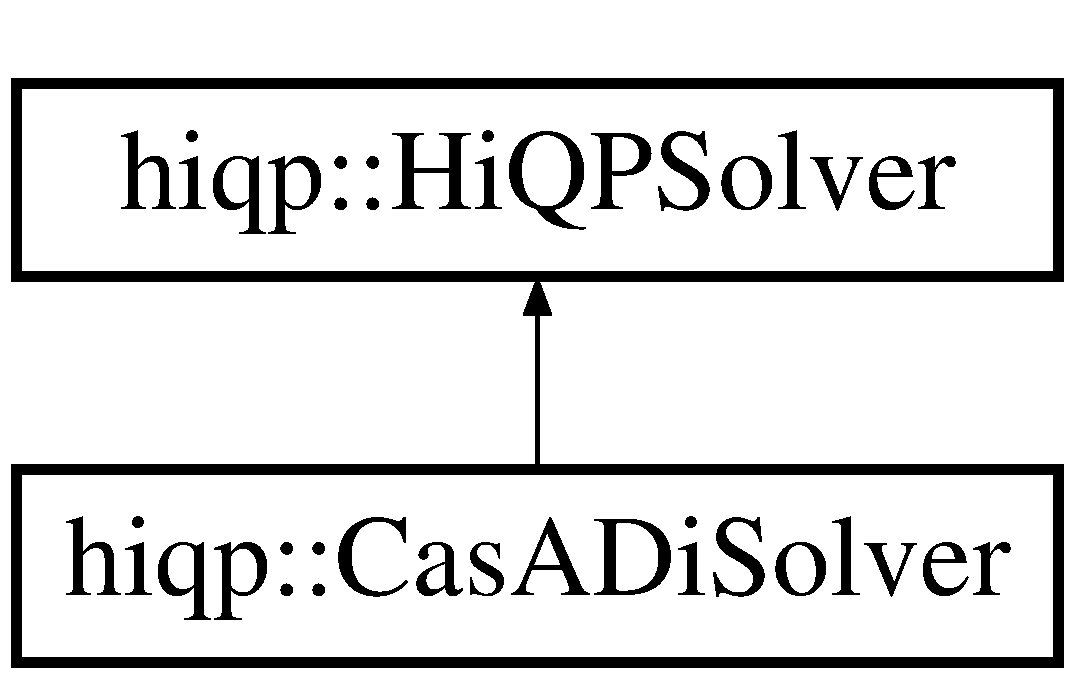
\includegraphics[height=2.000000cm]{classhiqp_1_1CasADiSolver}
\end{center}
\end{figure}
\subsection*{Public Member Functions}
\begin{DoxyCompactItemize}
\item 
\hypertarget{classhiqp_1_1CasADiSolver_a30fdfd2289613a3d38fd44a7db266134}{int {\bfseries solve} (std\-::vector$<$ double $>$ \&solution)}\label{classhiqp_1_1CasADiSolver_a30fdfd2289613a3d38fd44a7db266134}

\end{DoxyCompactItemize}
\subsection*{Additional Inherited Members}


The documentation for this class was generated from the following files\-:\begin{DoxyCompactItemize}
\item 
include/hiqp/solvers/\hyperlink{casadi__solver_8h}{casadi\-\_\-solver.\-h}\item 
src/solvers/casadi\-\_\-solver.\-cpp\end{DoxyCompactItemize}

\hypertarget{classhiqp_1_1DynamicsFirstOrder}{\section{hiqp\-:\-:Dynamics\-First\-Order Class Reference}
\label{classhiqp_1_1DynamicsFirstOrder}\index{hiqp\-::\-Dynamics\-First\-Order@{hiqp\-::\-Dynamics\-First\-Order}}
}


A general first-\/order task dynamics implementation that enforces an exponential decay of the task function value.  




{\ttfamily \#include $<$dynamics\-\_\-first\-\_\-order.\-h$>$}

Inheritance diagram for hiqp\-:\-:Dynamics\-First\-Order\-:\begin{figure}[H]
\begin{center}
\leavevmode
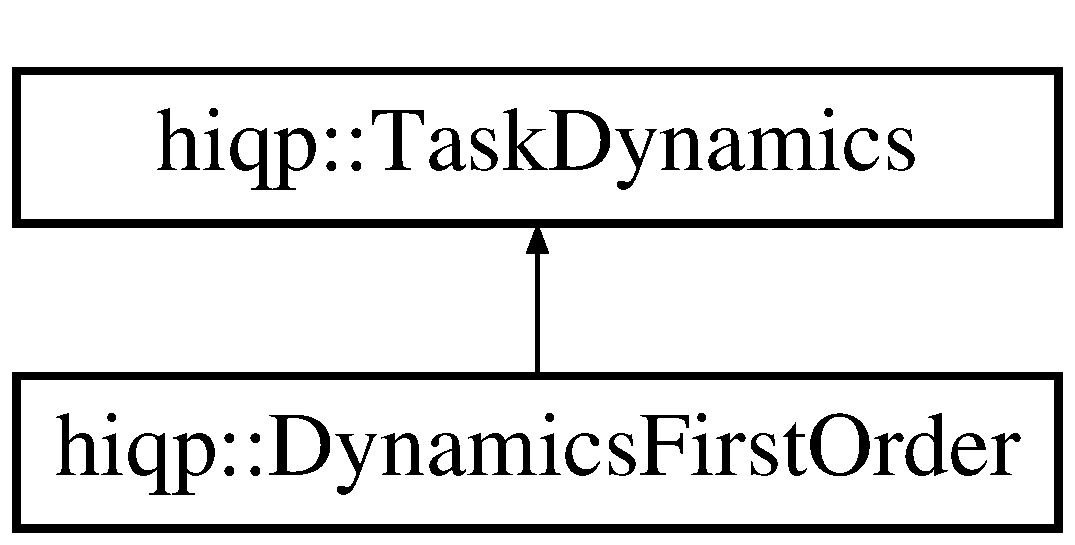
\includegraphics[height=2.000000cm]{classhiqp_1_1DynamicsFirstOrder}
\end{center}
\end{figure}
\subsection*{Public Member Functions}
\begin{DoxyCompactItemize}
\item 
\hypertarget{classhiqp_1_1DynamicsFirstOrder_ad88c60190ac28f11cd8919070a8f3be3}{int {\bfseries init} (const \hyperlink{classhiqp_1_1HiQPTimePoint}{Hi\-Q\-P\-Time\-Point} \&sampling\-\_\-time, const std\-::vector$<$ std\-::string $>$ \&parameters, const Eigen\-::\-Vector\-Xd \&e\-\_\-initial, const Eigen\-::\-Vector\-Xd \&e\-\_\-final)}\label{classhiqp_1_1DynamicsFirstOrder_ad88c60190ac28f11cd8919070a8f3be3}

\item 
\hypertarget{classhiqp_1_1DynamicsFirstOrder_ae4496d42170a20c473d3e6a378cd2378}{int {\bfseries apply} (const \hyperlink{classhiqp_1_1HiQPTimePoint}{Hi\-Q\-P\-Time\-Point} \&sampling\-\_\-time, const Eigen\-::\-Vector\-Xd \&e, const Eigen\-::\-Matrix\-Xd \&J, Eigen\-::\-Vector\-Xd \&e\-\_\-dot\-\_\-star)}\label{classhiqp_1_1DynamicsFirstOrder_ae4496d42170a20c473d3e6a378cd2378}

\item 
\hypertarget{classhiqp_1_1DynamicsFirstOrder_ae0be939fb0e31fdc0a7e3736f5e332e3}{int {\bfseries monitor} ()}\label{classhiqp_1_1DynamicsFirstOrder_ae0be939fb0e31fdc0a7e3736f5e332e3}

\end{DoxyCompactItemize}
\subsection*{Additional Inherited Members}


\subsection{Detailed Description}
A general first-\/order task dynamics implementation that enforces an exponential decay of the task function value. 

The documentation for this class was generated from the following files\-:\begin{DoxyCompactItemize}
\item 
include/hiqp/tasks/\hyperlink{dynamics__first__order_8h}{dynamics\-\_\-first\-\_\-order.\-h}\item 
src/tasks/\hyperlink{dynamics__first__order_8cpp}{dynamics\-\_\-first\-\_\-order.\-cpp}\end{DoxyCompactItemize}

\hypertarget{classhiqp_1_1DynamicsJntLimits}{\section{hiqp\-:\-:Dynamics\-Jnt\-Limits Class Reference}
\label{classhiqp_1_1DynamicsJntLimits}\index{hiqp\-::\-Dynamics\-Jnt\-Limits@{hiqp\-::\-Dynamics\-Jnt\-Limits}}
}
Inheritance diagram for hiqp\-:\-:Dynamics\-Jnt\-Limits\-:\begin{figure}[H]
\begin{center}
\leavevmode
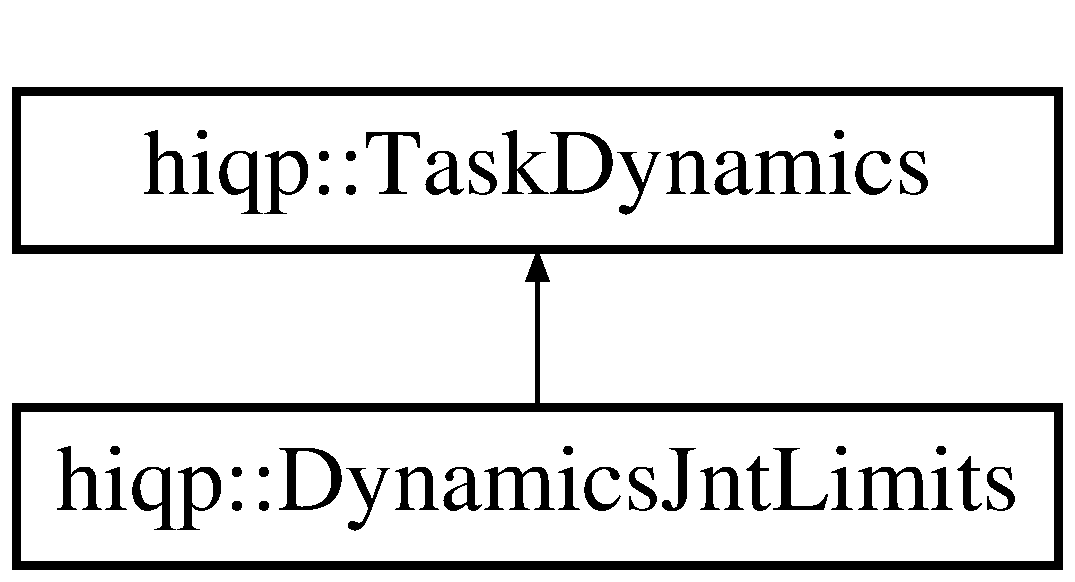
\includegraphics[height=2.000000cm]{classhiqp_1_1DynamicsJntLimits}
\end{center}
\end{figure}
\subsection*{Public Member Functions}
\begin{DoxyCompactItemize}
\item 
\hypertarget{classhiqp_1_1DynamicsJntLimits_aca0cb3a30a1d071e4cd958737e45cd26}{int {\bfseries init} (const \hyperlink{classhiqp_1_1HiQPTimePoint}{Hi\-Q\-P\-Time\-Point} \&sampling\-\_\-time, const std\-::vector$<$ std\-::string $>$ \&parameters, const Eigen\-::\-Vector\-Xd \&e\-\_\-initial, const Eigen\-::\-Vector\-Xd \&e\-\_\-final)}\label{classhiqp_1_1DynamicsJntLimits_aca0cb3a30a1d071e4cd958737e45cd26}

\item 
\hypertarget{classhiqp_1_1DynamicsJntLimits_a881943d401858f2c43134e96ee65b4e9}{int {\bfseries apply} (const \hyperlink{classhiqp_1_1HiQPTimePoint}{Hi\-Q\-P\-Time\-Point} \&sampling\-\_\-time, const Eigen\-::\-Vector\-Xd \&e, const Eigen\-::\-Matrix\-Xd \&J, Eigen\-::\-Vector\-Xd \&e\-\_\-dot\-\_\-star)}\label{classhiqp_1_1DynamicsJntLimits_a881943d401858f2c43134e96ee65b4e9}

\item 
\hypertarget{classhiqp_1_1DynamicsJntLimits_a65cdb43f439c451ca9279cfdc8ea6dc8}{int {\bfseries monitor} ()}\label{classhiqp_1_1DynamicsJntLimits_a65cdb43f439c451ca9279cfdc8ea6dc8}

\end{DoxyCompactItemize}
\subsection*{Additional Inherited Members}


The documentation for this class was generated from the following files\-:\begin{DoxyCompactItemize}
\item 
include/hiqp/tasks/\hyperlink{dynamics__jnt__limits_8h}{dynamics\-\_\-jnt\-\_\-limits.\-h}\item 
src/tasks/\hyperlink{dynamics__jnt__limits_8cpp}{dynamics\-\_\-jnt\-\_\-limits.\-cpp}\end{DoxyCompactItemize}

\hypertarget{classhiqp_1_1DynamicsMinimalJerk}{\section{hiqp\-:\-:Dynamics\-Minimal\-Jerk Class Reference}
\label{classhiqp_1_1DynamicsMinimalJerk}\index{hiqp\-::\-Dynamics\-Minimal\-Jerk@{hiqp\-::\-Dynamics\-Minimal\-Jerk}}
}
Inheritance diagram for hiqp\-:\-:Dynamics\-Minimal\-Jerk\-:\begin{figure}[H]
\begin{center}
\leavevmode
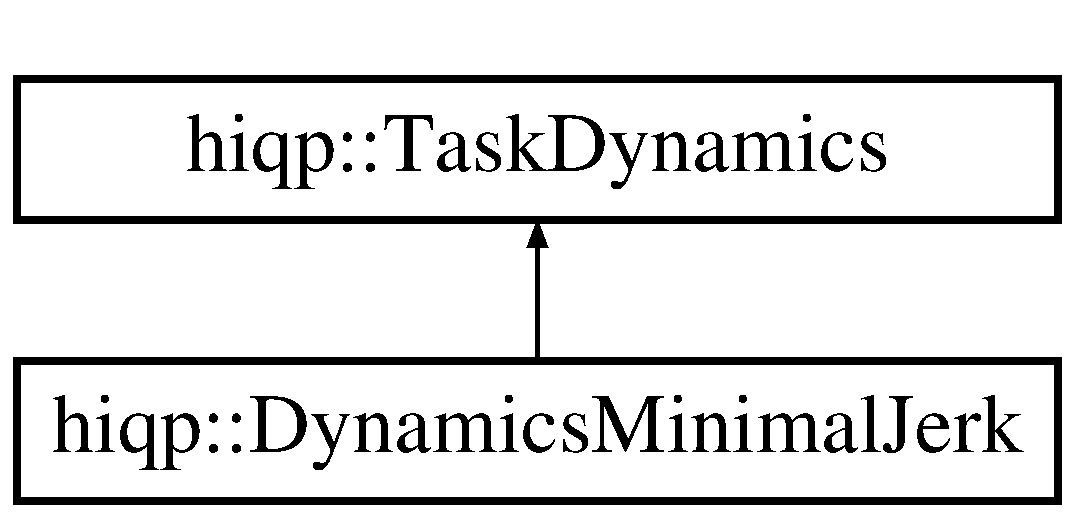
\includegraphics[height=2.000000cm]{classhiqp_1_1DynamicsMinimalJerk}
\end{center}
\end{figure}
\subsection*{Public Member Functions}
\begin{DoxyCompactItemize}
\item 
\hypertarget{classhiqp_1_1DynamicsMinimalJerk_a8e29102ccfbaed3cdfcc965d3e1fcd7a}{int {\bfseries init} (const \hyperlink{classhiqp_1_1HiQPTimePoint}{Hi\-Q\-P\-Time\-Point} \&sampling\-\_\-time, const std\-::vector$<$ std\-::string $>$ \&parameters, const Eigen\-::\-Vector\-Xd \&e\-\_\-initial, const Eigen\-::\-Vector\-Xd \&e\-\_\-final)}\label{classhiqp_1_1DynamicsMinimalJerk_a8e29102ccfbaed3cdfcc965d3e1fcd7a}

\item 
\hypertarget{classhiqp_1_1DynamicsMinimalJerk_a275c96acdb50b0ff70a026352868b616}{int {\bfseries apply} (const \hyperlink{classhiqp_1_1HiQPTimePoint}{Hi\-Q\-P\-Time\-Point} \&sampling\-\_\-time, const Eigen\-::\-Vector\-Xd \&e, const Eigen\-::\-Matrix\-Xd \&J, Eigen\-::\-Vector\-Xd \&e\-\_\-dot\-\_\-star)}\label{classhiqp_1_1DynamicsMinimalJerk_a275c96acdb50b0ff70a026352868b616}

\item 
\hypertarget{classhiqp_1_1DynamicsMinimalJerk_a05e1d6c10f9f7f896f653b287f8192b1}{int {\bfseries monitor} ()}\label{classhiqp_1_1DynamicsMinimalJerk_a05e1d6c10f9f7f896f653b287f8192b1}

\end{DoxyCompactItemize}
\subsection*{Additional Inherited Members}


The documentation for this class was generated from the following files\-:\begin{DoxyCompactItemize}
\item 
include/hiqp/tasks/\hyperlink{dynamics__minimal__jerk_8h}{dynamics\-\_\-minimal\-\_\-jerk.\-h}\item 
src/tasks/\hyperlink{dynamics__minimal__jerk_8cpp}{dynamics\-\_\-minimal\-\_\-jerk.\-cpp}\end{DoxyCompactItemize}

\hypertarget{classhiqp_1_1geometric__primitives_1_1GeometricBox}{\section{hiqp\-:\-:geometric\-\_\-primitives\-:\-:Geometric\-Box Class Reference}
\label{classhiqp_1_1geometric__primitives_1_1GeometricBox}\index{hiqp\-::geometric\-\_\-primitives\-::\-Geometric\-Box@{hiqp\-::geometric\-\_\-primitives\-::\-Geometric\-Box}}
}


Parameters\-:\par
 \mbox{[}c.\-x, c.\-y, c.\-z, dim.\-x, dim.\-y, dim.\-z\mbox{]} \par
 \mbox{[}c.\-x, c.\-y, c.\-z, dim.\-x, dim.\-y, dim.\-z, angle.\-x, angle.\-y, angle.\-z\mbox{]} \par
 \mbox{[}c.\-x, c.\-y, c.\-z, dim.\-x, dim.\-y, dim.\-z, q.\-w, q.\-x, q.\-y, q.\-z\mbox{]} \par
  




{\ttfamily \#include $<$geometric\-\_\-box.\-h$>$}

Inheritance diagram for hiqp\-:\-:geometric\-\_\-primitives\-:\-:Geometric\-Box\-:\begin{figure}[H]
\begin{center}
\leavevmode
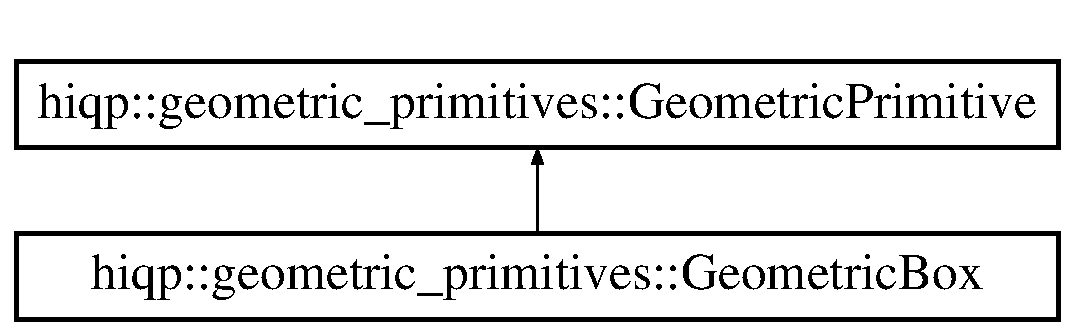
\includegraphics[height=2.000000cm]{classhiqp_1_1geometric__primitives_1_1GeometricBox}
\end{center}
\end{figure}
\subsection*{Public Member Functions}
\begin{DoxyCompactItemize}
\item 
\hypertarget{classhiqp_1_1geometric__primitives_1_1GeometricBox_aa52d023049089c48fe4d58e1abda191e}{{\bfseries Geometric\-Box} (const std\-::string \&name, const std\-::string \&frame\-\_\-id, bool visible, const std\-::vector$<$ double $>$ \&color)}\label{classhiqp_1_1geometric__primitives_1_1GeometricBox_aa52d023049089c48fe4d58e1abda191e}

\item 
int \hyperlink{classhiqp_1_1geometric__primitives_1_1GeometricBox_aae7d637b515e2b35c901a7e2fb5dd6cd}{init} (const std\-::vector$<$ double $>$ \&parameters)
\begin{DoxyCompactList}\small\item\em Parses a set of parameters and initializes the box. \end{DoxyCompactList}\item 
\hypertarget{classhiqp_1_1geometric__primitives_1_1GeometricBox_acfb9b2388e5219895e5d5818fc0309d9}{const K\-D\-L\-::\-Vector \& {\bfseries get\-Center\-K\-D\-L} ()}\label{classhiqp_1_1geometric__primitives_1_1GeometricBox_acfb9b2388e5219895e5d5818fc0309d9}

\item 
\hypertarget{classhiqp_1_1geometric__primitives_1_1GeometricBox_a419fd54ee9d68557fde580047d674d2a}{const Eigen\-::\-Vector3d \& {\bfseries get\-Center\-Eigen} ()}\label{classhiqp_1_1geometric__primitives_1_1GeometricBox_a419fd54ee9d68557fde580047d674d2a}

\item 
\hypertarget{classhiqp_1_1geometric__primitives_1_1GeometricBox_a25e529e27e5cf1ea193f09b6a3c52e38}{const K\-D\-L\-::\-Vector \& {\bfseries get\-Dimensions\-K\-D\-L} ()}\label{classhiqp_1_1geometric__primitives_1_1GeometricBox_a25e529e27e5cf1ea193f09b6a3c52e38}

\item 
\hypertarget{classhiqp_1_1geometric__primitives_1_1GeometricBox_a77f1de122e7860e9951efb118287765b}{const Eigen\-::\-Vector3d \& {\bfseries get\-Dimensions\-Eigen} ()}\label{classhiqp_1_1geometric__primitives_1_1GeometricBox_a77f1de122e7860e9951efb118287765b}

\item 
\hypertarget{classhiqp_1_1geometric__primitives_1_1GeometricBox_ab1e112b2af3cc6982a742ee641056bfb}{const Eigen\-::\-Quaternion$<$ double $>$ \& {\bfseries get\-Quaternion\-Eigen} ()}\label{classhiqp_1_1geometric__primitives_1_1GeometricBox_ab1e112b2af3cc6982a742ee641056bfb}

\item 
\hypertarget{classhiqp_1_1geometric__primitives_1_1GeometricBox_ad92b80f4b613257574f8fe178e9bb329}{void {\bfseries get\-Quaternion} (double \&w, double \&x, double \&y, double \&z)}\label{classhiqp_1_1geometric__primitives_1_1GeometricBox_ad92b80f4b613257574f8fe178e9bb329}

\item 
\hypertarget{classhiqp_1_1geometric__primitives_1_1GeometricBox_acd1f99817d10aa2765498322fb503c09}{const Eigen\-::\-Matrix3d \& {\bfseries get\-Scaling\-Matrix} ()}\label{classhiqp_1_1geometric__primitives_1_1GeometricBox_acd1f99817d10aa2765498322fb503c09}

\item 
\hypertarget{classhiqp_1_1geometric__primitives_1_1GeometricBox_adbfbd7788959ac285a96e5eff56a5c61}{double {\bfseries get\-Center\-X} ()}\label{classhiqp_1_1geometric__primitives_1_1GeometricBox_adbfbd7788959ac285a96e5eff56a5c61}

\item 
\hypertarget{classhiqp_1_1geometric__primitives_1_1GeometricBox_a9cdcda87654088a51bc821b67ce88942}{double {\bfseries get\-Center\-Y} ()}\label{classhiqp_1_1geometric__primitives_1_1GeometricBox_a9cdcda87654088a51bc821b67ce88942}

\item 
\hypertarget{classhiqp_1_1geometric__primitives_1_1GeometricBox_ab4c3f4453b9167e2f82fff1b236a95d7}{double {\bfseries get\-Center\-Z} ()}\label{classhiqp_1_1geometric__primitives_1_1GeometricBox_ab4c3f4453b9167e2f82fff1b236a95d7}

\item 
\hypertarget{classhiqp_1_1geometric__primitives_1_1GeometricBox_a8f5ccb354be710855b20adb54bf207f3}{double {\bfseries get\-Dim\-X} ()}\label{classhiqp_1_1geometric__primitives_1_1GeometricBox_a8f5ccb354be710855b20adb54bf207f3}

\item 
\hypertarget{classhiqp_1_1geometric__primitives_1_1GeometricBox_a954412b5c06750258d5250ae1c206622}{double {\bfseries get\-Dim\-Y} ()}\label{classhiqp_1_1geometric__primitives_1_1GeometricBox_a954412b5c06750258d5250ae1c206622}

\item 
\hypertarget{classhiqp_1_1geometric__primitives_1_1GeometricBox_a07282003e93d457b36e5d09a6774f2c9}{double {\bfseries get\-Dim\-Z} ()}\label{classhiqp_1_1geometric__primitives_1_1GeometricBox_a07282003e93d457b36e5d09a6774f2c9}

\end{DoxyCompactItemize}
\subsection*{Protected Attributes}
\begin{DoxyCompactItemize}
\item 
\hypertarget{classhiqp_1_1geometric__primitives_1_1GeometricBox_ad9b5e3a8dcc30620584bf27d6d1dda71}{K\-D\-L\-::\-Vector {\bfseries kdl\-\_\-c\-\_\-}}\label{classhiqp_1_1geometric__primitives_1_1GeometricBox_ad9b5e3a8dcc30620584bf27d6d1dda71}

\item 
\hypertarget{classhiqp_1_1geometric__primitives_1_1GeometricBox_a96ad47d72a6dbf78c4f52db15a52ed01}{Eigen\-::\-Vector3d {\bfseries eigen\-\_\-c\-\_\-}}\label{classhiqp_1_1geometric__primitives_1_1GeometricBox_a96ad47d72a6dbf78c4f52db15a52ed01}

\item 
\hypertarget{classhiqp_1_1geometric__primitives_1_1GeometricBox_aa4bd006daadaa6feed4fd24c1892629a}{K\-D\-L\-::\-Vector {\bfseries kdl\-\_\-dim\-\_\-}}\label{classhiqp_1_1geometric__primitives_1_1GeometricBox_aa4bd006daadaa6feed4fd24c1892629a}

\item 
\hypertarget{classhiqp_1_1geometric__primitives_1_1GeometricBox_a8be3b55e5793038692a7f43663b97309}{Eigen\-::\-Vector3d {\bfseries eigen\-\_\-dim\-\_\-}}\label{classhiqp_1_1geometric__primitives_1_1GeometricBox_a8be3b55e5793038692a7f43663b97309}

\item 
\hypertarget{classhiqp_1_1geometric__primitives_1_1GeometricBox_a4a57c7bef7efb4ed2f5535c796b00678}{Eigen\-::\-Quaternion$<$ double $>$ {\bfseries q\-\_\-}}\label{classhiqp_1_1geometric__primitives_1_1GeometricBox_a4a57c7bef7efb4ed2f5535c796b00678}

\item 
\hypertarget{classhiqp_1_1geometric__primitives_1_1GeometricBox_a6889ebbde5629bcd835a63948a3062b8}{Eigen\-::\-Matrix3d {\bfseries scaling\-\_\-matrix\-\_\-}}\label{classhiqp_1_1geometric__primitives_1_1GeometricBox_a6889ebbde5629bcd835a63948a3062b8}

\end{DoxyCompactItemize}


\subsection{Detailed Description}
Parameters\-:\par
 \mbox{[}c.\-x, c.\-y, c.\-z, dim.\-x, dim.\-y, dim.\-z\mbox{]} \par
 \mbox{[}c.\-x, c.\-y, c.\-z, dim.\-x, dim.\-y, dim.\-z, angle.\-x, angle.\-y, angle.\-z\mbox{]} \par
 \mbox{[}c.\-x, c.\-y, c.\-z, dim.\-x, dim.\-y, dim.\-z, q.\-w, q.\-x, q.\-y, q.\-z\mbox{]} \par
 

\subsection{Member Function Documentation}
\hypertarget{classhiqp_1_1geometric__primitives_1_1GeometricBox_aae7d637b515e2b35c901a7e2fb5dd6cd}{\index{hiqp\-::geometric\-\_\-primitives\-::\-Geometric\-Box@{hiqp\-::geometric\-\_\-primitives\-::\-Geometric\-Box}!init@{init}}
\index{init@{init}!hiqp::geometric_primitives::GeometricBox@{hiqp\-::geometric\-\_\-primitives\-::\-Geometric\-Box}}
\subsubsection[{init}]{\setlength{\rightskip}{0pt plus 5cm}int hiqp\-::geometric\-\_\-primitives\-::\-Geometric\-Box\-::init (
\begin{DoxyParamCaption}
\item[{const std\-::vector$<$ double $>$ \&}]{parameters}
\end{DoxyParamCaption}
)\hspace{0.3cm}{\ttfamily [inline]}, {\ttfamily [virtual]}}}\label{classhiqp_1_1geometric__primitives_1_1GeometricBox_aae7d637b515e2b35c901a7e2fb5dd6cd}


Parses a set of parameters and initializes the box. 


\begin{DoxyParams}{Parameters}
{\em parameters} & should be of size 6, 9, or 10. \par
 Indices 0-\/2 (required) defines the position of the center of the box, \par
 indices 3-\/5 (required) defines the dimensions of the box, \par
 indices 6-\/8 (optional) defines euler angles of the orientation of the box (xyz) \par
 indices 6-\/9 (optional) defines a quaternion for the orientation of the box.\\
\hline
\end{DoxyParams}
\begin{DoxyReturn}{Returns}
0 on success, -\/1 if the wrong number of parameters was sent 
\end{DoxyReturn}


Implements \hyperlink{classhiqp_1_1geometric__primitives_1_1GeometricPrimitive_a3697e5afb0121715280da649b8bd711d}{hiqp\-::geometric\-\_\-primitives\-::\-Geometric\-Primitive}.



The documentation for this class was generated from the following file\-:\begin{DoxyCompactItemize}
\item 
include/hiqp/geometric\-\_\-primitives/geometric\-\_\-box.\-h\end{DoxyCompactItemize}

\hypertarget{classhiqp_1_1geometric__primitives_1_1GeometricCylinder}{\section{hiqp\-:\-:geometric\-\_\-primitives\-:\-:Geometric\-Cylinder Class Reference}
\label{classhiqp_1_1geometric__primitives_1_1GeometricCylinder}\index{hiqp\-::geometric\-\_\-primitives\-::\-Geometric\-Cylinder@{hiqp\-::geometric\-\_\-primitives\-::\-Geometric\-Cylinder}}
}


Parameters\-: \mbox{[}dir.\-x, dir.\-y, dir.\-z, offset.\-x, offset.\-y, offset.\-z, radius, height\mbox{]}.  




{\ttfamily \#include $<$geometric\-\_\-cylinder.\-h$>$}

Inheritance diagram for hiqp\-:\-:geometric\-\_\-primitives\-:\-:Geometric\-Cylinder\-:\begin{figure}[H]
\begin{center}
\leavevmode
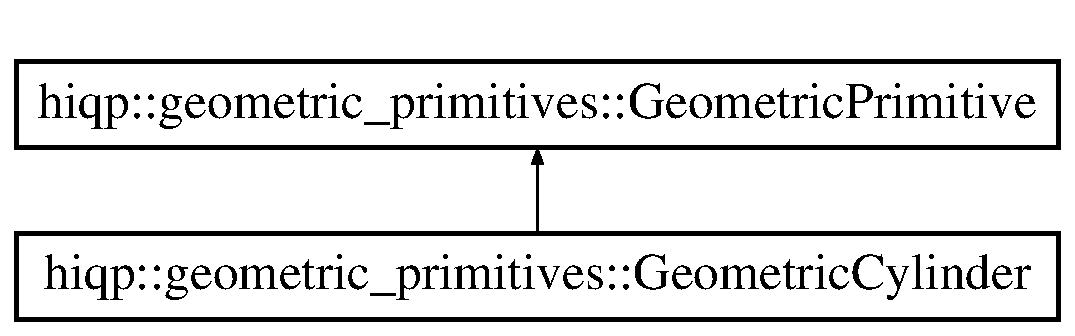
\includegraphics[height=2.000000cm]{classhiqp_1_1geometric__primitives_1_1GeometricCylinder}
\end{center}
\end{figure}
\subsection*{Public Member Functions}
\begin{DoxyCompactItemize}
\item 
\hypertarget{classhiqp_1_1geometric__primitives_1_1GeometricCylinder_af597b83669074eaf0eeb984fb6a90da6}{{\bfseries Geometric\-Cylinder} (const std\-::string \&name, const std\-::string \&frame\-\_\-id, bool visible, const std\-::vector$<$ double $>$ \&color)}\label{classhiqp_1_1geometric__primitives_1_1GeometricCylinder_af597b83669074eaf0eeb984fb6a90da6}

\item 
int \hyperlink{classhiqp_1_1geometric__primitives_1_1GeometricCylinder_aa3a355a12068bfd1b51e3ea07b08e469}{init} (const std\-::vector$<$ double $>$ \&parameters)
\begin{DoxyCompactList}\small\item\em Parses a set of parameters and initializes the cylinder. \end{DoxyCompactList}\item 
\hypertarget{classhiqp_1_1geometric__primitives_1_1GeometricCylinder_a91a05ff0aea792fcb0d94f3a9c17c8ed}{const K\-D\-L\-::\-Vector \& {\bfseries get\-Direction\-K\-D\-L} ()}\label{classhiqp_1_1geometric__primitives_1_1GeometricCylinder_a91a05ff0aea792fcb0d94f3a9c17c8ed}

\item 
\hypertarget{classhiqp_1_1geometric__primitives_1_1GeometricCylinder_a91c16962324b4ffefd6b1ff3eaf2c29b}{const Eigen\-::\-Vector3d \& {\bfseries get\-Direction\-Eigen} ()}\label{classhiqp_1_1geometric__primitives_1_1GeometricCylinder_a91c16962324b4ffefd6b1ff3eaf2c29b}

\item 
\hypertarget{classhiqp_1_1geometric__primitives_1_1GeometricCylinder_a8cce11af002bf3efb3239050e3928bb9}{const K\-D\-L\-::\-Vector \& {\bfseries get\-Offset\-K\-D\-L} ()}\label{classhiqp_1_1geometric__primitives_1_1GeometricCylinder_a8cce11af002bf3efb3239050e3928bb9}

\item 
\hypertarget{classhiqp_1_1geometric__primitives_1_1GeometricCylinder_a9a298067229c935701638410b24ff0f2}{const Eigen\-::\-Vector3d \& {\bfseries get\-Offset\-Eigen} ()}\label{classhiqp_1_1geometric__primitives_1_1GeometricCylinder_a9a298067229c935701638410b24ff0f2}

\item 
\hypertarget{classhiqp_1_1geometric__primitives_1_1GeometricCylinder_a78645047ee5004b0f1f30a5eb5be7654}{double {\bfseries get\-Height} ()}\label{classhiqp_1_1geometric__primitives_1_1GeometricCylinder_a78645047ee5004b0f1f30a5eb5be7654}

\item 
\hypertarget{classhiqp_1_1geometric__primitives_1_1GeometricCylinder_ab1a7573392a5ead7eea74c143c6fe953}{double {\bfseries get\-Radius} ()}\label{classhiqp_1_1geometric__primitives_1_1GeometricCylinder_ab1a7573392a5ead7eea74c143c6fe953}

\item 
\hypertarget{classhiqp_1_1geometric__primitives_1_1GeometricCylinder_ae670d2424f428140986ba7ca2c84f87d}{bool {\bfseries is\-Infinite} ()}\label{classhiqp_1_1geometric__primitives_1_1GeometricCylinder_ae670d2424f428140986ba7ca2c84f87d}

\item 
\hypertarget{classhiqp_1_1geometric__primitives_1_1GeometricCylinder_ad435a59b651f37f1e83b4d40bd52a93f}{double {\bfseries get\-Direction\-X} ()}\label{classhiqp_1_1geometric__primitives_1_1GeometricCylinder_ad435a59b651f37f1e83b4d40bd52a93f}

\item 
\hypertarget{classhiqp_1_1geometric__primitives_1_1GeometricCylinder_a83fcee513ee5f0baf50932cc4d247652}{double {\bfseries get\-Direction\-Y} ()}\label{classhiqp_1_1geometric__primitives_1_1GeometricCylinder_a83fcee513ee5f0baf50932cc4d247652}

\item 
\hypertarget{classhiqp_1_1geometric__primitives_1_1GeometricCylinder_a19cec2f53c14f9336a90997891eba5f6}{double {\bfseries get\-Direction\-Z} ()}\label{classhiqp_1_1geometric__primitives_1_1GeometricCylinder_a19cec2f53c14f9336a90997891eba5f6}

\item 
\hypertarget{classhiqp_1_1geometric__primitives_1_1GeometricCylinder_a08d2aa46ce321c6cd90484303e6e4ba6}{double {\bfseries get\-Offset\-X} ()}\label{classhiqp_1_1geometric__primitives_1_1GeometricCylinder_a08d2aa46ce321c6cd90484303e6e4ba6}

\item 
\hypertarget{classhiqp_1_1geometric__primitives_1_1GeometricCylinder_a4a87620bc7eef750b99246785d2c86de}{double {\bfseries get\-Offset\-Y} ()}\label{classhiqp_1_1geometric__primitives_1_1GeometricCylinder_a4a87620bc7eef750b99246785d2c86de}

\item 
\hypertarget{classhiqp_1_1geometric__primitives_1_1GeometricCylinder_a17f8ff59870cf55fe2a5811366a2075d}{double {\bfseries get\-Offset\-Z} ()}\label{classhiqp_1_1geometric__primitives_1_1GeometricCylinder_a17f8ff59870cf55fe2a5811366a2075d}

\end{DoxyCompactItemize}
\subsection*{Protected Attributes}
\begin{DoxyCompactItemize}
\item 
\hypertarget{classhiqp_1_1geometric__primitives_1_1GeometricCylinder_a4f14ff073aadefec06d354e5a4aa6a02}{K\-D\-L\-::\-Vector {\bfseries kdl\-\_\-v\-\_\-}}\label{classhiqp_1_1geometric__primitives_1_1GeometricCylinder_a4f14ff073aadefec06d354e5a4aa6a02}

\item 
\hypertarget{classhiqp_1_1geometric__primitives_1_1GeometricCylinder_a4f1ecaa9cb967a92875ba90ba5ee16cd}{Eigen\-::\-Vector3d {\bfseries eigen\-\_\-v\-\_\-}}\label{classhiqp_1_1geometric__primitives_1_1GeometricCylinder_a4f1ecaa9cb967a92875ba90ba5ee16cd}

\item 
\hypertarget{classhiqp_1_1geometric__primitives_1_1GeometricCylinder_af31a991daf4defbb80dad9a4ce7ffbe8}{K\-D\-L\-::\-Vector {\bfseries kdl\-\_\-p\-\_\-}}\label{classhiqp_1_1geometric__primitives_1_1GeometricCylinder_af31a991daf4defbb80dad9a4ce7ffbe8}

\item 
\hypertarget{classhiqp_1_1geometric__primitives_1_1GeometricCylinder_a0acb0c1f78254b5d05119192db73b364}{Eigen\-::\-Vector3d {\bfseries eigen\-\_\-p\-\_\-}}\label{classhiqp_1_1geometric__primitives_1_1GeometricCylinder_a0acb0c1f78254b5d05119192db73b364}

\item 
\hypertarget{classhiqp_1_1geometric__primitives_1_1GeometricCylinder_adf639620c8c52f76b999fcacb4191a68}{double {\bfseries h\-\_\-}}\label{classhiqp_1_1geometric__primitives_1_1GeometricCylinder_adf639620c8c52f76b999fcacb4191a68}

\item 
\hypertarget{classhiqp_1_1geometric__primitives_1_1GeometricCylinder_afa05dbc48e949a494aa3281e239bed73}{double {\bfseries radius\-\_\-}}\label{classhiqp_1_1geometric__primitives_1_1GeometricCylinder_afa05dbc48e949a494aa3281e239bed73}

\end{DoxyCompactItemize}


\subsection{Detailed Description}
Parameters\-: \mbox{[}dir.\-x, dir.\-y, dir.\-z, offset.\-x, offset.\-y, offset.\-z, radius, height\mbox{]}. 

\subsection{Member Function Documentation}
\hypertarget{classhiqp_1_1geometric__primitives_1_1GeometricCylinder_aa3a355a12068bfd1b51e3ea07b08e469}{\index{hiqp\-::geometric\-\_\-primitives\-::\-Geometric\-Cylinder@{hiqp\-::geometric\-\_\-primitives\-::\-Geometric\-Cylinder}!init@{init}}
\index{init@{init}!hiqp::geometric_primitives::GeometricCylinder@{hiqp\-::geometric\-\_\-primitives\-::\-Geometric\-Cylinder}}
\subsubsection[{init}]{\setlength{\rightskip}{0pt plus 5cm}int hiqp\-::geometric\-\_\-primitives\-::\-Geometric\-Cylinder\-::init (
\begin{DoxyParamCaption}
\item[{const std\-::vector$<$ double $>$ \&}]{parameters}
\end{DoxyParamCaption}
)\hspace{0.3cm}{\ttfamily [inline]}, {\ttfamily [virtual]}}}\label{classhiqp_1_1geometric__primitives_1_1GeometricCylinder_aa3a355a12068bfd1b51e3ea07b08e469}


Parses a set of parameters and initializes the cylinder. 


\begin{DoxyParams}{Parameters}
{\em parameters} & should be of size 8. \par
 Indices 0-\/2 (required) defines the directional vector of the cylinder, \par
 indices 3-\/5 (required) defines the position of a point on the cylinder's coaxial line, \par
 index 6 (required) defines the radius of the cylinder, \par
 index 7 (required) defines the height of the cylinder.\\
\hline
\end{DoxyParams}
\begin{DoxyReturn}{Returns}
0 on success, -\/1 if the wrong number of parameters was sent 
\end{DoxyReturn}


Implements \hyperlink{classhiqp_1_1geometric__primitives_1_1GeometricPrimitive_a3697e5afb0121715280da649b8bd711d}{hiqp\-::geometric\-\_\-primitives\-::\-Geometric\-Primitive}.



The documentation for this class was generated from the following file\-:\begin{DoxyCompactItemize}
\item 
include/hiqp/geometric\-\_\-primitives/geometric\-\_\-cylinder.\-h\end{DoxyCompactItemize}

\hypertarget{classhiqp_1_1geometric__primitives_1_1GeometricLine}{\section{hiqp\-:\-:geometric\-\_\-primitives\-:\-:Geometric\-Line Class Reference}
\label{classhiqp_1_1geometric__primitives_1_1GeometricLine}\index{hiqp\-::geometric\-\_\-primitives\-::\-Geometric\-Line@{hiqp\-::geometric\-\_\-primitives\-::\-Geometric\-Line}}
}


Parameters\-: \mbox{[}dir.\-x, dir.\-y, dir.\-z, offset.\-x, offset.\-y, offset.\-z\mbox{]}.  




{\ttfamily \#include $<$geometric\-\_\-line.\-h$>$}

Inheritance diagram for hiqp\-:\-:geometric\-\_\-primitives\-:\-:Geometric\-Line\-:\begin{figure}[H]
\begin{center}
\leavevmode
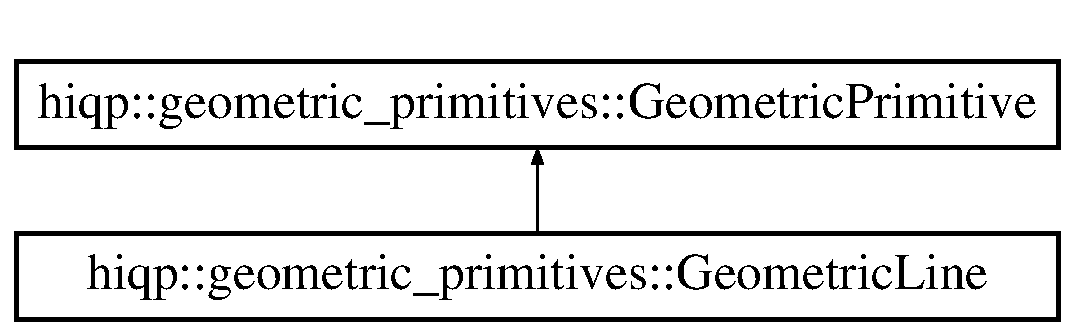
\includegraphics[height=2.000000cm]{classhiqp_1_1geometric__primitives_1_1GeometricLine}
\end{center}
\end{figure}
\subsection*{Public Member Functions}
\begin{DoxyCompactItemize}
\item 
\hypertarget{classhiqp_1_1geometric__primitives_1_1GeometricLine_a1f0ff1cd774363ef7a70095b066a4622}{{\bfseries Geometric\-Line} (const std\-::string \&name, const std\-::string \&frame\-\_\-id, bool visible, const std\-::vector$<$ double $>$ \&color)}\label{classhiqp_1_1geometric__primitives_1_1GeometricLine_a1f0ff1cd774363ef7a70095b066a4622}

\item 
int \hyperlink{classhiqp_1_1geometric__primitives_1_1GeometricLine_af6c0a5187fe9d298eaf2c8ef0637436f}{init} (const std\-::vector$<$ double $>$ \&parameters)
\begin{DoxyCompactList}\small\item\em Parses a set of parameters and initializes the line. \end{DoxyCompactList}\item 
\hypertarget{classhiqp_1_1geometric__primitives_1_1GeometricLine_a90b023a0126706d35719c9b9637915ba}{const K\-D\-L\-::\-Vector \& {\bfseries get\-Direction\-K\-D\-L} ()}\label{classhiqp_1_1geometric__primitives_1_1GeometricLine_a90b023a0126706d35719c9b9637915ba}

\item 
\hypertarget{classhiqp_1_1geometric__primitives_1_1GeometricLine_a66fe98ec0916331d12881f49cc4d9c69}{const Eigen\-::\-Vector3d \& {\bfseries get\-Direction\-Eigen} ()}\label{classhiqp_1_1geometric__primitives_1_1GeometricLine_a66fe98ec0916331d12881f49cc4d9c69}

\item 
\hypertarget{classhiqp_1_1geometric__primitives_1_1GeometricLine_abe8104c0a22ae25c1605fbafce4a28a9}{const K\-D\-L\-::\-Vector \& {\bfseries get\-Offset\-K\-D\-L} ()}\label{classhiqp_1_1geometric__primitives_1_1GeometricLine_abe8104c0a22ae25c1605fbafce4a28a9}

\item 
\hypertarget{classhiqp_1_1geometric__primitives_1_1GeometricLine_af454ca8815f308b7274b335b9f31c243}{const Eigen\-::\-Vector3d \& {\bfseries get\-Offset\-Eigen} ()}\label{classhiqp_1_1geometric__primitives_1_1GeometricLine_af454ca8815f308b7274b335b9f31c243}

\item 
\hypertarget{classhiqp_1_1geometric__primitives_1_1GeometricLine_a21cecdd031b36189ae2903751d2f0381}{bool {\bfseries is\-Infinite} ()}\label{classhiqp_1_1geometric__primitives_1_1GeometricLine_a21cecdd031b36189ae2903751d2f0381}

\item 
\hypertarget{classhiqp_1_1geometric__primitives_1_1GeometricLine_a79b3368b5d32da06586baeae50332064}{double {\bfseries get\-Direction\-X} ()}\label{classhiqp_1_1geometric__primitives_1_1GeometricLine_a79b3368b5d32da06586baeae50332064}

\item 
\hypertarget{classhiqp_1_1geometric__primitives_1_1GeometricLine_a0871efe61b83202f965924607296ba8e}{double {\bfseries get\-Direction\-Y} ()}\label{classhiqp_1_1geometric__primitives_1_1GeometricLine_a0871efe61b83202f965924607296ba8e}

\item 
\hypertarget{classhiqp_1_1geometric__primitives_1_1GeometricLine_a0c0fbdb1a69be7949b03e7808b0e003f}{double {\bfseries get\-Direction\-Z} ()}\label{classhiqp_1_1geometric__primitives_1_1GeometricLine_a0c0fbdb1a69be7949b03e7808b0e003f}

\item 
\hypertarget{classhiqp_1_1geometric__primitives_1_1GeometricLine_a9ce51f34c68a67b8c0e85fdf25d4916b}{double {\bfseries get\-Offset\-X} ()}\label{classhiqp_1_1geometric__primitives_1_1GeometricLine_a9ce51f34c68a67b8c0e85fdf25d4916b}

\item 
\hypertarget{classhiqp_1_1geometric__primitives_1_1GeometricLine_ab2eb6db0c441740a5e1724a4bb098449}{double {\bfseries get\-Offset\-Y} ()}\label{classhiqp_1_1geometric__primitives_1_1GeometricLine_ab2eb6db0c441740a5e1724a4bb098449}

\item 
\hypertarget{classhiqp_1_1geometric__primitives_1_1GeometricLine_ab832c44152fdec34b4071d21f86a3e06}{double {\bfseries get\-Offset\-Z} ()}\label{classhiqp_1_1geometric__primitives_1_1GeometricLine_ab832c44152fdec34b4071d21f86a3e06}

\end{DoxyCompactItemize}
\subsection*{Protected Attributes}
\begin{DoxyCompactItemize}
\item 
\hypertarget{classhiqp_1_1geometric__primitives_1_1GeometricLine_ad55d98c54189b4c91e2e968d7daf123d}{K\-D\-L\-::\-Vector {\bfseries kdl\-\_\-v\-\_\-}}\label{classhiqp_1_1geometric__primitives_1_1GeometricLine_ad55d98c54189b4c91e2e968d7daf123d}

\item 
\hypertarget{classhiqp_1_1geometric__primitives_1_1GeometricLine_aa84ecd396066feff7b3290b7c7178e32}{Eigen\-::\-Vector3d {\bfseries eigen\-\_\-v\-\_\-}}\label{classhiqp_1_1geometric__primitives_1_1GeometricLine_aa84ecd396066feff7b3290b7c7178e32}

\item 
\hypertarget{classhiqp_1_1geometric__primitives_1_1GeometricLine_a650defd742193255dc40eff0d3ff811f}{K\-D\-L\-::\-Vector {\bfseries kdl\-\_\-p\-\_\-}}\label{classhiqp_1_1geometric__primitives_1_1GeometricLine_a650defd742193255dc40eff0d3ff811f}

\item 
\hypertarget{classhiqp_1_1geometric__primitives_1_1GeometricLine_a56edbb80b40cfd1e672831bd9a637d44}{Eigen\-::\-Vector3d {\bfseries eigen\-\_\-p\-\_\-}}\label{classhiqp_1_1geometric__primitives_1_1GeometricLine_a56edbb80b40cfd1e672831bd9a637d44}

\item 
\hypertarget{classhiqp_1_1geometric__primitives_1_1GeometricLine_a2a8da9d7906a8a499f280295345468b5}{double {\bfseries l\-\_\-}}\label{classhiqp_1_1geometric__primitives_1_1GeometricLine_a2a8da9d7906a8a499f280295345468b5}

\end{DoxyCompactItemize}


\subsection{Detailed Description}
Parameters\-: \mbox{[}dir.\-x, dir.\-y, dir.\-z, offset.\-x, offset.\-y, offset.\-z\mbox{]}. 

\subsection{Member Function Documentation}
\hypertarget{classhiqp_1_1geometric__primitives_1_1GeometricLine_af6c0a5187fe9d298eaf2c8ef0637436f}{\index{hiqp\-::geometric\-\_\-primitives\-::\-Geometric\-Line@{hiqp\-::geometric\-\_\-primitives\-::\-Geometric\-Line}!init@{init}}
\index{init@{init}!hiqp::geometric_primitives::GeometricLine@{hiqp\-::geometric\-\_\-primitives\-::\-Geometric\-Line}}
\subsubsection[{init}]{\setlength{\rightskip}{0pt plus 5cm}int hiqp\-::geometric\-\_\-primitives\-::\-Geometric\-Line\-::init (
\begin{DoxyParamCaption}
\item[{const std\-::vector$<$ double $>$ \&}]{parameters}
\end{DoxyParamCaption}
)\hspace{0.3cm}{\ttfamily [inline]}, {\ttfamily [virtual]}}}\label{classhiqp_1_1geometric__primitives_1_1GeometricLine_af6c0a5187fe9d298eaf2c8ef0637436f}


Parses a set of parameters and initializes the line. 


\begin{DoxyParams}{Parameters}
{\em parameters} & should be of size 6. \par
 Indices 0-\/2 (required) defines the directional vector of the cylinder, \par
 indices 3-\/5 (required) defines the position of a point on the cylinder's coaxial line.\\
\hline
\end{DoxyParams}
\begin{DoxyReturn}{Returns}
0 on success, -\/1 if the wrong number of parameters was sent 
\end{DoxyReturn}


Implements \hyperlink{classhiqp_1_1geometric__primitives_1_1GeometricPrimitive_a3697e5afb0121715280da649b8bd711d}{hiqp\-::geometric\-\_\-primitives\-::\-Geometric\-Primitive}.



The documentation for this class was generated from the following file\-:\begin{DoxyCompactItemize}
\item 
include/hiqp/geometric\-\_\-primitives/geometric\-\_\-line.\-h\end{DoxyCompactItemize}

\hypertarget{classhiqp_1_1geometric__primitives_1_1GeometricPlane}{\section{hiqp\-:\-:geometric\-\_\-primitives\-:\-:Geometric\-Plane Class Reference}
\label{classhiqp_1_1geometric__primitives_1_1GeometricPlane}\index{hiqp\-::geometric\-\_\-primitives\-::\-Geometric\-Plane@{hiqp\-::geometric\-\_\-primitives\-::\-Geometric\-Plane}}
}


Parameters\-: \mbox{[}n.\-x, n.\-y, n.\-z, offset\mbox{]}.  




{\ttfamily \#include $<$geometric\-\_\-plane.\-h$>$}

Inheritance diagram for hiqp\-:\-:geometric\-\_\-primitives\-:\-:Geometric\-Plane\-:\begin{figure}[H]
\begin{center}
\leavevmode
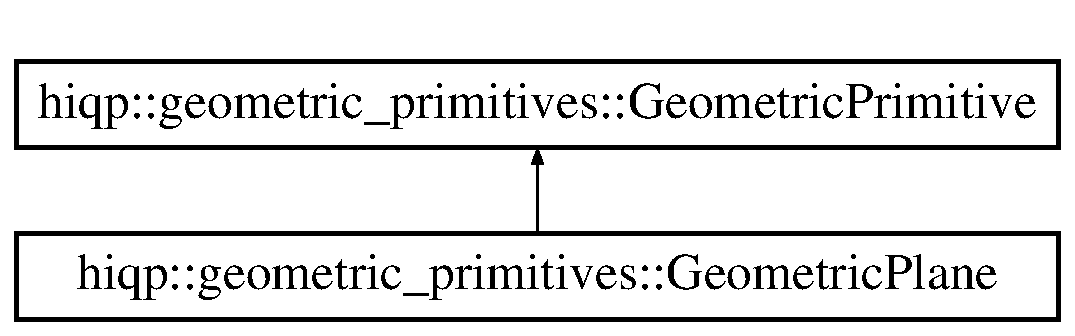
\includegraphics[height=2.000000cm]{classhiqp_1_1geometric__primitives_1_1GeometricPlane}
\end{center}
\end{figure}
\subsection*{Public Member Functions}
\begin{DoxyCompactItemize}
\item 
\hypertarget{classhiqp_1_1geometric__primitives_1_1GeometricPlane_a7d3def175b904855cf5ea41cd9af8827}{{\bfseries Geometric\-Plane} (const std\-::string \&name, const std\-::string \&frame\-\_\-id, bool visible, const std\-::vector$<$ double $>$ \&color)}\label{classhiqp_1_1geometric__primitives_1_1GeometricPlane_a7d3def175b904855cf5ea41cd9af8827}

\item 
int \hyperlink{classhiqp_1_1geometric__primitives_1_1GeometricPlane_aab4a9f1dd2c9b295e0963e53c4f13639}{init} (const std\-::vector$<$ double $>$ \&parameters)
\begin{DoxyCompactList}\small\item\em Parses a set of parameters and initializes the plane. \end{DoxyCompactList}\item 
\hypertarget{classhiqp_1_1geometric__primitives_1_1GeometricPlane_a6a5aaa0b81018b78c5fe7a1341f3004d}{const K\-D\-L\-::\-Vector \& {\bfseries get\-Normal\-K\-D\-L} ()}\label{classhiqp_1_1geometric__primitives_1_1GeometricPlane_a6a5aaa0b81018b78c5fe7a1341f3004d}

\item 
\hypertarget{classhiqp_1_1geometric__primitives_1_1GeometricPlane_aed12e48eda6560efd1987d2835a4b979}{const Eigen\-::\-Vector3d \& {\bfseries get\-Normal\-Eigen} ()}\label{classhiqp_1_1geometric__primitives_1_1GeometricPlane_aed12e48eda6560efd1987d2835a4b979}

\item 
\hypertarget{classhiqp_1_1geometric__primitives_1_1GeometricPlane_ac7944001fff45bb0f3c9a400f9242bec}{double {\bfseries get\-Offset} ()}\label{classhiqp_1_1geometric__primitives_1_1GeometricPlane_ac7944001fff45bb0f3c9a400f9242bec}

\item 
\hypertarget{classhiqp_1_1geometric__primitives_1_1GeometricPlane_a01c9232f32e246d3e35ce8e06866599d}{double {\bfseries get\-Normal\-X} ()}\label{classhiqp_1_1geometric__primitives_1_1GeometricPlane_a01c9232f32e246d3e35ce8e06866599d}

\item 
\hypertarget{classhiqp_1_1geometric__primitives_1_1GeometricPlane_ab4031f917695ab570cc46428324474a5}{double {\bfseries get\-Normal\-Y} ()}\label{classhiqp_1_1geometric__primitives_1_1GeometricPlane_ab4031f917695ab570cc46428324474a5}

\item 
\hypertarget{classhiqp_1_1geometric__primitives_1_1GeometricPlane_aa755d2dfb0603c8492ebb7efac831cfb}{double {\bfseries get\-Normal\-Z} ()}\label{classhiqp_1_1geometric__primitives_1_1GeometricPlane_aa755d2dfb0603c8492ebb7efac831cfb}

\end{DoxyCompactItemize}
\subsection*{Protected Attributes}
\begin{DoxyCompactItemize}
\item 
\hypertarget{classhiqp_1_1geometric__primitives_1_1GeometricPlane_aa9de883f574633a6d45cc00e0e23df13}{K\-D\-L\-::\-Vector {\bfseries kdl\-\_\-n\-\_\-}}\label{classhiqp_1_1geometric__primitives_1_1GeometricPlane_aa9de883f574633a6d45cc00e0e23df13}

\item 
\hypertarget{classhiqp_1_1geometric__primitives_1_1GeometricPlane_aabd33cbfa3063b0ae2b047ccce88555d}{Eigen\-::\-Vector3d {\bfseries eigen\-\_\-n\-\_\-}}\label{classhiqp_1_1geometric__primitives_1_1GeometricPlane_aabd33cbfa3063b0ae2b047ccce88555d}

\item 
\hypertarget{classhiqp_1_1geometric__primitives_1_1GeometricPlane_a72d00107f4a181f0815a06e588d0c0fd}{double {\bfseries d\-\_\-}}\label{classhiqp_1_1geometric__primitives_1_1GeometricPlane_a72d00107f4a181f0815a06e588d0c0fd}

\end{DoxyCompactItemize}


\subsection{Detailed Description}
Parameters\-: \mbox{[}n.\-x, n.\-y, n.\-z, offset\mbox{]}. 

\subsection{Member Function Documentation}
\hypertarget{classhiqp_1_1geometric__primitives_1_1GeometricPlane_aab4a9f1dd2c9b295e0963e53c4f13639}{\index{hiqp\-::geometric\-\_\-primitives\-::\-Geometric\-Plane@{hiqp\-::geometric\-\_\-primitives\-::\-Geometric\-Plane}!init@{init}}
\index{init@{init}!hiqp::geometric_primitives::GeometricPlane@{hiqp\-::geometric\-\_\-primitives\-::\-Geometric\-Plane}}
\subsubsection[{init}]{\setlength{\rightskip}{0pt plus 5cm}int hiqp\-::geometric\-\_\-primitives\-::\-Geometric\-Plane\-::init (
\begin{DoxyParamCaption}
\item[{const std\-::vector$<$ double $>$ \&}]{parameters}
\end{DoxyParamCaption}
)\hspace{0.3cm}{\ttfamily [inline]}, {\ttfamily [virtual]}}}\label{classhiqp_1_1geometric__primitives_1_1GeometricPlane_aab4a9f1dd2c9b295e0963e53c4f13639}


Parses a set of parameters and initializes the plane. 


\begin{DoxyParams}{Parameters}
{\em parameters} & should be of size 4. \par
 Indices 0-\/2 (required) defines the normal vector of the plane, \par
 index 3 (required) defines the offset of the plane in the normal direction.\\
\hline
\end{DoxyParams}
\begin{DoxyReturn}{Returns}
0 on success, -\/1 if the wrong number of parameters was sent 
\end{DoxyReturn}


Implements \hyperlink{classhiqp_1_1geometric__primitives_1_1GeometricPrimitive_a3697e5afb0121715280da649b8bd711d}{hiqp\-::geometric\-\_\-primitives\-::\-Geometric\-Primitive}.



The documentation for this class was generated from the following file\-:\begin{DoxyCompactItemize}
\item 
include/hiqp/geometric\-\_\-primitives/geometric\-\_\-plane.\-h\end{DoxyCompactItemize}

\hypertarget{classhiqp_1_1geometric__primitives_1_1GeometricPoint}{\section{hiqp\-:\-:geometric\-\_\-primitives\-:\-:Geometric\-Point Class Reference}
\label{classhiqp_1_1geometric__primitives_1_1GeometricPoint}\index{hiqp\-::geometric\-\_\-primitives\-::\-Geometric\-Point@{hiqp\-::geometric\-\_\-primitives\-::\-Geometric\-Point}}
}


Parameters\-: \mbox{[}x, y, z\mbox{]}.  




{\ttfamily \#include $<$geometric\-\_\-point.\-h$>$}

Inheritance diagram for hiqp\-:\-:geometric\-\_\-primitives\-:\-:Geometric\-Point\-:\begin{figure}[H]
\begin{center}
\leavevmode
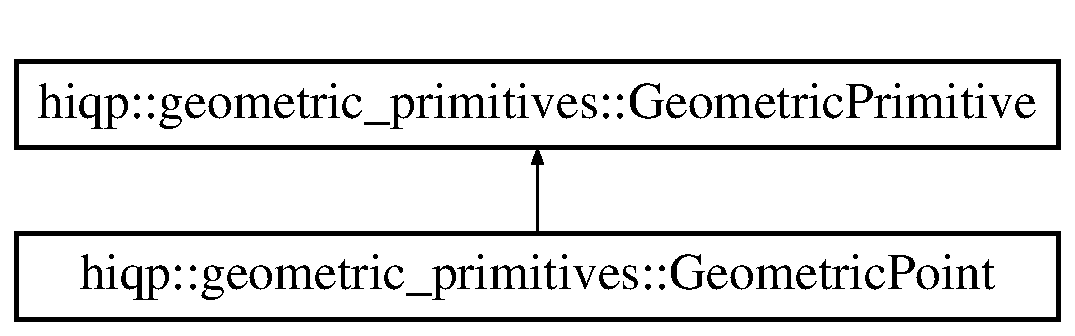
\includegraphics[height=2.000000cm]{classhiqp_1_1geometric__primitives_1_1GeometricPoint}
\end{center}
\end{figure}
\subsection*{Public Member Functions}
\begin{DoxyCompactItemize}
\item 
\hypertarget{classhiqp_1_1geometric__primitives_1_1GeometricPoint_a4e3dd5ac625cac7ccf795b6b2f1facfd}{{\bfseries Geometric\-Point} (const std\-::string \&name, const std\-::string \&frame\-\_\-id, bool visible, const std\-::vector$<$ double $>$ \&color)}\label{classhiqp_1_1geometric__primitives_1_1GeometricPoint_a4e3dd5ac625cac7ccf795b6b2f1facfd}

\item 
int \hyperlink{classhiqp_1_1geometric__primitives_1_1GeometricPoint_a2e055a55316c83c22a26ba85e9da975d}{init} (const std\-::vector$<$ double $>$ \&parameters)
\begin{DoxyCompactList}\small\item\em Parses a set of parameters and initializes the point. \end{DoxyCompactList}\item 
\hypertarget{classhiqp_1_1geometric__primitives_1_1GeometricPoint_a5515141a01be0bc90421a530cc72fe32}{const K\-D\-L\-::\-Vector \& {\bfseries get\-Point\-K\-D\-L} ()}\label{classhiqp_1_1geometric__primitives_1_1GeometricPoint_a5515141a01be0bc90421a530cc72fe32}

\item 
\hypertarget{classhiqp_1_1geometric__primitives_1_1GeometricPoint_a56500d7851c6488ece9fe62c57ee4ea0}{const Eigen\-::\-Vector3d \& {\bfseries get\-Point\-Eigen} ()}\label{classhiqp_1_1geometric__primitives_1_1GeometricPoint_a56500d7851c6488ece9fe62c57ee4ea0}

\item 
\hypertarget{classhiqp_1_1geometric__primitives_1_1GeometricPoint_a573b66ccd7b4a2071ddce07f479ebfb5}{double {\bfseries get\-X} ()}\label{classhiqp_1_1geometric__primitives_1_1GeometricPoint_a573b66ccd7b4a2071ddce07f479ebfb5}

\item 
\hypertarget{classhiqp_1_1geometric__primitives_1_1GeometricPoint_a40fb3e3735c431b798b836c68dd82e89}{double {\bfseries get\-Y} ()}\label{classhiqp_1_1geometric__primitives_1_1GeometricPoint_a40fb3e3735c431b798b836c68dd82e89}

\item 
\hypertarget{classhiqp_1_1geometric__primitives_1_1GeometricPoint_a4786d47f1c74466c1a703a53379cddd9}{double {\bfseries get\-Z} ()}\label{classhiqp_1_1geometric__primitives_1_1GeometricPoint_a4786d47f1c74466c1a703a53379cddd9}

\end{DoxyCompactItemize}
\subsection*{Protected Attributes}
\begin{DoxyCompactItemize}
\item 
\hypertarget{classhiqp_1_1geometric__primitives_1_1GeometricPoint_a4433663af43188e0f349fa0bebfb0078}{K\-D\-L\-::\-Vector {\bfseries kdl\-\_\-p\-\_\-}}\label{classhiqp_1_1geometric__primitives_1_1GeometricPoint_a4433663af43188e0f349fa0bebfb0078}

\item 
\hypertarget{classhiqp_1_1geometric__primitives_1_1GeometricPoint_ad19898465cb7f9621030edc32edf4364}{Eigen\-::\-Vector3d {\bfseries eigen\-\_\-p\-\_\-}}\label{classhiqp_1_1geometric__primitives_1_1GeometricPoint_ad19898465cb7f9621030edc32edf4364}

\end{DoxyCompactItemize}


\subsection{Detailed Description}
Parameters\-: \mbox{[}x, y, z\mbox{]}. 

\subsection{Member Function Documentation}
\hypertarget{classhiqp_1_1geometric__primitives_1_1GeometricPoint_a2e055a55316c83c22a26ba85e9da975d}{\index{hiqp\-::geometric\-\_\-primitives\-::\-Geometric\-Point@{hiqp\-::geometric\-\_\-primitives\-::\-Geometric\-Point}!init@{init}}
\index{init@{init}!hiqp::geometric_primitives::GeometricPoint@{hiqp\-::geometric\-\_\-primitives\-::\-Geometric\-Point}}
\subsubsection[{init}]{\setlength{\rightskip}{0pt plus 5cm}int hiqp\-::geometric\-\_\-primitives\-::\-Geometric\-Point\-::init (
\begin{DoxyParamCaption}
\item[{const std\-::vector$<$ double $>$ \&}]{parameters}
\end{DoxyParamCaption}
)\hspace{0.3cm}{\ttfamily [inline]}, {\ttfamily [virtual]}}}\label{classhiqp_1_1geometric__primitives_1_1GeometricPoint_a2e055a55316c83c22a26ba85e9da975d}


Parses a set of parameters and initializes the point. 


\begin{DoxyParams}{Parameters}
{\em parameters} & should be of size 3. \par
 Indices 0-\/2 (required) defines the position of the point.\\
\hline
\end{DoxyParams}
\begin{DoxyReturn}{Returns}
0 on success, -\/1 if the wrong number of parameters was sent 
\end{DoxyReturn}


Implements \hyperlink{classhiqp_1_1geometric__primitives_1_1GeometricPrimitive_a3697e5afb0121715280da649b8bd711d}{hiqp\-::geometric\-\_\-primitives\-::\-Geometric\-Primitive}.



The documentation for this class was generated from the following file\-:\begin{DoxyCompactItemize}
\item 
include/hiqp/geometric\-\_\-primitives/geometric\-\_\-point.\-h\end{DoxyCompactItemize}

\hypertarget{classhiqp_1_1geometric__primitives_1_1GeometricPrimitive}{\section{hiqp\-:\-:geometric\-\_\-primitives\-:\-:Geometric\-Primitive Class Reference}
\label{classhiqp_1_1geometric__primitives_1_1GeometricPrimitive}\index{hiqp\-::geometric\-\_\-primitives\-::\-Geometric\-Primitive@{hiqp\-::geometric\-\_\-primitives\-::\-Geometric\-Primitive}}
}


Abstract base class for all geometric primitives.  




{\ttfamily \#include $<$geometric\-\_\-primitive.\-h$>$}

Inheritance diagram for hiqp\-:\-:geometric\-\_\-primitives\-:\-:Geometric\-Primitive\-:\begin{figure}[H]
\begin{center}
\leavevmode
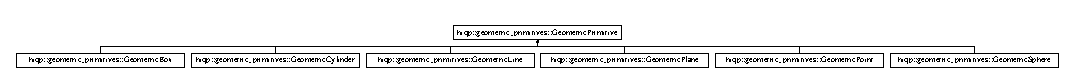
\includegraphics[height=0.678788cm]{classhiqp_1_1geometric__primitives_1_1GeometricPrimitive}
\end{center}
\end{figure}
\subsection*{Public Member Functions}
\begin{DoxyCompactItemize}
\item 
\hypertarget{classhiqp_1_1geometric__primitives_1_1GeometricPrimitive_a4dfa06c8f664ce1206d09ecd7b6d4b22}{{\bfseries Geometric\-Primitive} (const std\-::string \&name, const std\-::string \&frame\-\_\-id, bool visible, const std\-::vector$<$ double $>$ \&color)}\label{classhiqp_1_1geometric__primitives_1_1GeometricPrimitive_a4dfa06c8f664ce1206d09ecd7b6d4b22}

\item 
\hypertarget{classhiqp_1_1geometric__primitives_1_1GeometricPrimitive_a3697e5afb0121715280da649b8bd711d}{virtual int \hyperlink{classhiqp_1_1geometric__primitives_1_1GeometricPrimitive_a3697e5afb0121715280da649b8bd711d}{init} (const std\-::vector$<$ double $>$ \&parameters)=0}\label{classhiqp_1_1geometric__primitives_1_1GeometricPrimitive_a3697e5afb0121715280da649b8bd711d}

\begin{DoxyCompactList}\small\item\em Needs to be specified by the inheriting class. \end{DoxyCompactList}\item 
\hypertarget{classhiqp_1_1geometric__primitives_1_1GeometricPrimitive_adb67fd231dcc0d5b544ece9f0fa1bdf5}{void {\bfseries set\-Id} (unsigned int id)}\label{classhiqp_1_1geometric__primitives_1_1GeometricPrimitive_adb67fd231dcc0d5b544ece9f0fa1bdf5}

\item 
\hypertarget{classhiqp_1_1geometric__primitives_1_1GeometricPrimitive_a7c07e7e6d768a5b92b6b08950aac9df6}{unsigned int {\bfseries get\-Id} ()}\label{classhiqp_1_1geometric__primitives_1_1GeometricPrimitive_a7c07e7e6d768a5b92b6b08950aac9df6}

\item 
\hypertarget{classhiqp_1_1geometric__primitives_1_1GeometricPrimitive_a9e3448f020001187585f48f164ae54ea}{std\-::string {\bfseries get\-Name} ()}\label{classhiqp_1_1geometric__primitives_1_1GeometricPrimitive_a9e3448f020001187585f48f164ae54ea}

\item 
\hypertarget{classhiqp_1_1geometric__primitives_1_1GeometricPrimitive_a358c7a2b87edc3142e1975047e3fbdad}{std\-::string {\bfseries get\-Frame\-Id} ()}\label{classhiqp_1_1geometric__primitives_1_1GeometricPrimitive_a358c7a2b87edc3142e1975047e3fbdad}

\item 
\hypertarget{classhiqp_1_1geometric__primitives_1_1GeometricPrimitive_a4a35b6e42bec938524c7e1f92bcaecf5}{bool {\bfseries is\-Visible} ()}\label{classhiqp_1_1geometric__primitives_1_1GeometricPrimitive_a4a35b6e42bec938524c7e1f92bcaecf5}

\item 
\hypertarget{classhiqp_1_1geometric__primitives_1_1GeometricPrimitive_af20c0505a037569959928ee874a78ada}{double {\bfseries get\-Red\-Component} ()}\label{classhiqp_1_1geometric__primitives_1_1GeometricPrimitive_af20c0505a037569959928ee874a78ada}

\item 
\hypertarget{classhiqp_1_1geometric__primitives_1_1GeometricPrimitive_a09d0c7301194102618252625b69c0a8a}{double {\bfseries get\-Green\-Component} ()}\label{classhiqp_1_1geometric__primitives_1_1GeometricPrimitive_a09d0c7301194102618252625b69c0a8a}

\item 
\hypertarget{classhiqp_1_1geometric__primitives_1_1GeometricPrimitive_afc88cc98a589c1e3be660be16cff6071}{double {\bfseries get\-Blue\-Component} ()}\label{classhiqp_1_1geometric__primitives_1_1GeometricPrimitive_afc88cc98a589c1e3be660be16cff6071}

\item 
\hypertarget{classhiqp_1_1geometric__primitives_1_1GeometricPrimitive_a7d9a08ec7a9212c8f73e3d653651b309}{double {\bfseries get\-Alpha\-Component} ()}\label{classhiqp_1_1geometric__primitives_1_1GeometricPrimitive_a7d9a08ec7a9212c8f73e3d653651b309}

\end{DoxyCompactItemize}
\subsection*{Protected Attributes}
\begin{DoxyCompactItemize}
\item 
\hypertarget{classhiqp_1_1geometric__primitives_1_1GeometricPrimitive_a3c0b86477197e83a007864ab4bddf64d}{std\-::string {\bfseries name\-\_\-}}\label{classhiqp_1_1geometric__primitives_1_1GeometricPrimitive_a3c0b86477197e83a007864ab4bddf64d}

\item 
\hypertarget{classhiqp_1_1geometric__primitives_1_1GeometricPrimitive_adf47c6318853048d687374d6f75be69b}{std\-::string {\bfseries frame\-\_\-id\-\_\-}}\label{classhiqp_1_1geometric__primitives_1_1GeometricPrimitive_adf47c6318853048d687374d6f75be69b}

\item 
\hypertarget{classhiqp_1_1geometric__primitives_1_1GeometricPrimitive_a0f59fa89007d192bde05ca65df75a592}{bool {\bfseries visible\-\_\-}}\label{classhiqp_1_1geometric__primitives_1_1GeometricPrimitive_a0f59fa89007d192bde05ca65df75a592}

\item 
\hypertarget{classhiqp_1_1geometric__primitives_1_1GeometricPrimitive_a4ad5dff2d31d3a5dc407f5fb5d8188b8}{unsigned int {\bfseries id\-\_\-}}\label{classhiqp_1_1geometric__primitives_1_1GeometricPrimitive_a4ad5dff2d31d3a5dc407f5fb5d8188b8}

\item 
\hypertarget{classhiqp_1_1geometric__primitives_1_1GeometricPrimitive_a8459802c1669f64bf61189b89bd5c68d}{double {\bfseries r\-\_\-}}\label{classhiqp_1_1geometric__primitives_1_1GeometricPrimitive_a8459802c1669f64bf61189b89bd5c68d}

\item 
\hypertarget{classhiqp_1_1geometric__primitives_1_1GeometricPrimitive_a94108ca48b0d01d2d3df483561a802b3}{double {\bfseries g\-\_\-}}\label{classhiqp_1_1geometric__primitives_1_1GeometricPrimitive_a94108ca48b0d01d2d3df483561a802b3}

\item 
\hypertarget{classhiqp_1_1geometric__primitives_1_1GeometricPrimitive_ae74366f413fb40af4f8a48b297a1a79c}{double {\bfseries b\-\_\-}}\label{classhiqp_1_1geometric__primitives_1_1GeometricPrimitive_ae74366f413fb40af4f8a48b297a1a79c}

\item 
\hypertarget{classhiqp_1_1geometric__primitives_1_1GeometricPrimitive_af4bf3cef98a1257ba054234fd6acd5d4}{double {\bfseries a\-\_\-}}\label{classhiqp_1_1geometric__primitives_1_1GeometricPrimitive_af4bf3cef98a1257ba054234fd6acd5d4}

\end{DoxyCompactItemize}


\subsection{Detailed Description}
Abstract base class for all geometric primitives. 

The documentation for this class was generated from the following file\-:\begin{DoxyCompactItemize}
\item 
include/hiqp/geometric\-\_\-primitives/geometric\-\_\-primitive.\-h\end{DoxyCompactItemize}

\hypertarget{classhiqp_1_1geometric__primitives_1_1GeometricPrimitiveMap}{\section{hiqp\-:\-:geometric\-\_\-primitives\-:\-:Geometric\-Primitive\-Map Class Reference}
\label{classhiqp_1_1geometric__primitives_1_1GeometricPrimitiveMap}\index{hiqp\-::geometric\-\_\-primitives\-::\-Geometric\-Primitive\-Map@{hiqp\-::geometric\-\_\-primitives\-::\-Geometric\-Primitive\-Map}}
}


A common map data structure for all geometric primitive types.  




{\ttfamily \#include $<$geometric\-\_\-primitive\-\_\-map.\-h$>$}

\subsection*{Public Member Functions}
\begin{DoxyCompactItemize}
\item 
\hypertarget{classhiqp_1_1geometric__primitives_1_1GeometricPrimitiveMap_ae59d213ebfa9f3d22678e048928cf565}{{\bfseries Geometric\-Primitive\-Map} (\hyperlink{classhiqp_1_1Visualizer}{Visualizer} $\ast$visualizer)}\label{classhiqp_1_1geometric__primitives_1_1GeometricPrimitiveMap_ae59d213ebfa9f3d22678e048928cf565}

\item 
\hypertarget{classhiqp_1_1geometric__primitives_1_1GeometricPrimitiveMap_a6ddc5d3b4e8e44748fbb0c9e66957952}{int {\bfseries add\-Geometric\-Primitive} (const std\-::string \&name, const std\-::string \&type, const std\-::string \&frame\-\_\-id, bool visible, const std\-::vector$<$ double $>$ \&color, const std\-::vector$<$ double $>$ \&parameters)}\label{classhiqp_1_1geometric__primitives_1_1GeometricPrimitiveMap_a6ddc5d3b4e8e44748fbb0c9e66957952}

\item 
int \hyperlink{classhiqp_1_1geometric__primitives_1_1GeometricPrimitiveMap_a07d04c1a3bb164bb501bd03cc6bc1eae}{remove\-Geometric\-Primitive} (std\-::string name)
\item 
int \hyperlink{classhiqp_1_1geometric__primitives_1_1GeometricPrimitiveMap_aed92b78b51ccd075d226b003f9576476}{clear} ()
\item 
\hypertarget{classhiqp_1_1geometric__primitives_1_1GeometricPrimitiveMap_a51ccc8c0ff1434c8b8d1bcc2d0d9bbbf}{{\footnotesize template$<$typename Primitive\-Type $>$ }\\Primitive\-Type $\ast$ {\bfseries get\-Geometric\-Primitive} (const std\-::string \&name)}\label{classhiqp_1_1geometric__primitives_1_1GeometricPrimitiveMap_a51ccc8c0ff1434c8b8d1bcc2d0d9bbbf}

\item 
\hypertarget{classhiqp_1_1geometric__primitives_1_1GeometricPrimitiveMap_a844d0776ad4465b25825d91d2eb1f38a}{{\footnotesize template$<$typename Primitive\-Type $>$ }\\void {\bfseries update\-Geometric\-Primitive} (const std\-::string \&name, const std\-::vector$<$ double $>$ \&parameters)}\label{classhiqp_1_1geometric__primitives_1_1GeometricPrimitiveMap_a844d0776ad4465b25825d91d2eb1f38a}

\item 
\hypertarget{classhiqp_1_1geometric__primitives_1_1GeometricPrimitiveMap_a401b6481e8e08e26466dbd06c8b62ee5}{void {\bfseries redraw\-All\-Primitives} ()}\label{classhiqp_1_1geometric__primitives_1_1GeometricPrimitiveMap_a401b6481e8e08e26466dbd06c8b62ee5}

\item 
\hypertarget{classhiqp_1_1geometric__primitives_1_1GeometricPrimitiveMap_a493d855058eaf3c15e694a1641abb102}{void {\bfseries add\-Dependency\-To\-Primitive} (const std\-::string \&name, const std\-::string \&id)}\label{classhiqp_1_1geometric__primitives_1_1GeometricPrimitiveMap_a493d855058eaf3c15e694a1641abb102}

\item 
\hypertarget{classhiqp_1_1geometric__primitives_1_1GeometricPrimitiveMap_abab3cf9f15237f9de30a488962b63bf3}{void {\bfseries remove\-Dependency} (const std\-::string \&id)}\label{classhiqp_1_1geometric__primitives_1_1GeometricPrimitiveMap_abab3cf9f15237f9de30a488962b63bf3}

\item 
\hypertarget{classhiqp_1_1geometric__primitives_1_1GeometricPrimitiveMap_a19db1c3b7ebdd46dcf50f5505b60a6bc}{{\footnotesize template$<$$>$ }\\\hyperlink{classhiqp_1_1geometric__primitives_1_1GeometricPoint}{Geometric\-Point} $\ast$ {\bfseries get\-Geometric\-Primitive} (const std\-::string \&name)}\label{classhiqp_1_1geometric__primitives_1_1GeometricPrimitiveMap_a19db1c3b7ebdd46dcf50f5505b60a6bc}

\item 
\hypertarget{classhiqp_1_1geometric__primitives_1_1GeometricPrimitiveMap_ade38cde2dd29b532832c48b47f3f10a8}{{\footnotesize template$<$$>$ }\\\hyperlink{classhiqp_1_1geometric__primitives_1_1GeometricLine}{Geometric\-Line} $\ast$ {\bfseries get\-Geometric\-Primitive} (const std\-::string \&name)}\label{classhiqp_1_1geometric__primitives_1_1GeometricPrimitiveMap_ade38cde2dd29b532832c48b47f3f10a8}

\item 
\hypertarget{classhiqp_1_1geometric__primitives_1_1GeometricPrimitiveMap_a7dc61cfb44db9bba0cdce8729c9269a0}{{\footnotesize template$<$$>$ }\\\hyperlink{classhiqp_1_1geometric__primitives_1_1GeometricPlane}{Geometric\-Plane} $\ast$ {\bfseries get\-Geometric\-Primitive} (const std\-::string \&name)}\label{classhiqp_1_1geometric__primitives_1_1GeometricPrimitiveMap_a7dc61cfb44db9bba0cdce8729c9269a0}

\item 
\hypertarget{classhiqp_1_1geometric__primitives_1_1GeometricPrimitiveMap_a75164f9183ed4e0979cd17300889067f}{{\footnotesize template$<$$>$ }\\\hyperlink{classhiqp_1_1geometric__primitives_1_1GeometricBox}{Geometric\-Box} $\ast$ {\bfseries get\-Geometric\-Primitive} (const std\-::string \&name)}\label{classhiqp_1_1geometric__primitives_1_1GeometricPrimitiveMap_a75164f9183ed4e0979cd17300889067f}

\item 
\hypertarget{classhiqp_1_1geometric__primitives_1_1GeometricPrimitiveMap_ae728aa00516f80aaf850359a548b6473}{{\footnotesize template$<$$>$ }\\\hyperlink{classhiqp_1_1geometric__primitives_1_1GeometricCylinder}{Geometric\-Cylinder} $\ast$ {\bfseries get\-Geometric\-Primitive} (const std\-::string \&name)}\label{classhiqp_1_1geometric__primitives_1_1GeometricPrimitiveMap_ae728aa00516f80aaf850359a548b6473}

\item 
\hypertarget{classhiqp_1_1geometric__primitives_1_1GeometricPrimitiveMap_a71bba5bd417ee2a5ae8179aabc10cf79}{{\footnotesize template$<$$>$ }\\\hyperlink{classhiqp_1_1geometric__primitives_1_1GeometricSphere}{Geometric\-Sphere} $\ast$ {\bfseries get\-Geometric\-Primitive} (const std\-::string \&name)}\label{classhiqp_1_1geometric__primitives_1_1GeometricPrimitiveMap_a71bba5bd417ee2a5ae8179aabc10cf79}

\item 
\hypertarget{classhiqp_1_1geometric__primitives_1_1GeometricPrimitiveMap_afede16f63460bb07795ee12b426ee919}{{\footnotesize template$<$$>$ }\\void {\bfseries update\-Geometric\-Primitive} (const std\-::string \&name, const std\-::vector$<$ double $>$ \&parameters)}\label{classhiqp_1_1geometric__primitives_1_1GeometricPrimitiveMap_afede16f63460bb07795ee12b426ee919}

\item 
\hypertarget{classhiqp_1_1geometric__primitives_1_1GeometricPrimitiveMap_afede16f63460bb07795ee12b426ee919}{{\footnotesize template$<$$>$ }\\void {\bfseries update\-Geometric\-Primitive} (const std\-::string \&name, const std\-::vector$<$ double $>$ \&parameters)}\label{classhiqp_1_1geometric__primitives_1_1GeometricPrimitiveMap_afede16f63460bb07795ee12b426ee919}

\item 
\hypertarget{classhiqp_1_1geometric__primitives_1_1GeometricPrimitiveMap_afede16f63460bb07795ee12b426ee919}{{\footnotesize template$<$$>$ }\\void {\bfseries update\-Geometric\-Primitive} (const std\-::string \&name, const std\-::vector$<$ double $>$ \&parameters)}\label{classhiqp_1_1geometric__primitives_1_1GeometricPrimitiveMap_afede16f63460bb07795ee12b426ee919}

\item 
\hypertarget{classhiqp_1_1geometric__primitives_1_1GeometricPrimitiveMap_afede16f63460bb07795ee12b426ee919}{{\footnotesize template$<$$>$ }\\void {\bfseries update\-Geometric\-Primitive} (const std\-::string \&name, const std\-::vector$<$ double $>$ \&parameters)}\label{classhiqp_1_1geometric__primitives_1_1GeometricPrimitiveMap_afede16f63460bb07795ee12b426ee919}

\item 
\hypertarget{classhiqp_1_1geometric__primitives_1_1GeometricPrimitiveMap_afede16f63460bb07795ee12b426ee919}{{\footnotesize template$<$$>$ }\\void {\bfseries update\-Geometric\-Primitive} (const std\-::string \&name, const std\-::vector$<$ double $>$ \&parameters)}\label{classhiqp_1_1geometric__primitives_1_1GeometricPrimitiveMap_afede16f63460bb07795ee12b426ee919}

\item 
\hypertarget{classhiqp_1_1geometric__primitives_1_1GeometricPrimitiveMap_afede16f63460bb07795ee12b426ee919}{{\footnotesize template$<$$>$ }\\void {\bfseries update\-Geometric\-Primitive} (const std\-::string \&name, const std\-::vector$<$ double $>$ \&parameters)}\label{classhiqp_1_1geometric__primitives_1_1GeometricPrimitiveMap_afede16f63460bb07795ee12b426ee919}

\end{DoxyCompactItemize}


\subsection{Detailed Description}
A common map data structure for all geometric primitive types. 

\subsection{Member Function Documentation}
\hypertarget{classhiqp_1_1geometric__primitives_1_1GeometricPrimitiveMap_aed92b78b51ccd075d226b003f9576476}{\index{hiqp\-::geometric\-\_\-primitives\-::\-Geometric\-Primitive\-Map@{hiqp\-::geometric\-\_\-primitives\-::\-Geometric\-Primitive\-Map}!clear@{clear}}
\index{clear@{clear}!hiqp::geometric_primitives::GeometricPrimitiveMap@{hiqp\-::geometric\-\_\-primitives\-::\-Geometric\-Primitive\-Map}}
\subsubsection[{clear}]{\setlength{\rightskip}{0pt plus 5cm}int hiqp\-::geometric\-\_\-primitives\-::\-Geometric\-Primitive\-Map\-::clear (
\begin{DoxyParamCaption}
{}
\end{DoxyParamCaption}
)}}\label{classhiqp_1_1geometric__primitives_1_1GeometricPrimitiveMap_aed92b78b51ccd075d226b003f9576476}
\begin{DoxyRefDesc}{Todo}
\item[\hyperlink{todo__todo000002}{Todo}]primitives with dependencies to tasks shall not be deleted! \end{DoxyRefDesc}
\hypertarget{classhiqp_1_1geometric__primitives_1_1GeometricPrimitiveMap_a07d04c1a3bb164bb501bd03cc6bc1eae}{\index{hiqp\-::geometric\-\_\-primitives\-::\-Geometric\-Primitive\-Map@{hiqp\-::geometric\-\_\-primitives\-::\-Geometric\-Primitive\-Map}!remove\-Geometric\-Primitive@{remove\-Geometric\-Primitive}}
\index{remove\-Geometric\-Primitive@{remove\-Geometric\-Primitive}!hiqp::geometric_primitives::GeometricPrimitiveMap@{hiqp\-::geometric\-\_\-primitives\-::\-Geometric\-Primitive\-Map}}
\subsubsection[{remove\-Geometric\-Primitive}]{\setlength{\rightskip}{0pt plus 5cm}int hiqp\-::geometric\-\_\-primitives\-::\-Geometric\-Primitive\-Map\-::remove\-Geometric\-Primitive (
\begin{DoxyParamCaption}
\item[{std\-::string}]{name}
\end{DoxyParamCaption}
)}}\label{classhiqp_1_1geometric__primitives_1_1GeometricPrimitiveMap_a07d04c1a3bb164bb501bd03cc6bc1eae}
\begin{DoxyRefDesc}{Todo}
\item[\hyperlink{todo__todo000001}{Todo}]primitives should have dependencies on tasks and not be removable if dependencies exists! \end{DoxyRefDesc}


The documentation for this class was generated from the following files\-:\begin{DoxyCompactItemize}
\item 
include/hiqp/geometric\-\_\-primitives/geometric\-\_\-primitive\-\_\-map.\-h\item 
src/geometric\-\_\-primitives/\hyperlink{geometric__primitive__map_8cpp}{geometric\-\_\-primitive\-\_\-map.\-cpp}\end{DoxyCompactItemize}

\hypertarget{classhiqp_1_1geometric__primitives_1_1GeometricSphere}{\section{hiqp\-:\-:geometric\-\_\-primitives\-:\-:Geometric\-Sphere Class Reference}
\label{classhiqp_1_1geometric__primitives_1_1GeometricSphere}\index{hiqp\-::geometric\-\_\-primitives\-::\-Geometric\-Sphere@{hiqp\-::geometric\-\_\-primitives\-::\-Geometric\-Sphere}}
}


Parameters\-: \mbox{[}x, y, z, radius\mbox{]}.  




{\ttfamily \#include $<$geometric\-\_\-sphere.\-h$>$}

Inheritance diagram for hiqp\-:\-:geometric\-\_\-primitives\-:\-:Geometric\-Sphere\-:\begin{figure}[H]
\begin{center}
\leavevmode
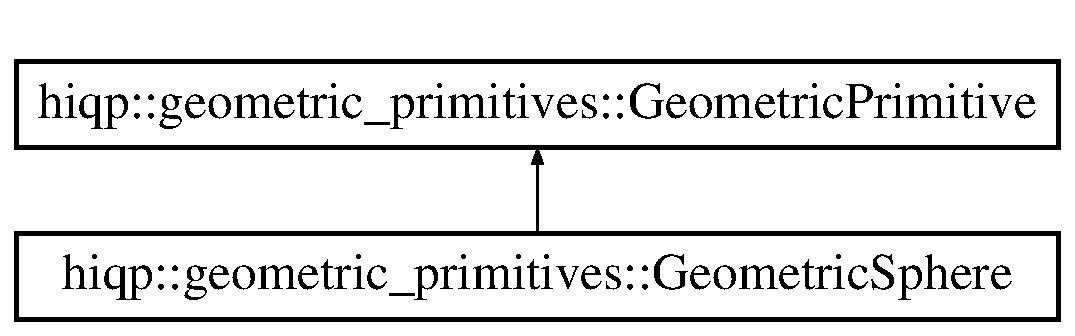
\includegraphics[height=2.000000cm]{classhiqp_1_1geometric__primitives_1_1GeometricSphere}
\end{center}
\end{figure}
\subsection*{Public Member Functions}
\begin{DoxyCompactItemize}
\item 
\hypertarget{classhiqp_1_1geometric__primitives_1_1GeometricSphere_a79a504eeb43a92782b9977dfaabc46de}{{\bfseries Geometric\-Sphere} (const std\-::string \&name, const std\-::string \&frame\-\_\-id, bool visible, const std\-::vector$<$ double $>$ \&color)}\label{classhiqp_1_1geometric__primitives_1_1GeometricSphere_a79a504eeb43a92782b9977dfaabc46de}

\item 
int \hyperlink{classhiqp_1_1geometric__primitives_1_1GeometricSphere_aa291157616f08f80ded39aa29cd3589a}{init} (const std\-::vector$<$ double $>$ \&parameters)
\begin{DoxyCompactList}\small\item\em Parses a set of parameters and initializes the sphere. \end{DoxyCompactList}\item 
\hypertarget{classhiqp_1_1geometric__primitives_1_1GeometricSphere_ab56e9bf7f22278e100f740e4ff95dc6d}{const K\-D\-L\-::\-Vector \& {\bfseries get\-Center\-K\-D\-L} ()}\label{classhiqp_1_1geometric__primitives_1_1GeometricSphere_ab56e9bf7f22278e100f740e4ff95dc6d}

\item 
\hypertarget{classhiqp_1_1geometric__primitives_1_1GeometricSphere_a7003d1beed56d74545ad701bb8c267e2}{const Eigen\-::\-Vector3d \& {\bfseries get\-Center\-Eigen} ()}\label{classhiqp_1_1geometric__primitives_1_1GeometricSphere_a7003d1beed56d74545ad701bb8c267e2}

\item 
\hypertarget{classhiqp_1_1geometric__primitives_1_1GeometricSphere_a2ed658030d5679dfb61546b081719170}{double {\bfseries get\-Radius} ()}\label{classhiqp_1_1geometric__primitives_1_1GeometricSphere_a2ed658030d5679dfb61546b081719170}

\item 
\hypertarget{classhiqp_1_1geometric__primitives_1_1GeometricSphere_a0a861789beade3d8b897448cb3ed8bd9}{double {\bfseries get\-X} ()}\label{classhiqp_1_1geometric__primitives_1_1GeometricSphere_a0a861789beade3d8b897448cb3ed8bd9}

\item 
\hypertarget{classhiqp_1_1geometric__primitives_1_1GeometricSphere_a773735994c0f1f0341e71669f146118d}{double {\bfseries get\-Y} ()}\label{classhiqp_1_1geometric__primitives_1_1GeometricSphere_a773735994c0f1f0341e71669f146118d}

\item 
\hypertarget{classhiqp_1_1geometric__primitives_1_1GeometricSphere_a2340c72ca73f5a424fd831c084430ba6}{double {\bfseries get\-Z} ()}\label{classhiqp_1_1geometric__primitives_1_1GeometricSphere_a2340c72ca73f5a424fd831c084430ba6}

\end{DoxyCompactItemize}
\subsection*{Protected Attributes}
\begin{DoxyCompactItemize}
\item 
\hypertarget{classhiqp_1_1geometric__primitives_1_1GeometricSphere_ad1d0e7dbde85c588ef7254765246db42}{K\-D\-L\-::\-Vector {\bfseries kdl\-\_\-p\-\_\-}}\label{classhiqp_1_1geometric__primitives_1_1GeometricSphere_ad1d0e7dbde85c588ef7254765246db42}

\item 
\hypertarget{classhiqp_1_1geometric__primitives_1_1GeometricSphere_a73d583004d75108eb963de03fccfb3a0}{Eigen\-::\-Vector3d {\bfseries eigen\-\_\-p\-\_\-}}\label{classhiqp_1_1geometric__primitives_1_1GeometricSphere_a73d583004d75108eb963de03fccfb3a0}

\item 
\hypertarget{classhiqp_1_1geometric__primitives_1_1GeometricSphere_a6d806a0619054ac2989490056c98e7f7}{double {\bfseries radius\-\_\-}}\label{classhiqp_1_1geometric__primitives_1_1GeometricSphere_a6d806a0619054ac2989490056c98e7f7}

\end{DoxyCompactItemize}


\subsection{Detailed Description}
Parameters\-: \mbox{[}x, y, z, radius\mbox{]}. 

\subsection{Member Function Documentation}
\hypertarget{classhiqp_1_1geometric__primitives_1_1GeometricSphere_aa291157616f08f80ded39aa29cd3589a}{\index{hiqp\-::geometric\-\_\-primitives\-::\-Geometric\-Sphere@{hiqp\-::geometric\-\_\-primitives\-::\-Geometric\-Sphere}!init@{init}}
\index{init@{init}!hiqp::geometric_primitives::GeometricSphere@{hiqp\-::geometric\-\_\-primitives\-::\-Geometric\-Sphere}}
\subsubsection[{init}]{\setlength{\rightskip}{0pt plus 5cm}int hiqp\-::geometric\-\_\-primitives\-::\-Geometric\-Sphere\-::init (
\begin{DoxyParamCaption}
\item[{const std\-::vector$<$ double $>$ \&}]{parameters}
\end{DoxyParamCaption}
)\hspace{0.3cm}{\ttfamily [inline]}, {\ttfamily [virtual]}}}\label{classhiqp_1_1geometric__primitives_1_1GeometricSphere_aa291157616f08f80ded39aa29cd3589a}


Parses a set of parameters and initializes the sphere. 


\begin{DoxyParams}{Parameters}
{\em parameters} & should be of size 4. \par
 Indices 0-\/2 (required) defines the position of the center of the sphere, \par
 index 3 (required) defines the radius of the sphere.\\
\hline
\end{DoxyParams}
\begin{DoxyReturn}{Returns}
0 on success, -\/1 if the wrong number of parameters was sent 
\end{DoxyReturn}


Implements \hyperlink{classhiqp_1_1geometric__primitives_1_1GeometricPrimitive_a3697e5afb0121715280da649b8bd711d}{hiqp\-::geometric\-\_\-primitives\-::\-Geometric\-Primitive}.



The documentation for this class was generated from the following file\-:\begin{DoxyCompactItemize}
\item 
include/hiqp/geometric\-\_\-primitives/geometric\-\_\-sphere.\-h\end{DoxyCompactItemize}

\hypertarget{classhiqp_1_1HiQPSolver}{\section{hiqp\-:\-:Hi\-Q\-P\-Solver Class Reference}
\label{classhiqp_1_1HiQPSolver}\index{hiqp\-::\-Hi\-Q\-P\-Solver@{hiqp\-::\-Hi\-Q\-P\-Solver}}
}
Inheritance diagram for hiqp\-:\-:Hi\-Q\-P\-Solver\-:\begin{figure}[H]
\begin{center}
\leavevmode
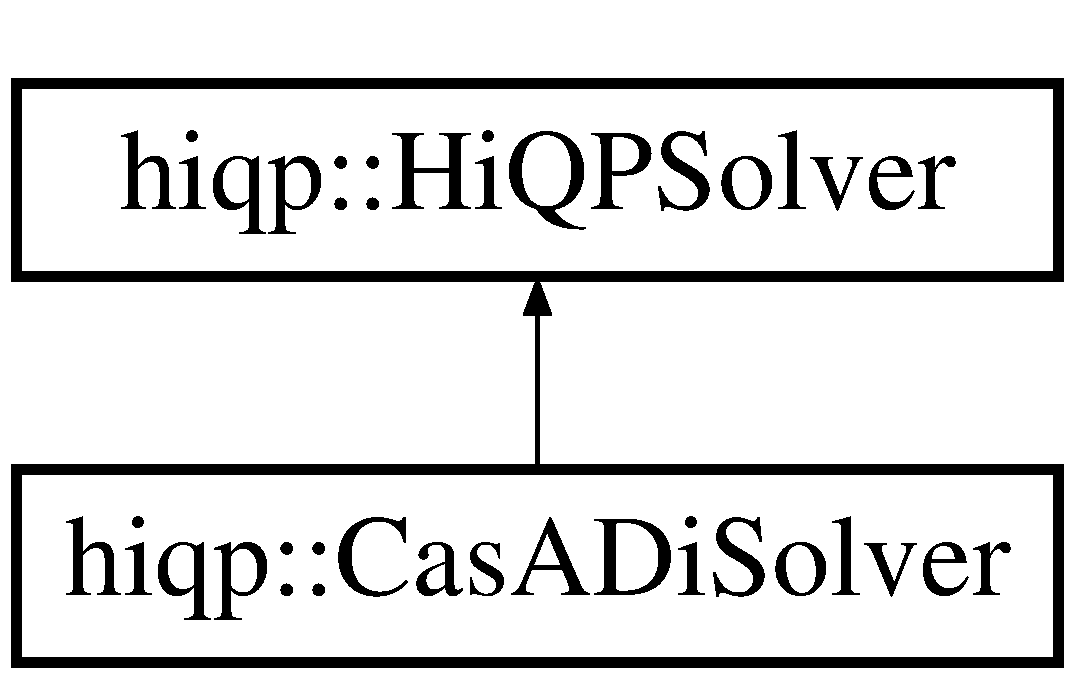
\includegraphics[height=2.000000cm]{classhiqp_1_1HiQPSolver}
\end{center}
\end{figure}
\subsection*{Public Member Functions}
\begin{DoxyCompactItemize}
\item 
\hypertarget{classhiqp_1_1HiQPSolver_a09b7d82d890a6de7ca23e4855b4597eb}{virtual int {\bfseries solve} (std\-::vector$<$ double $>$ \&solution)=0}\label{classhiqp_1_1HiQPSolver_a09b7d82d890a6de7ca23e4855b4597eb}

\item 
\hypertarget{classhiqp_1_1HiQPSolver_a81bbc8e84c926e64e50ad5d00ed1bd8d}{int {\bfseries clear\-Stages} ()}\label{classhiqp_1_1HiQPSolver_a81bbc8e84c926e64e50ad5d00ed1bd8d}

\item 
\hypertarget{classhiqp_1_1HiQPSolver_a70dbef1f94e10737a9e053a260f88533}{int {\bfseries append\-Stage} (std\-::size\-\_\-t priority\-\_\-level, const Eigen\-::\-Vector\-Xd \&e\-\_\-dot\-\_\-star, const Eigen\-::\-Matrix\-Xd \&J, const std\-::vector$<$ int $>$ \&constraint\-\_\-signs)}\label{classhiqp_1_1HiQPSolver_a70dbef1f94e10737a9e053a260f88533}

\end{DoxyCompactItemize}
\subsection*{Protected Types}
\begin{DoxyCompactItemize}
\item 
\hypertarget{classhiqp_1_1HiQPSolver_afc1077bf48c2ad65aae0140f0aa296f7}{typedef std\-::map$<$ std\-::size\-\_\-t, \\*
\hyperlink{structhiqp_1_1HiQPStage}{Hi\-Q\-P\-Stage} $>$ {\bfseries Stage\-Map}}\label{classhiqp_1_1HiQPSolver_afc1077bf48c2ad65aae0140f0aa296f7}

\item 
\hypertarget{classhiqp_1_1HiQPSolver_a2766a24ebd93fb0ebcc6a5e655b6dd03}{typedef std\-::map$<$ std\-::size\-\_\-t, \\*
\hyperlink{structhiqp_1_1HiQPStage}{Hi\-Q\-P\-Stage} $>$\-::iterator {\bfseries Stage\-Map\-Iterator}}\label{classhiqp_1_1HiQPSolver_a2766a24ebd93fb0ebcc6a5e655b6dd03}

\item 
\hypertarget{classhiqp_1_1HiQPSolver_aff93ec714f04fc68e3279376e66e1821}{typedef std\-::pair$<$ std\-::size\-\_\-t, \\*
\hyperlink{structhiqp_1_1HiQPStage}{Hi\-Q\-P\-Stage} $>$ {\bfseries Stage\-Map\-Element}}\label{classhiqp_1_1HiQPSolver_aff93ec714f04fc68e3279376e66e1821}

\end{DoxyCompactItemize}
\subsection*{Protected Attributes}
\begin{DoxyCompactItemize}
\item 
\hypertarget{classhiqp_1_1HiQPSolver_ace60cd0962fae7c46a88e68047f2cc29}{Stage\-Map {\bfseries stages\-\_\-map\-\_\-}}\label{classhiqp_1_1HiQPSolver_ace60cd0962fae7c46a88e68047f2cc29}

\end{DoxyCompactItemize}


The documentation for this class was generated from the following file\-:\begin{DoxyCompactItemize}
\item 
include/hiqp/hiqp\-\_\-solver.\-h\end{DoxyCompactItemize}

\hypertarget{structhiqp_1_1HiQPStage}{\section{hiqp\-:\-:Hi\-Q\-P\-Stage Struct Reference}
\label{structhiqp_1_1HiQPStage}\index{hiqp\-::\-Hi\-Q\-P\-Stage@{hiqp\-::\-Hi\-Q\-P\-Stage}}
}
\subsection*{Public Attributes}
\begin{DoxyCompactItemize}
\item 
\hypertarget{structhiqp_1_1HiQPStage_a058c2644d6b88fe475411fa8d41a860a}{int {\bfseries n\-Rows}}\label{structhiqp_1_1HiQPStage_a058c2644d6b88fe475411fa8d41a860a}

\item 
\hypertarget{structhiqp_1_1HiQPStage_a3e3f1a95221f1f46b9448e133089125d}{Eigen\-::\-Vector\-Xd {\bfseries e\-\_\-dot\-\_\-star\-\_\-}}\label{structhiqp_1_1HiQPStage_a3e3f1a95221f1f46b9448e133089125d}

\item 
\hypertarget{structhiqp_1_1HiQPStage_afcbf16c4621fdc0144c30e4517b63d43}{Eigen\-::\-Matrix\-Xd {\bfseries J\-\_\-}}\label{structhiqp_1_1HiQPStage_afcbf16c4621fdc0144c30e4517b63d43}

\item 
\hypertarget{structhiqp_1_1HiQPStage_a61ec5b733229b042dd2fafdd87acba90}{std\-::vector$<$ int $>$ {\bfseries constraint\-\_\-signs\-\_\-}}\label{structhiqp_1_1HiQPStage_a61ec5b733229b042dd2fafdd87acba90}

\end{DoxyCompactItemize}


The documentation for this struct was generated from the following file\-:\begin{DoxyCompactItemize}
\item 
include/hiqp/\hyperlink{hiqp__solver_8h}{hiqp\-\_\-solver.\-h}\end{DoxyCompactItemize}

\hypertarget{classhiqp_1_1HiQPTimePoint}{\section{hiqp\-:\-:Hi\-Q\-P\-Time\-Point Class Reference}
\label{classhiqp_1_1HiQPTimePoint}\index{hiqp\-::\-Hi\-Q\-P\-Time\-Point@{hiqp\-::\-Hi\-Q\-P\-Time\-Point}}
}


The time type used in this framework.  




{\ttfamily \#include $<$hiqp\-\_\-time\-\_\-point.\-h$>$}

\subsection*{Public Member Functions}
\begin{DoxyCompactItemize}
\item 
\hypertarget{classhiqp_1_1HiQPTimePoint_ab782a12e0231f8690f1a1612734fa3a0}{{\bfseries Hi\-Q\-P\-Time\-Point} (unsigned int sec, unsigned int nsec)}\label{classhiqp_1_1HiQPTimePoint_ab782a12e0231f8690f1a1612734fa3a0}

\item 
\hypertarget{classhiqp_1_1HiQPTimePoint_a8483fab99bc1165128e5e7da7274368e}{double {\bfseries to\-Sec} () const }\label{classhiqp_1_1HiQPTimePoint_a8483fab99bc1165128e5e7da7274368e}

\item 
\hypertarget{classhiqp_1_1HiQPTimePoint_a1e2b0f0cbede66fdcff58a9accaaabf0}{void {\bfseries set\-Time\-Point} (unsigned int sec, unsigned int nsec)}\label{classhiqp_1_1HiQPTimePoint_a1e2b0f0cbede66fdcff58a9accaaabf0}

\item 
\hypertarget{classhiqp_1_1HiQPTimePoint_a3d8648ce24428c49e3fa5c9fd3e21c54}{unsigned int {\bfseries get\-Sec} () const }\label{classhiqp_1_1HiQPTimePoint_a3d8648ce24428c49e3fa5c9fd3e21c54}

\item 
\hypertarget{classhiqp_1_1HiQPTimePoint_a6505f34b808f1a1a8c0a5eea65d0f10e}{unsigned int {\bfseries get\-N\-Sec} () const }\label{classhiqp_1_1HiQPTimePoint_a6505f34b808f1a1a8c0a5eea65d0f10e}

\item 
\hypertarget{classhiqp_1_1HiQPTimePoint_a647e64067a25f8a1d981d304d94295e8}{\hyperlink{classhiqp_1_1HiQPTimePoint}{Hi\-Q\-P\-Time\-Point} \& {\bfseries operator=} (const \hyperlink{classhiqp_1_1HiQPTimePoint}{Hi\-Q\-P\-Time\-Point} \&other)}\label{classhiqp_1_1HiQPTimePoint_a647e64067a25f8a1d981d304d94295e8}

\item 
\hypertarget{classhiqp_1_1HiQPTimePoint_a813483d1fa797b8bebbaefc9cd27870d}{\hyperlink{classhiqp_1_1HiQPTimePoint}{Hi\-Q\-P\-Time\-Point} {\bfseries operator+} (const \hyperlink{classhiqp_1_1HiQPTimePoint}{Hi\-Q\-P\-Time\-Point} \&other) const }\label{classhiqp_1_1HiQPTimePoint_a813483d1fa797b8bebbaefc9cd27870d}

\item 
\hypertarget{classhiqp_1_1HiQPTimePoint_a61ceef1e9ddeec9e978475bd5f0e48dd}{\hyperlink{classhiqp_1_1HiQPTimePoint}{Hi\-Q\-P\-Time\-Point} {\bfseries operator-\/} (const \hyperlink{classhiqp_1_1HiQPTimePoint}{Hi\-Q\-P\-Time\-Point} \&other) const }\label{classhiqp_1_1HiQPTimePoint_a61ceef1e9ddeec9e978475bd5f0e48dd}

\item 
\hypertarget{classhiqp_1_1HiQPTimePoint_a708129ca0c4ff820f74b038b154d2525}{\hyperlink{classhiqp_1_1HiQPTimePoint}{Hi\-Q\-P\-Time\-Point} \& {\bfseries operator+=} (const \hyperlink{classhiqp_1_1HiQPTimePoint}{Hi\-Q\-P\-Time\-Point} \&other)}\label{classhiqp_1_1HiQPTimePoint_a708129ca0c4ff820f74b038b154d2525}

\item 
\hypertarget{classhiqp_1_1HiQPTimePoint_a3c4c20abe8dfe903154267465de2fd18}{\hyperlink{classhiqp_1_1HiQPTimePoint}{Hi\-Q\-P\-Time\-Point} \& {\bfseries operator-\/=} (const \hyperlink{classhiqp_1_1HiQPTimePoint}{Hi\-Q\-P\-Time\-Point} \&other)}\label{classhiqp_1_1HiQPTimePoint_a3c4c20abe8dfe903154267465de2fd18}

\end{DoxyCompactItemize}


\subsection{Detailed Description}
The time type used in this framework. 

The documentation for this class was generated from the following files\-:\begin{DoxyCompactItemize}
\item 
include/hiqp/\hyperlink{hiqp__time__point_8h}{hiqp\-\_\-time\-\_\-point.\-h}\item 
src/\hyperlink{hiqp__time__point_8cpp}{hiqp\-\_\-time\-\_\-point.\-cpp}\end{DoxyCompactItemize}

\hypertarget{classhiqp_1_1ROSDynamicsController}{\section{hiqp\-:\-:R\-O\-S\-Dynamics\-Controller Class Reference}
\label{classhiqp_1_1ROSDynamicsController}\index{hiqp\-::\-R\-O\-S\-Dynamics\-Controller@{hiqp\-::\-R\-O\-S\-Dynamics\-Controller}}
}


This is my awesome controller.  




{\ttfamily \#include $<$ros\-\_\-dynamics\-\_\-controller.\-h$>$}

Inheritance diagram for hiqp\-:\-:R\-O\-S\-Dynamics\-Controller\-:\begin{figure}[H]
\begin{center}
\leavevmode
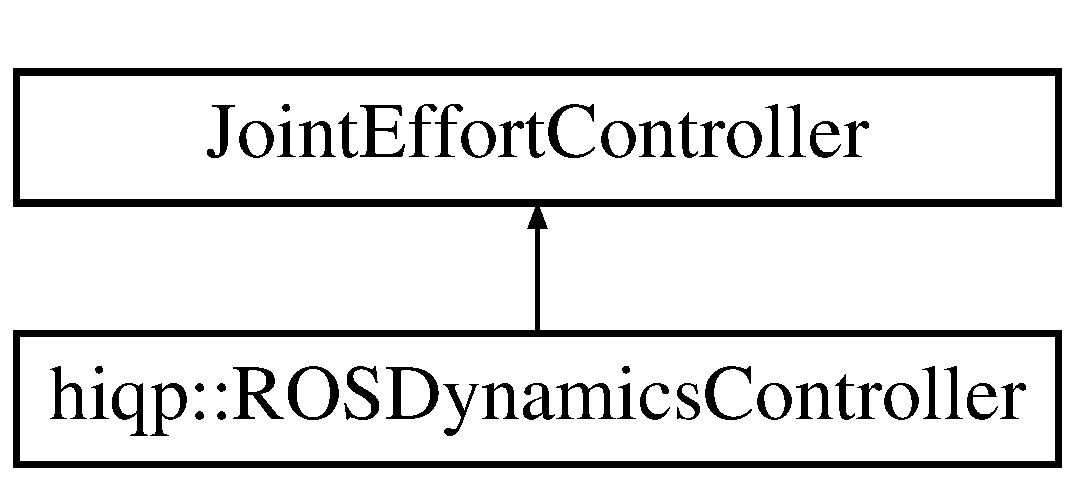
\includegraphics[height=2.000000cm]{classhiqp_1_1ROSDynamicsController}
\end{center}
\end{figure}
\subsection*{Public Member Functions}
\begin{DoxyCompactItemize}
\item 
\hypertarget{classhiqp_1_1ROSDynamicsController_ab25caf17b0f140092447b5209eb7ddd4}{\hyperlink{classhiqp_1_1ROSDynamicsController_ab25caf17b0f140092447b5209eb7ddd4}{R\-O\-S\-Dynamics\-Controller} ()}\label{classhiqp_1_1ROSDynamicsController_ab25caf17b0f140092447b5209eb7ddd4}

\begin{DoxyCompactList}\small\item\em Constructor Constructs my awesome controller. \end{DoxyCompactList}\item 
\hypertarget{classhiqp_1_1ROSDynamicsController_a007a61fdaa35652378b259ceb971d409}{\hyperlink{classhiqp_1_1ROSDynamicsController_a007a61fdaa35652378b259ceb971d409}{$\sim$\-R\-O\-S\-Dynamics\-Controller} () noexcept}\label{classhiqp_1_1ROSDynamicsController_a007a61fdaa35652378b259ceb971d409}

\begin{DoxyCompactList}\small\item\em Destructor Destructs my awesome controller \-:(. \end{DoxyCompactList}\item 
bool \hyperlink{classhiqp_1_1ROSDynamicsController_a2308da73670325884a035055bb86b7d2}{init} (\hyperlink{namespacehiqp_ac536ca3b4ba33489281fa5bec490799c}{Joint\-Velocity\-Interface} $\ast$hw, ros\-::\-Node\-Handle \&controller\-\_\-nh)
\begin{DoxyCompactList}\small\item\em Called every time the controller is initialized by the ros\-::controller\-\_\-manager. \end{DoxyCompactList}\item 
void \hyperlink{classhiqp_1_1ROSDynamicsController_aba55c2ae7df27d53ef5997ce51898ec0}{starting} (const ros\-::\-Time \&time)
\begin{DoxyCompactList}\small\item\em Called every time the controller is started by the ros\-::controller\-\_\-manager. \end{DoxyCompactList}\item 
void \hyperlink{classhiqp_1_1ROSDynamicsController_a369911a027a38555eff59bf838a8a7dd}{update} (const ros\-::\-Time \&time, const ros\-::\-Duration \&period)
\begin{DoxyCompactList}\small\item\em Called every time the controller is updated by the ros\-::controller\-\_\-manager. \end{DoxyCompactList}\item 
void \hyperlink{classhiqp_1_1ROSDynamicsController_aa8305ffc7cfd4eb1727e2133fc37aef9}{stopping} (const ros\-::\-Time \&time)
\begin{DoxyCompactList}\small\item\em Called every time the controller is stopped by the ros\-::controller\-\_\-manager. \end{DoxyCompactList}\end{DoxyCompactItemize}


\subsection{Detailed Description}
This is my awesome controller. 

It's awesome! 

\subsection{Member Function Documentation}
\hypertarget{classhiqp_1_1ROSDynamicsController_a2308da73670325884a035055bb86b7d2}{\index{hiqp\-::\-R\-O\-S\-Dynamics\-Controller@{hiqp\-::\-R\-O\-S\-Dynamics\-Controller}!init@{init}}
\index{init@{init}!hiqp::ROSDynamicsController@{hiqp\-::\-R\-O\-S\-Dynamics\-Controller}}
\subsubsection[{init}]{\setlength{\rightskip}{0pt plus 5cm}bool hiqp\-::\-R\-O\-S\-Dynamics\-Controller\-::init (
\begin{DoxyParamCaption}
\item[{{\bf Joint\-Velocity\-Interface} $\ast$}]{hw, }
\item[{ros\-::\-Node\-Handle \&}]{controller\-\_\-nh}
\end{DoxyParamCaption}
)}}\label{classhiqp_1_1ROSDynamicsController_a2308da73670325884a035055bb86b7d2}


Called every time the controller is initialized by the ros\-::controller\-\_\-manager. 

Does some cool stuff!


\begin{DoxyParams}{Parameters}
{\em hw} & \-: a pointer to the hardware interface used by this controller \\
\hline
{\em controller\-\_\-nh} & \-: the node handle of this controller \\
\hline
\end{DoxyParams}
\begin{DoxyReturn}{Returns}
true if the initialization was successful 
\end{DoxyReturn}
\hypertarget{classhiqp_1_1ROSDynamicsController_aba55c2ae7df27d53ef5997ce51898ec0}{\index{hiqp\-::\-R\-O\-S\-Dynamics\-Controller@{hiqp\-::\-R\-O\-S\-Dynamics\-Controller}!starting@{starting}}
\index{starting@{starting}!hiqp::ROSDynamicsController@{hiqp\-::\-R\-O\-S\-Dynamics\-Controller}}
\subsubsection[{starting}]{\setlength{\rightskip}{0pt plus 5cm}void hiqp\-::\-R\-O\-S\-Dynamics\-Controller\-::starting (
\begin{DoxyParamCaption}
\item[{const ros\-::\-Time \&}]{time}
\end{DoxyParamCaption}
)}}\label{classhiqp_1_1ROSDynamicsController_aba55c2ae7df27d53ef5997ce51898ec0}


Called every time the controller is started by the ros\-::controller\-\_\-manager. 

Does some cool stuff!


\begin{DoxyParams}{Parameters}
{\em time} & \-: the current wall-\/time in R\-O\-S \\
\hline
\end{DoxyParams}
\begin{DoxyReturn}{Returns}
true if the starting was successful 
\end{DoxyReturn}
\hypertarget{classhiqp_1_1ROSDynamicsController_aa8305ffc7cfd4eb1727e2133fc37aef9}{\index{hiqp\-::\-R\-O\-S\-Dynamics\-Controller@{hiqp\-::\-R\-O\-S\-Dynamics\-Controller}!stopping@{stopping}}
\index{stopping@{stopping}!hiqp::ROSDynamicsController@{hiqp\-::\-R\-O\-S\-Dynamics\-Controller}}
\subsubsection[{stopping}]{\setlength{\rightskip}{0pt plus 5cm}void hiqp\-::\-R\-O\-S\-Dynamics\-Controller\-::stopping (
\begin{DoxyParamCaption}
\item[{const ros\-::\-Time \&}]{time}
\end{DoxyParamCaption}
)}}\label{classhiqp_1_1ROSDynamicsController_aa8305ffc7cfd4eb1727e2133fc37aef9}


Called every time the controller is stopped by the ros\-::controller\-\_\-manager. 

Does some cool stuff!


\begin{DoxyParams}{Parameters}
{\em time} & \-: the current wall-\/time in R\-O\-S \\
\hline
\end{DoxyParams}
\begin{DoxyReturn}{Returns}
true if the stopping was successful 
\end{DoxyReturn}
\hypertarget{classhiqp_1_1ROSDynamicsController_a369911a027a38555eff59bf838a8a7dd}{\index{hiqp\-::\-R\-O\-S\-Dynamics\-Controller@{hiqp\-::\-R\-O\-S\-Dynamics\-Controller}!update@{update}}
\index{update@{update}!hiqp::ROSDynamicsController@{hiqp\-::\-R\-O\-S\-Dynamics\-Controller}}
\subsubsection[{update}]{\setlength{\rightskip}{0pt plus 5cm}void hiqp\-::\-R\-O\-S\-Dynamics\-Controller\-::update (
\begin{DoxyParamCaption}
\item[{const ros\-::\-Time \&}]{time, }
\item[{const ros\-::\-Duration \&}]{period}
\end{DoxyParamCaption}
)}}\label{classhiqp_1_1ROSDynamicsController_a369911a027a38555eff59bf838a8a7dd}


Called every time the controller is updated by the ros\-::controller\-\_\-manager. 

The function\-: 
\begin{DoxyEnumerate}
\item locks a mutex and reads position and velocity values from the joint handles, 
\item calls get\-Kinematic\-Controls() on its task manager, 
\item and locks a mutex and writes velocity values to the joint handles. 
\end{DoxyEnumerate}The joint handles are stored as a map between the joints q-\/number in the K\-D\-L\-::\-Tree and the joint handles themselves.


\begin{DoxyParams}{Parameters}
{\em time} & \-: the current wall-\/time in R\-O\-S \\
\hline
{\em period} & \-: the time between the last update call and this, i.\-e. the sample time. \\
\hline
\end{DoxyParams}
\begin{DoxyReturn}{Returns}
true if the update was successful 
\end{DoxyReturn}


The documentation for this class was generated from the following file\-:\begin{DoxyCompactItemize}
\item 
include/hiqp/ros\-\_\-dynamics\-\_\-controller.\-h\end{DoxyCompactItemize}

\hypertarget{classROSKinematicController}{\section{R\-O\-S\-Kinematic\-Controller Class Reference}
\label{classROSKinematicController}\index{R\-O\-S\-Kinematic\-Controller@{R\-O\-S\-Kinematic\-Controller}}
}


This is my awesome controller.  




{\ttfamily \#include $<$ros\-\_\-kinematics\-\_\-controller.\-h$>$}



\subsection{Detailed Description}
This is my awesome controller. 

It's awesome! 

The documentation for this class was generated from the following file\-:\begin{DoxyCompactItemize}
\item 
include/hiqp/\hyperlink{ros__kinematics__controller_8h}{ros\-\_\-kinematics\-\_\-controller.\-h}\end{DoxyCompactItemize}

\hypertarget{classhiqp_1_1ROSKinematicsController}{\section{hiqp\-:\-:R\-O\-S\-Kinematics\-Controller Class Reference}
\label{classhiqp_1_1ROSKinematicsController}\index{hiqp\-::\-R\-O\-S\-Kinematics\-Controller@{hiqp\-::\-R\-O\-S\-Kinematics\-Controller}}
}


A velocity controller compatible with R\-O\-S that uses the Hi\-Q\-P control framework.  




{\ttfamily \#include $<$ros\-\_\-kinematics\-\_\-controller.\-h$>$}

Inheritance diagram for hiqp\-:\-:R\-O\-S\-Kinematics\-Controller\-:\begin{figure}[H]
\begin{center}
\leavevmode
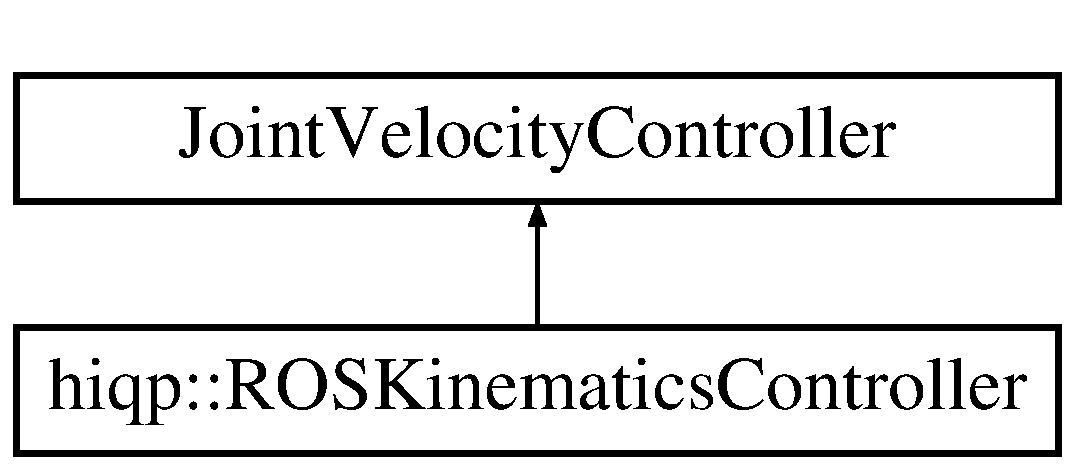
\includegraphics[height=2.000000cm]{classhiqp_1_1ROSKinematicsController}
\end{center}
\end{figure}
\subsection*{Public Member Functions}
\begin{DoxyCompactItemize}
\item 
bool \hyperlink{classhiqp_1_1ROSKinematicsController_a9acc590f4c514c1321f95f0667d1aae0}{init} (Joint\-Velocity\-Interface $\ast$hw, ros\-::\-Node\-Handle \&controller\-\_\-nh)
\begin{DoxyCompactList}\small\item\em Called every time the controller is initialized by the ros\-::controller\-\_\-manager. \end{DoxyCompactList}\item 
void \hyperlink{classhiqp_1_1ROSKinematicsController_a216a9b24cbb343496614d027868af72e}{starting} (const ros\-::\-Time \&time)
\begin{DoxyCompactList}\small\item\em Called every time the controller is started by the ros\-::controller\-\_\-manager. \end{DoxyCompactList}\item 
void \hyperlink{classhiqp_1_1ROSKinematicsController_aa4cc3905801b4097916731d0d7af2089}{update} (const ros\-::\-Time \&time, const ros\-::\-Duration \&period)
\begin{DoxyCompactList}\small\item\em Called every time the controller is updated by the ros\-::controller\-\_\-manager. \end{DoxyCompactList}\item 
void \hyperlink{classhiqp_1_1ROSKinematicsController_a683aa002bcca543a308e2a8ab507cfa5}{stopping} (const ros\-::\-Time \&time)
\begin{DoxyCompactList}\small\item\em Called every time the controller is stopped by the ros\-::controller\-\_\-manager. \end{DoxyCompactList}\end{DoxyCompactItemize}


\subsection{Detailed Description}
A velocity controller compatible with R\-O\-S that uses the Hi\-Q\-P control framework. 

\subsection{Member Function Documentation}
\hypertarget{classhiqp_1_1ROSKinematicsController_a9acc590f4c514c1321f95f0667d1aae0}{\index{hiqp\-::\-R\-O\-S\-Kinematics\-Controller@{hiqp\-::\-R\-O\-S\-Kinematics\-Controller}!init@{init}}
\index{init@{init}!hiqp::ROSKinematicsController@{hiqp\-::\-R\-O\-S\-Kinematics\-Controller}}
\subsubsection[{init}]{\setlength{\rightskip}{0pt plus 5cm}bool hiqp\-::\-R\-O\-S\-Kinematics\-Controller\-::init (
\begin{DoxyParamCaption}
\item[{Joint\-Velocity\-Interface $\ast$}]{hw, }
\item[{ros\-::\-Node\-Handle \&}]{controller\-\_\-nh}
\end{DoxyParamCaption}
)}}\label{classhiqp_1_1ROSKinematicsController_a9acc590f4c514c1321f95f0667d1aae0}


Called every time the controller is initialized by the ros\-::controller\-\_\-manager. 

Does some cool stuff!


\begin{DoxyParams}{Parameters}
{\em hw} & \-: a pointer to the hardware interface used by this controller \\
\hline
{\em controller\-\_\-nh} & \-: the node handle of this controller \\
\hline
\end{DoxyParams}
\begin{DoxyReturn}{Returns}
true if the initialization was successful 
\end{DoxyReturn}
\hypertarget{classhiqp_1_1ROSKinematicsController_a216a9b24cbb343496614d027868af72e}{\index{hiqp\-::\-R\-O\-S\-Kinematics\-Controller@{hiqp\-::\-R\-O\-S\-Kinematics\-Controller}!starting@{starting}}
\index{starting@{starting}!hiqp::ROSKinematicsController@{hiqp\-::\-R\-O\-S\-Kinematics\-Controller}}
\subsubsection[{starting}]{\setlength{\rightskip}{0pt plus 5cm}void hiqp\-::\-R\-O\-S\-Kinematics\-Controller\-::starting (
\begin{DoxyParamCaption}
\item[{const ros\-::\-Time \&}]{time}
\end{DoxyParamCaption}
)}}\label{classhiqp_1_1ROSKinematicsController_a216a9b24cbb343496614d027868af72e}


Called every time the controller is started by the ros\-::controller\-\_\-manager. 

Does some cool stuff!


\begin{DoxyParams}{Parameters}
{\em time} & \-: the current wall-\/time in R\-O\-S \\
\hline
\end{DoxyParams}
\begin{DoxyReturn}{Returns}
true if the starting was successful 
\end{DoxyReturn}
\hypertarget{classhiqp_1_1ROSKinematicsController_a683aa002bcca543a308e2a8ab507cfa5}{\index{hiqp\-::\-R\-O\-S\-Kinematics\-Controller@{hiqp\-::\-R\-O\-S\-Kinematics\-Controller}!stopping@{stopping}}
\index{stopping@{stopping}!hiqp::ROSKinematicsController@{hiqp\-::\-R\-O\-S\-Kinematics\-Controller}}
\subsubsection[{stopping}]{\setlength{\rightskip}{0pt plus 5cm}void hiqp\-::\-R\-O\-S\-Kinematics\-Controller\-::stopping (
\begin{DoxyParamCaption}
\item[{const ros\-::\-Time \&}]{time}
\end{DoxyParamCaption}
)}}\label{classhiqp_1_1ROSKinematicsController_a683aa002bcca543a308e2a8ab507cfa5}


Called every time the controller is stopped by the ros\-::controller\-\_\-manager. 

Does some cool stuff!


\begin{DoxyParams}{Parameters}
{\em time} & \-: the current wall-\/time in R\-O\-S \\
\hline
\end{DoxyParams}
\begin{DoxyReturn}{Returns}
true if the stopping was successful 
\end{DoxyReturn}
\hypertarget{classhiqp_1_1ROSKinematicsController_aa4cc3905801b4097916731d0d7af2089}{\index{hiqp\-::\-R\-O\-S\-Kinematics\-Controller@{hiqp\-::\-R\-O\-S\-Kinematics\-Controller}!update@{update}}
\index{update@{update}!hiqp::ROSKinematicsController@{hiqp\-::\-R\-O\-S\-Kinematics\-Controller}}
\subsubsection[{update}]{\setlength{\rightskip}{0pt plus 5cm}void hiqp\-::\-R\-O\-S\-Kinematics\-Controller\-::update (
\begin{DoxyParamCaption}
\item[{const ros\-::\-Time \&}]{time, }
\item[{const ros\-::\-Duration \&}]{period}
\end{DoxyParamCaption}
)}}\label{classhiqp_1_1ROSKinematicsController_aa4cc3905801b4097916731d0d7af2089}


Called every time the controller is updated by the ros\-::controller\-\_\-manager. 

The function\-: 
\begin{DoxyEnumerate}
\item locks a mutex and reads position and velocity values from the joint handles, 
\item calls get\-Kinematic\-Controls() on its task manager, 
\item and locks a mutex and writes velocity values to the joint handles. 
\end{DoxyEnumerate}The joint handles are stored as a map between the joints q-\/number in the K\-D\-L\-::\-Tree and the joint handles themselves.


\begin{DoxyParams}{Parameters}
{\em time} & \-: the current wall-\/time in R\-O\-S \\
\hline
{\em period} & \-: the time between the last update call and this, i.\-e. the sample time. \\
\hline
\end{DoxyParams}
\begin{DoxyReturn}{Returns}
true if the update was successful 
\end{DoxyReturn}


The documentation for this class was generated from the following files\-:\begin{DoxyCompactItemize}
\item 
include/hiqp/ros\-\_\-kinematics\-\_\-controller.\-h\item 
src/ros\-\_\-kinematics\-\_\-controller.\-cpp\end{DoxyCompactItemize}

\hypertarget{classhiqp_1_1ROSTopicSubscriber}{\section{hiqp\-:\-:R\-O\-S\-Topic\-Subscriber Class Reference}
\label{classhiqp_1_1ROSTopicSubscriber}\index{hiqp\-::\-R\-O\-S\-Topic\-Subscriber@{hiqp\-::\-R\-O\-S\-Topic\-Subscriber}}
}
\subsection*{Public Member Functions}
\begin{DoxyCompactItemize}
\item 
\hypertarget{classhiqp_1_1ROSTopicSubscriber_a16243f65f126f01b3fd7663037a73f87}{int {\bfseries init} (Geometric\-Primitive\-Map $\ast$primitive\-\_\-map)}\label{classhiqp_1_1ROSTopicSubscriber_a16243f65f126f01b3fd7663037a73f87}

\item 
\hypertarget{classhiqp_1_1ROSTopicSubscriber_a49bb3142efc3c4219f873d6d40cc9ae5}{{\footnotesize template$<$typename R\-O\-S\-Message\-Type $>$ }\\int {\bfseries add\-Subscription} (ros\-::\-Node\-Handle \&controller\-\_\-nh, const std\-::string \&topic\-\_\-name, unsigned int buffer\-\_\-size)}\label{classhiqp_1_1ROSTopicSubscriber_a49bb3142efc3c4219f873d6d40cc9ae5}

\item 
\hypertarget{classhiqp_1_1ROSTopicSubscriber_addcc31d45f31fdfb386a8e1b437ef3db}{{\footnotesize template$<$typename R\-O\-S\-Message\-Type $>$ }\\void \hyperlink{classhiqp_1_1ROSTopicSubscriber_addcc31d45f31fdfb386a8e1b437ef3db}{topic\-Callback} (const R\-O\-S\-Message\-Type \&msg)}\label{classhiqp_1_1ROSTopicSubscriber_addcc31d45f31fdfb386a8e1b437ef3db}

\begin{DoxyCompactList}\small\item\em Implement this function for your own message! \end{DoxyCompactList}\end{DoxyCompactItemize}


The documentation for this class was generated from the following file\-:\begin{DoxyCompactItemize}
\item 
include/hiqp/ros\-\_\-topic\-\_\-subscriber.\-h\end{DoxyCompactItemize}

\hypertarget{classhiqp_1_1ROSVisualizer}{\section{hiqp\-:\-:R\-O\-S\-Visualizer Class Reference}
\label{classhiqp_1_1ROSVisualizer}\index{hiqp\-::\-R\-O\-S\-Visualizer@{hiqp\-::\-R\-O\-S\-Visualizer}}
}
Inheritance diagram for hiqp\-:\-:R\-O\-S\-Visualizer\-:\begin{figure}[H]
\begin{center}
\leavevmode
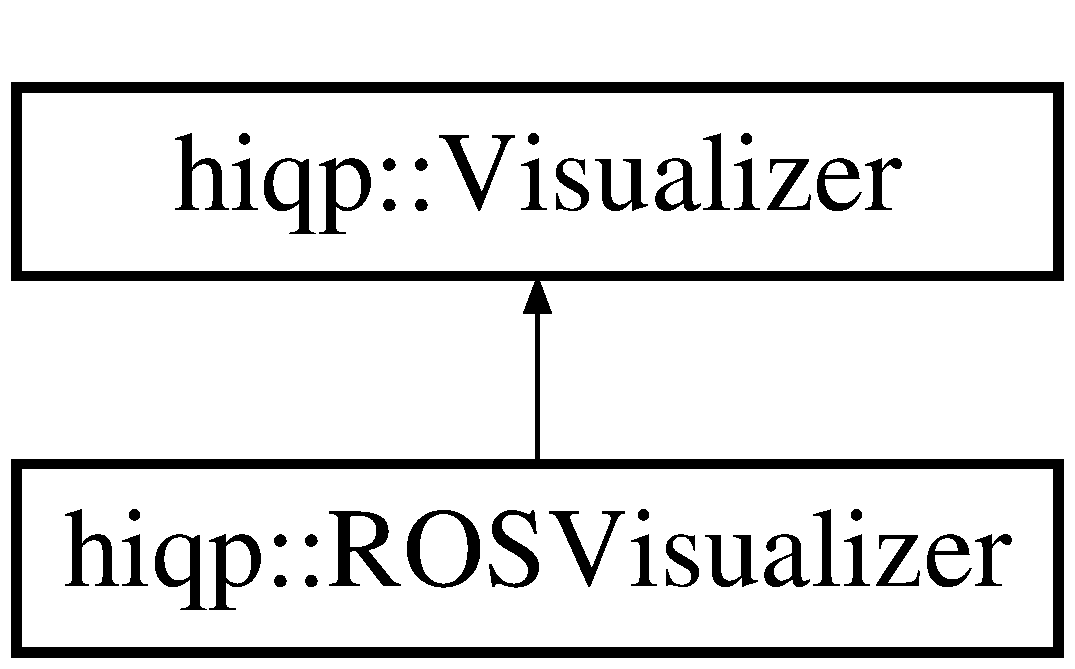
\includegraphics[height=2.000000cm]{classhiqp_1_1ROSVisualizer}
\end{center}
\end{figure}
\subsection*{Public Member Functions}
\begin{DoxyCompactItemize}
\item 
\hypertarget{classhiqp_1_1ROSVisualizer_a942a1082ce52a9831c40003667cabca5}{int {\bfseries init} (ros\-::\-Node\-Handle $\ast$controller\-\_\-nh)}\label{classhiqp_1_1ROSVisualizer_a942a1082ce52a9831c40003667cabca5}

\item 
\hypertarget{classhiqp_1_1ROSVisualizer_a554645f9016beb3a8471a8d61e5d9af1}{int {\bfseries add} (Geometric\-Point $\ast$point)}\label{classhiqp_1_1ROSVisualizer_a554645f9016beb3a8471a8d61e5d9af1}

\item 
\hypertarget{classhiqp_1_1ROSVisualizer_af3869b854ab72ef82ea0f96acd07f056}{int {\bfseries add} (Geometric\-Line $\ast$line)}\label{classhiqp_1_1ROSVisualizer_af3869b854ab72ef82ea0f96acd07f056}

\item 
\hypertarget{classhiqp_1_1ROSVisualizer_a1f3ce8e21494916060fb6b7d8f328717}{int {\bfseries add} (Geometric\-Plane $\ast$plane)}\label{classhiqp_1_1ROSVisualizer_a1f3ce8e21494916060fb6b7d8f328717}

\item 
\hypertarget{classhiqp_1_1ROSVisualizer_a0dab1fa740a8f29cded1299dc901476b}{int {\bfseries add} (Geometric\-Box $\ast$box)}\label{classhiqp_1_1ROSVisualizer_a0dab1fa740a8f29cded1299dc901476b}

\item 
\hypertarget{classhiqp_1_1ROSVisualizer_ab79b7a9a546c8258b7705e2170c5a6b0}{int {\bfseries add} (Geometric\-Cylinder $\ast$cylinder)}\label{classhiqp_1_1ROSVisualizer_ab79b7a9a546c8258b7705e2170c5a6b0}

\item 
\hypertarget{classhiqp_1_1ROSVisualizer_ada15c36e1a0f241b2869bf81e2da2afe}{int {\bfseries add} (Geometric\-Sphere $\ast$sphere)}\label{classhiqp_1_1ROSVisualizer_ada15c36e1a0f241b2869bf81e2da2afe}

\item 
\hypertarget{classhiqp_1_1ROSVisualizer_a8c04c3c3eb169738f1e0f1b7beed5745}{void {\bfseries update} (int id, Geometric\-Point $\ast$point)}\label{classhiqp_1_1ROSVisualizer_a8c04c3c3eb169738f1e0f1b7beed5745}

\item 
\hypertarget{classhiqp_1_1ROSVisualizer_ad28ab7953d60646399ef60aaf0f1e3fc}{void {\bfseries update} (int id, Geometric\-Line $\ast$line)}\label{classhiqp_1_1ROSVisualizer_ad28ab7953d60646399ef60aaf0f1e3fc}

\item 
\hypertarget{classhiqp_1_1ROSVisualizer_a2bd65ada4695ff3f8c3a10c6933443bf}{void {\bfseries update} (int id, Geometric\-Plane $\ast$plane)}\label{classhiqp_1_1ROSVisualizer_a2bd65ada4695ff3f8c3a10c6933443bf}

\item 
\hypertarget{classhiqp_1_1ROSVisualizer_a5c08aa488a28bc7661f042b1ec5120c1}{void {\bfseries update} (int id, Geometric\-Box $\ast$box)}\label{classhiqp_1_1ROSVisualizer_a5c08aa488a28bc7661f042b1ec5120c1}

\item 
\hypertarget{classhiqp_1_1ROSVisualizer_a004e1e446200c1d006c04b8417d6db00}{void {\bfseries update} (int id, Geometric\-Cylinder $\ast$cylinder)}\label{classhiqp_1_1ROSVisualizer_a004e1e446200c1d006c04b8417d6db00}

\item 
\hypertarget{classhiqp_1_1ROSVisualizer_ae27ff3c9c44a2e0cffe068b6cbde3a88}{void {\bfseries update} (int id, Geometric\-Sphere $\ast$sphere)}\label{classhiqp_1_1ROSVisualizer_ae27ff3c9c44a2e0cffe068b6cbde3a88}

\item 
\hypertarget{classhiqp_1_1ROSVisualizer_acfd8f9c92e114cee0c8207255b7126e7}{void {\bfseries remove} (int id)}\label{classhiqp_1_1ROSVisualizer_acfd8f9c92e114cee0c8207255b7126e7}

\item 
\hypertarget{classhiqp_1_1ROSVisualizer_a180827433d3c547c9d8afabb95694c5d}{void {\bfseries remove\-Many} (const std\-::vector$<$ int $>$ \&ids)}\label{classhiqp_1_1ROSVisualizer_a180827433d3c547c9d8afabb95694c5d}

\end{DoxyCompactItemize}


The documentation for this class was generated from the following files\-:\begin{DoxyCompactItemize}
\item 
include/hiqp/\hyperlink{ros__visualizer_8h}{ros\-\_\-visualizer.\-h}\item 
src/\hyperlink{ros__visualizer_8cpp}{ros\-\_\-visualizer.\-cpp}\end{DoxyCompactItemize}

\hypertarget{classhiqp_1_1TaskDynamics}{\section{hiqp\-:\-:Task\-Dynamics Class Reference}
\label{classhiqp_1_1TaskDynamics}\index{hiqp\-::\-Task\-Dynamics@{hiqp\-::\-Task\-Dynamics}}
}
Inheritance diagram for hiqp\-:\-:Task\-Dynamics\-:\begin{figure}[H]
\begin{center}
\leavevmode
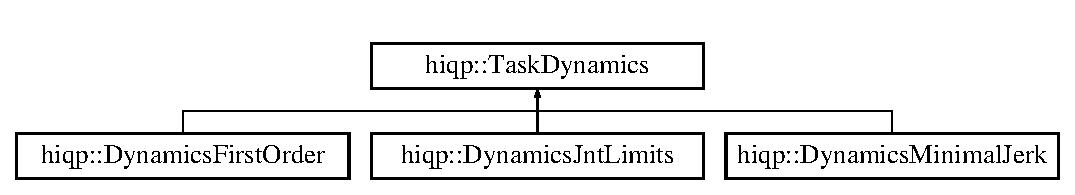
\includegraphics[height=2.000000cm]{classhiqp_1_1TaskDynamics}
\end{center}
\end{figure}
\subsection*{Public Member Functions}
\begin{DoxyCompactItemize}
\item 
\hypertarget{classhiqp_1_1TaskDynamics_a40d177e44645d0188f44788bde0adba0}{virtual int {\bfseries init} (const \hyperlink{classhiqp_1_1HiQPTimePoint}{Hi\-Q\-P\-Time\-Point} \&sampling\-\_\-time, const std\-::vector$<$ std\-::string $>$ \&parameters, const Eigen\-::\-Vector\-Xd \&e\-\_\-initial, const Eigen\-::\-Vector\-Xd \&e\-\_\-final)=0}\label{classhiqp_1_1TaskDynamics_a40d177e44645d0188f44788bde0adba0}

\item 
\hypertarget{classhiqp_1_1TaskDynamics_a12685734a0307147bcc453bd315a32f0}{virtual int {\bfseries apply} (const \hyperlink{classhiqp_1_1HiQPTimePoint}{Hi\-Q\-P\-Time\-Point} \&sampling\-\_\-time, const Eigen\-::\-Vector\-Xd \&e, const Eigen\-::\-Matrix\-Xd \&J, Eigen\-::\-Vector\-Xd \&e\-\_\-dot\-\_\-star)=0}\label{classhiqp_1_1TaskDynamics_a12685734a0307147bcc453bd315a32f0}

\item 
\hypertarget{classhiqp_1_1TaskDynamics_a1ab7af71fd1774068e540656dc00af49}{virtual int {\bfseries monitor} ()=0}\label{classhiqp_1_1TaskDynamics_a1ab7af71fd1774068e540656dc00af49}

\item 
\hypertarget{classhiqp_1_1TaskDynamics_a68dc5c02721b9665bb5e49a8a0a5cadc}{const std\-::string \& {\bfseries get\-Dynamics\-Type\-Name} ()}\label{classhiqp_1_1TaskDynamics_a68dc5c02721b9665bb5e49a8a0a5cadc}

\end{DoxyCompactItemize}
\subsection*{Protected Attributes}
\begin{DoxyCompactItemize}
\item 
\hypertarget{classhiqp_1_1TaskDynamics_acbef47a5ae066079eb530aa0d6b02569}{std\-::vector$<$ double $>$ {\bfseries performance\-\_\-measures\-\_\-}}\label{classhiqp_1_1TaskDynamics_acbef47a5ae066079eb530aa0d6b02569}

\end{DoxyCompactItemize}


The documentation for this class was generated from the following file\-:\begin{DoxyCompactItemize}
\item 
include/hiqp/\hyperlink{task__dynamics_8h}{task\-\_\-dynamics.\-h}\end{DoxyCompactItemize}

\hypertarget{classhiqp_1_1TaskFactory}{\section{hiqp\-:\-:Task\-Factory Class Reference}
\label{classhiqp_1_1TaskFactory}\index{hiqp\-::\-Task\-Factory@{hiqp\-::\-Task\-Factory}}
}


A factory for creating task function and task dynamics. (The process of creating and initializing them is intertwined.)  




{\ttfamily \#include $<$task\-\_\-factory.\-h$>$}

\subsection*{Public Member Functions}
\begin{DoxyCompactItemize}
\item 
\hypertarget{classhiqp_1_1TaskFactory_a18b39d326d787327514ec0fc73a155fd}{void {\bfseries init} (Geometric\-Primitive\-Map $\ast$geometric\-\_\-primitive\-\_\-map, \hyperlink{classhiqp_1_1Visualizer}{Visualizer} $\ast$visualizer, unsigned int num\-\_\-controls)}\label{classhiqp_1_1TaskFactory_a18b39d326d787327514ec0fc73a155fd}

\item 
\hypertarget{classhiqp_1_1TaskFactory_a3afab0c3567f34f7407249f6bf3a9b1f}{int {\bfseries build\-Task} (const std\-::string \&name, const std\-::string \&type, unsigned int priority, bool visibility, const std\-::vector$<$ std\-::string $>$ \&parameters, const std\-::vector$<$ std\-::string $>$ \&behaviour\-\_\-parameters, const \hyperlink{classhiqp_1_1HiQPTimePoint}{Hi\-Q\-P\-Time\-Point} \&sampling\-\_\-time, const K\-D\-L\-::\-Tree \&kdl\-\_\-tree, const K\-D\-L\-::\-Jnt\-Array\-Vel \&kdl\-\_\-joint\-\_\-pos\-\_\-vel, std\-::size\-\_\-t dynamics\-\_\-id, \hyperlink{classhiqp_1_1TaskDynamics}{Task\-Dynamics} $\ast$\&dynamics, \hyperlink{classhiqp_1_1TaskFunction}{Task\-Function} $\ast$\&function)}\label{classhiqp_1_1TaskFactory_a3afab0c3567f34f7407249f6bf3a9b1f}

\end{DoxyCompactItemize}


\subsection{Detailed Description}
A factory for creating task function and task dynamics. (The process of creating and initializing them is intertwined.) 

The documentation for this class was generated from the following files\-:\begin{DoxyCompactItemize}
\item 
include/hiqp/task\-\_\-factory.\-h\item 
src/task\-\_\-factory.\-cpp\end{DoxyCompactItemize}

\hypertarget{classhiqp_1_1TaskFullPose}{\section{hiqp\-:\-:Task\-Full\-Pose Class Reference}
\label{classhiqp_1_1TaskFullPose}\index{hiqp\-::\-Task\-Full\-Pose@{hiqp\-::\-Task\-Full\-Pose}}
}


Represents a task that sets a specific joint configuration.  




{\ttfamily \#include $<$task\-\_\-full\-\_\-pose.\-h$>$}

Inheritance diagram for hiqp\-:\-:Task\-Full\-Pose\-:\begin{figure}[H]
\begin{center}
\leavevmode
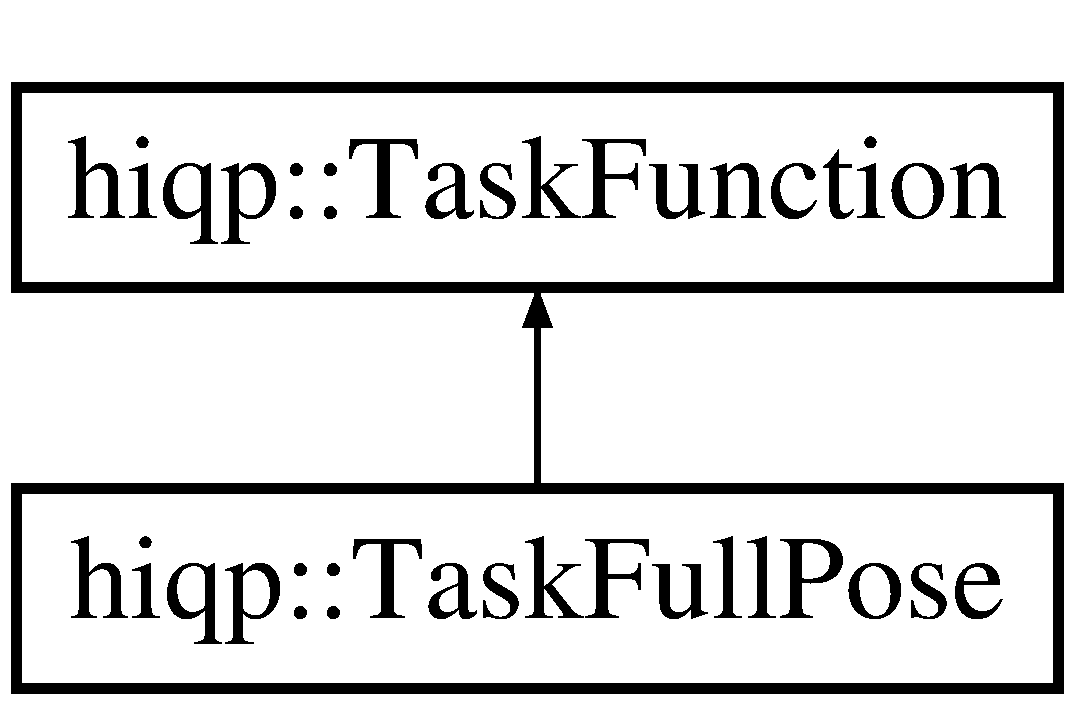
\includegraphics[height=2.000000cm]{classhiqp_1_1TaskFullPose}
\end{center}
\end{figure}
\subsection*{Public Member Functions}
\begin{DoxyCompactItemize}
\item 
\hypertarget{classhiqp_1_1TaskFullPose_a9791ec10bf86952b38726b4576dba015}{\hyperlink{classhiqp_1_1TaskFullPose_a9791ec10bf86952b38726b4576dba015}{Task\-Full\-Pose} ()}\label{classhiqp_1_1TaskFullPose_a9791ec10bf86952b38726b4576dba015}

\begin{DoxyCompactList}\small\item\em Constructor Constructs my awesome task. \end{DoxyCompactList}\item 
\hypertarget{classhiqp_1_1TaskFullPose_a88c4631a941fa37850919c8e87cf09a8}{\hyperlink{classhiqp_1_1TaskFullPose_a88c4631a941fa37850919c8e87cf09a8}{$\sim$\-Task\-Full\-Pose} () noexcept}\label{classhiqp_1_1TaskFullPose_a88c4631a941fa37850919c8e87cf09a8}

\begin{DoxyCompactList}\small\item\em Destructor Destructs my awesome task. \end{DoxyCompactList}\item 
int \hyperlink{classhiqp_1_1TaskFullPose_aed1a9b16310f7a7c991732701bd03ce0}{init} (const \hyperlink{classhiqp_1_1HiQPTimePoint}{Hi\-Q\-P\-Time\-Point} \&sampling\-\_\-time, const std\-::vector$<$ std\-::string $>$ \&parameters, const K\-D\-L\-::\-Tree \&kdl\-\_\-tree, unsigned int num\-\_\-controls)
\begin{DoxyCompactList}\small\item\em {\itshape Pure virtual}. Initializes the task \end{DoxyCompactList}\item 
int \hyperlink{classhiqp_1_1TaskFullPose_a7dcaa206ba1a24d205504ffaa3f55ac6}{apply} (const \hyperlink{classhiqp_1_1HiQPTimePoint}{Hi\-Q\-P\-Time\-Point} \&sampling\-\_\-time, const K\-D\-L\-::\-Tree \&kdl\-\_\-tree, const K\-D\-L\-::\-Jnt\-Array\-Vel \&kdl\-\_\-joint\-\_\-pos\-\_\-vel)
\begin{DoxyCompactList}\small\item\em {\itshape Pure virtual}. Calculates the task function and task jacobian values. \end{DoxyCompactList}\item 
int \hyperlink{classhiqp_1_1TaskFullPose_a46c3585f15b89f793b6a9debcb6e5db9}{monitor} ()
\begin{DoxyCompactList}\small\item\em Computes all performance measures used when monitoring this task. \end{DoxyCompactList}\end{DoxyCompactItemize}
\subsection*{Additional Inherited Members}


\subsection{Detailed Description}
Represents a task that sets a specific joint configuration. 

This task does not leave any redundancy available to other tasks. 

\subsection{Member Function Documentation}
\hypertarget{classhiqp_1_1TaskFullPose_a7dcaa206ba1a24d205504ffaa3f55ac6}{\index{hiqp\-::\-Task\-Full\-Pose@{hiqp\-::\-Task\-Full\-Pose}!apply@{apply}}
\index{apply@{apply}!hiqp::TaskFullPose@{hiqp\-::\-Task\-Full\-Pose}}
\subsubsection[{apply}]{\setlength{\rightskip}{0pt plus 5cm}int hiqp\-::\-Task\-Full\-Pose\-::apply (
\begin{DoxyParamCaption}
\item[{const {\bf Hi\-Q\-P\-Time\-Point} \&}]{sampling\-\_\-time, }
\item[{const K\-D\-L\-::\-Tree \&}]{kdl\-\_\-tree, }
\item[{const K\-D\-L\-::\-Jnt\-Array\-Vel \&}]{kdl\-\_\-joint\-\_\-pos\-\_\-vel}
\end{DoxyParamCaption}
)\hspace{0.3cm}{\ttfamily [virtual]}}}\label{classhiqp_1_1TaskFullPose_a7dcaa206ba1a24d205504ffaa3f55ac6}


{\itshape Pure virtual}. Calculates the task function and task jacobian values. 


\begin{DoxyParams}{Parameters}
{\em kdl\-\_\-tree} & \-: reference to the kinematic dynamic tree of the robot \\
\hline
{\em joints\-\_\-pos\-\_\-vel} & \-: reference to the current joint positions and velocities\\
\hline
\end{DoxyParams}
\begin{DoxyReturn}{Returns}
true if the calculation was successful 
\end{DoxyReturn}


Implements \hyperlink{classhiqp_1_1TaskFunction_a3c476e011c762b8a8f7470ec47f70a17}{hiqp\-::\-Task\-Function}.

\hypertarget{classhiqp_1_1TaskFullPose_aed1a9b16310f7a7c991732701bd03ce0}{\index{hiqp\-::\-Task\-Full\-Pose@{hiqp\-::\-Task\-Full\-Pose}!init@{init}}
\index{init@{init}!hiqp::TaskFullPose@{hiqp\-::\-Task\-Full\-Pose}}
\subsubsection[{init}]{\setlength{\rightskip}{0pt plus 5cm}int hiqp\-::\-Task\-Full\-Pose\-::init (
\begin{DoxyParamCaption}
\item[{const {\bf Hi\-Q\-P\-Time\-Point} \&}]{sampling\-\_\-time, }
\item[{const std\-::vector$<$ std\-::string $>$ \&}]{parameters, }
\item[{const K\-D\-L\-::\-Tree \&}]{kdl\-\_\-tree, }
\item[{unsigned int}]{num\-\_\-controls}
\end{DoxyParamCaption}
)\hspace{0.3cm}{\ttfamily [virtual]}}}\label{classhiqp_1_1TaskFullPose_aed1a9b16310f7a7c991732701bd03ce0}


{\itshape Pure virtual}. Initializes the task 

\begin{DoxyReturn}{Returns}
0 upon success 
\end{DoxyReturn}


Implements \hyperlink{classhiqp_1_1TaskFunction}{hiqp\-::\-Task\-Function}.

\hypertarget{classhiqp_1_1TaskFullPose_a46c3585f15b89f793b6a9debcb6e5db9}{\index{hiqp\-::\-Task\-Full\-Pose@{hiqp\-::\-Task\-Full\-Pose}!monitor@{monitor}}
\index{monitor@{monitor}!hiqp::TaskFullPose@{hiqp\-::\-Task\-Full\-Pose}}
\subsubsection[{monitor}]{\setlength{\rightskip}{0pt plus 5cm}int hiqp\-::\-Task\-Full\-Pose\-::monitor (
\begin{DoxyParamCaption}
{}
\end{DoxyParamCaption}
)\hspace{0.3cm}{\ttfamily [virtual]}}}\label{classhiqp_1_1TaskFullPose_a46c3585f15b89f793b6a9debcb6e5db9}


Computes all performance measures used when monitoring this task. 

\begin{DoxyReturn}{Returns}
0 if the calculation was successful 
\end{DoxyReturn}


Implements \hyperlink{classhiqp_1_1TaskFunction_a47a3283a0c0ebafa17feeca96afe5af0}{hiqp\-::\-Task\-Function}.



The documentation for this class was generated from the following files\-:\begin{DoxyCompactItemize}
\item 
include/hiqp/tasks/task\-\_\-full\-\_\-pose.\-h\item 
src/tasks/\hyperlink{task__full__pose_8cpp}{task\-\_\-full\-\_\-pose.\-cpp}\end{DoxyCompactItemize}

\hypertarget{classhiqp_1_1TaskFunction}{\section{hiqp\-:\-:Task\-Function Class Reference}
\label{classhiqp_1_1TaskFunction}\index{hiqp\-::\-Task\-Function@{hiqp\-::\-Task\-Function}}
}


Abstract base class for all task function types.  




{\ttfamily \#include $<$task\-\_\-function.\-h$>$}

Inheritance diagram for hiqp\-:\-:Task\-Function\-:\begin{figure}[H]
\begin{center}
\leavevmode
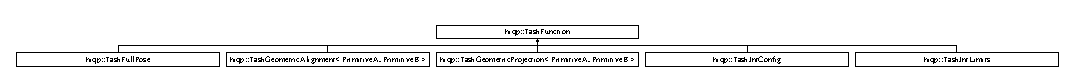
\includegraphics[height=0.607046cm]{classhiqp_1_1TaskFunction}
\end{center}
\end{figure}
\subsection*{Public Member Functions}
\begin{DoxyCompactItemize}
\item 
\hypertarget{classhiqp_1_1TaskFunction_a74b27f9f666988edb072fb8b6a790da3}{virtual int {\bfseries init} (const \hyperlink{classhiqp_1_1HiQPTimePoint}{Hi\-Q\-P\-Time\-Point} \&sampling\-\_\-time, const std\-::vector$<$ std\-::string $>$ \&parameters, const K\-D\-L\-::\-Tree \&kdl\-\_\-tree, unsigned int num\-\_\-controls)=0}\label{classhiqp_1_1TaskFunction_a74b27f9f666988edb072fb8b6a790da3}

\item 
virtual int \hyperlink{classhiqp_1_1TaskFunction_a3c476e011c762b8a8f7470ec47f70a17}{apply} (const \hyperlink{classhiqp_1_1HiQPTimePoint}{Hi\-Q\-P\-Time\-Point} \&sampling\-\_\-time, const K\-D\-L\-::\-Tree \&kdl\-\_\-tree, const K\-D\-L\-::\-Jnt\-Array\-Vel \&kdl\-\_\-joint\-\_\-pos\-\_\-vel)=0
\begin{DoxyCompactList}\small\item\em {\itshape Pure virtual}. Calculates the task function and task jacobian values. \end{DoxyCompactList}\item 
virtual int \hyperlink{classhiqp_1_1TaskFunction_a47a3283a0c0ebafa17feeca96afe5af0}{monitor} ()=0
\begin{DoxyCompactList}\small\item\em {\itshape Pure virtual}. Computes all performance measures used when monitoring this task. \end{DoxyCompactList}\item 
\hypertarget{classhiqp_1_1TaskFunction_a43f0634f321270ff9922985bc51992c0}{Eigen\-::\-Vector\-Xd {\bfseries get\-Initial\-State} ()}\label{classhiqp_1_1TaskFunction_a43f0634f321270ff9922985bc51992c0}

\item 
\hypertarget{classhiqp_1_1TaskFunction_a1450beadd7300ae786ff8c2756c94643}{Eigen\-::\-Matrix\-Xd {\bfseries get\-Initial\-State\-Jacobian} ()}\label{classhiqp_1_1TaskFunction_a1450beadd7300ae786ff8c2756c94643}

\item 
\hypertarget{classhiqp_1_1TaskFunction_a3869d4b73495e31ef63941b9cb95e55f}{virtual Eigen\-::\-Vector\-Xd {\bfseries get\-Final\-State} (const K\-D\-L\-::\-Tree \&kdl\-\_\-tree)}\label{classhiqp_1_1TaskFunction_a3869d4b73495e31ef63941b9cb95e55f}

\end{DoxyCompactItemize}
\subsection*{Protected Member Functions}
\begin{DoxyCompactItemize}
\item 
\hypertarget{classhiqp_1_1TaskFunction_ac6aec46978ac4162f69264d79e1c1ab8}{\hyperlink{classhiqp_1_1Visualizer}{Visualizer} $\ast$ {\bfseries get\-Visualizer} ()}\label{classhiqp_1_1TaskFunction_ac6aec46978ac4162f69264d79e1c1ab8}

\item 
\hypertarget{classhiqp_1_1TaskFunction_ab229de62c0f0c2b4620fd364d90c344f}{Geometric\-Primitive\-Map $\ast$ {\bfseries get\-Geometric\-Primitive\-Map} ()}\label{classhiqp_1_1TaskFunction_ab229de62c0f0c2b4620fd364d90c344f}

\item 
\hypertarget{classhiqp_1_1TaskFunction_a2af5e1230868e1949620c3e8bcf4de71}{std\-::size\-\_\-t {\bfseries get\-Dynamics\-Id} ()}\label{classhiqp_1_1TaskFunction_a2af5e1230868e1949620c3e8bcf4de71}

\item 
\hypertarget{classhiqp_1_1TaskFunction_a90ebccdc0bec19ec6379f2aaba2e3772}{const std\-::string \& {\bfseries get\-Task\-Name} ()}\label{classhiqp_1_1TaskFunction_a90ebccdc0bec19ec6379f2aaba2e3772}

\item 
\hypertarget{classhiqp_1_1TaskFunction_af5b3c489bb216aefb6e25db60a55eb0c}{const std\-::string \& {\bfseries get\-Task\-Type} ()}\label{classhiqp_1_1TaskFunction_af5b3c489bb216aefb6e25db60a55eb0c}

\item 
\hypertarget{classhiqp_1_1TaskFunction_a13f5da940c9bc2f7c669659b2b0a3cd4}{unsigned int {\bfseries get\-Priority} ()}\label{classhiqp_1_1TaskFunction_a13f5da940c9bc2f7c669659b2b0a3cd4}

\item 
\hypertarget{classhiqp_1_1TaskFunction_aa30289e417f880bbe41c0a0e2e3af362}{bool {\bfseries get\-Visibility} ()}\label{classhiqp_1_1TaskFunction_aa30289e417f880bbe41c0a0e2e3af362}

\end{DoxyCompactItemize}
\subsection*{Protected Attributes}
\begin{DoxyCompactItemize}
\item 
\hypertarget{classhiqp_1_1TaskFunction_add51e374b24c5179474709286b62a54d}{Eigen\-::\-Vector\-Xd {\bfseries e\-\_\-}}\label{classhiqp_1_1TaskFunction_add51e374b24c5179474709286b62a54d}

\item 
\hypertarget{classhiqp_1_1TaskFunction_ae0634f16b16eab8804cdef09ca2b8f34}{Eigen\-::\-Vector\-Xd {\bfseries e\-\_\-initial\-\_\-}}\label{classhiqp_1_1TaskFunction_ae0634f16b16eab8804cdef09ca2b8f34}

\item 
\hypertarget{classhiqp_1_1TaskFunction_a6799e07904601184a713b5f10039bc33}{Eigen\-::\-Matrix\-Xd {\bfseries J\-\_\-}}\label{classhiqp_1_1TaskFunction_a6799e07904601184a713b5f10039bc33}

\item 
\hypertarget{classhiqp_1_1TaskFunction_ae8920244fed253580ee68e1d97c0c1ea}{Eigen\-::\-Matrix\-Xd {\bfseries J\-\_\-initial\-\_\-}}\label{classhiqp_1_1TaskFunction_ae8920244fed253580ee68e1d97c0c1ea}

\item 
\hypertarget{classhiqp_1_1TaskFunction_a31661efda6f8cbb197e4b188c7ac070a}{Eigen\-::\-Vector\-Xd {\bfseries e\-\_\-dot\-\_\-star\-\_\-}}\label{classhiqp_1_1TaskFunction_a31661efda6f8cbb197e4b188c7ac070a}

\item 
\hypertarget{classhiqp_1_1TaskFunction_a3dbcd166e38dc81a4ab81a6f902688dd}{std\-::vector$<$ int $>$ {\bfseries task\-\_\-types\-\_\-}}\label{classhiqp_1_1TaskFunction_a3dbcd166e38dc81a4ab81a6f902688dd}

\item 
\hypertarget{classhiqp_1_1TaskFunction_ae3bf05a29068234cf202b80472f45c25}{std\-::vector$<$ double $>$ {\bfseries performance\-\_\-measures\-\_\-}}\label{classhiqp_1_1TaskFunction_ae3bf05a29068234cf202b80472f45c25}

\item 
\hypertarget{classhiqp_1_1TaskFunction_a815eff712a5d210e5c0ac3793ba93d7c}{std\-::vector$<$ double $>$ {\bfseries measures\-\_\-e\-\_\-}}\label{classhiqp_1_1TaskFunction_a815eff712a5d210e5c0ac3793ba93d7c}

\item 
\hypertarget{classhiqp_1_1TaskFunction_a5ce42f57c0e92a345b5da16142476f1a}{std\-::vector$<$ double $>$ {\bfseries measures\-\_\-e\-\_\-dot\-\_\-star\-\_\-}}\label{classhiqp_1_1TaskFunction_a5ce42f57c0e92a345b5da16142476f1a}

\item 
\hypertarget{classhiqp_1_1TaskFunction_a4ac63da941c91bc05733836bbaacb769}{std\-::vector$<$ double $>$ {\bfseries measures\-\_\-\-J\-\_\-}}\label{classhiqp_1_1TaskFunction_a4ac63da941c91bc05733836bbaacb769}

\item 
\hypertarget{classhiqp_1_1TaskFunction_a086192d37a36e72f781e9641cd35176d}{Geometric\-Primitive\-Map $\ast$ {\bfseries geometric\-\_\-primitive\-\_\-map\-\_\-}}\label{classhiqp_1_1TaskFunction_a086192d37a36e72f781e9641cd35176d}

\end{DoxyCompactItemize}


\subsection{Detailed Description}
Abstract base class for all task function types. 

\subsection{Member Function Documentation}
\hypertarget{classhiqp_1_1TaskFunction_a3c476e011c762b8a8f7470ec47f70a17}{\index{hiqp\-::\-Task\-Function@{hiqp\-::\-Task\-Function}!apply@{apply}}
\index{apply@{apply}!hiqp::TaskFunction@{hiqp\-::\-Task\-Function}}
\subsubsection[{apply}]{\setlength{\rightskip}{0pt plus 5cm}virtual int hiqp\-::\-Task\-Function\-::apply (
\begin{DoxyParamCaption}
\item[{const {\bf Hi\-Q\-P\-Time\-Point} \&}]{sampling\-\_\-time, }
\item[{const K\-D\-L\-::\-Tree \&}]{kdl\-\_\-tree, }
\item[{const K\-D\-L\-::\-Jnt\-Array\-Vel \&}]{kdl\-\_\-joint\-\_\-pos\-\_\-vel}
\end{DoxyParamCaption}
)\hspace{0.3cm}{\ttfamily [pure virtual]}}}\label{classhiqp_1_1TaskFunction_a3c476e011c762b8a8f7470ec47f70a17}


{\itshape Pure virtual}. Calculates the task function and task jacobian values. 


\begin{DoxyParams}{Parameters}
{\em kdl\-\_\-tree} & \-: reference to the kinematic dynamic tree of the robot \\
\hline
{\em kdl\-\_\-joint\-\_\-pos\-\_\-vel} & \-: reference to the current joint positions and velocities \\
\hline
{\em task\-\_\-fun\-\_\-val} & \-: reference to where the output controls are to be stored\\
\hline
\end{DoxyParams}
\begin{DoxyReturn}{Returns}
0 if the calculation was successful 
\end{DoxyReturn}


Implemented in \hyperlink{classhiqp_1_1tasks_1_1TaskFullPose_aa3f9600219741a8bb7ffcb15bba19c70}{hiqp\-::tasks\-::\-Task\-Full\-Pose}, \hyperlink{classhiqp_1_1tasks_1_1TaskGeometricAlignment_aa46e561c924dd0a65f463a715ed387a3}{hiqp\-::tasks\-::\-Task\-Geometric\-Alignment$<$ Primitive\-A, Primitive\-B $>$}, \hyperlink{classhiqp_1_1tasks_1_1TaskGeometricProjection_a80d6bb74fb3faae77a6ef3e141846761}{hiqp\-::tasks\-::\-Task\-Geometric\-Projection$<$ Primitive\-A, Primitive\-B $>$}, \hyperlink{classhiqp_1_1tasks_1_1TaskJntConfig_a5e5ed2b1a16a96fbdaff3e95fd1b2329}{hiqp\-::tasks\-::\-Task\-Jnt\-Config}, and \hyperlink{classhiqp_1_1tasks_1_1TaskJntLimits_a3ab9389dfc0e3646fbd1fd670d7285fe}{hiqp\-::tasks\-::\-Task\-Jnt\-Limits}.

\hypertarget{classhiqp_1_1TaskFunction_a47a3283a0c0ebafa17feeca96afe5af0}{\index{hiqp\-::\-Task\-Function@{hiqp\-::\-Task\-Function}!monitor@{monitor}}
\index{monitor@{monitor}!hiqp::TaskFunction@{hiqp\-::\-Task\-Function}}
\subsubsection[{monitor}]{\setlength{\rightskip}{0pt plus 5cm}virtual int hiqp\-::\-Task\-Function\-::monitor (
\begin{DoxyParamCaption}
{}
\end{DoxyParamCaption}
)\hspace{0.3cm}{\ttfamily [pure virtual]}}}\label{classhiqp_1_1TaskFunction_a47a3283a0c0ebafa17feeca96afe5af0}


{\itshape Pure virtual}. Computes all performance measures used when monitoring this task. 

\begin{DoxyReturn}{Returns}
0 if the calculation was successful 
\end{DoxyReturn}


Implemented in \hyperlink{classhiqp_1_1tasks_1_1TaskFullPose_a1280f9a08af7083c28fc31cf66a61f55}{hiqp\-::tasks\-::\-Task\-Full\-Pose}, \hyperlink{classhiqp_1_1tasks_1_1TaskGeometricAlignment_a1c01a7489e846175992a44a62a8a7436}{hiqp\-::tasks\-::\-Task\-Geometric\-Alignment$<$ Primitive\-A, Primitive\-B $>$}, \hyperlink{classhiqp_1_1tasks_1_1TaskGeometricProjection_a58d7416dfaa2ff0241065be68282848c}{hiqp\-::tasks\-::\-Task\-Geometric\-Projection$<$ Primitive\-A, Primitive\-B $>$}, \hyperlink{classhiqp_1_1tasks_1_1TaskJntConfig_a903a952db54532a9650c725141399774}{hiqp\-::tasks\-::\-Task\-Jnt\-Config}, and \hyperlink{classhiqp_1_1tasks_1_1TaskJntLimits_ace02732e6cd3cc4087baf6e7df5e2723}{hiqp\-::tasks\-::\-Task\-Jnt\-Limits}.



The documentation for this class was generated from the following file\-:\begin{DoxyCompactItemize}
\item 
include/hiqp/\hyperlink{task__function_8h}{task\-\_\-function.\-h}\end{DoxyCompactItemize}

\hypertarget{classhiqp_1_1TaskGeometricAlignment}{\section{hiqp\-:\-:Task\-Geometric\-Alignment$<$ Primitive\-A, Primitive\-B $>$ Class Template Reference}
\label{classhiqp_1_1TaskGeometricAlignment}\index{hiqp\-::\-Task\-Geometric\-Alignment$<$ Primitive\-A, Primitive\-B $>$@{hiqp\-::\-Task\-Geometric\-Alignment$<$ Primitive\-A, Primitive\-B $>$}}
}
Inheritance diagram for hiqp\-:\-:Task\-Geometric\-Alignment$<$ Primitive\-A, Primitive\-B $>$\-:\begin{figure}[H]
\begin{center}
\leavevmode
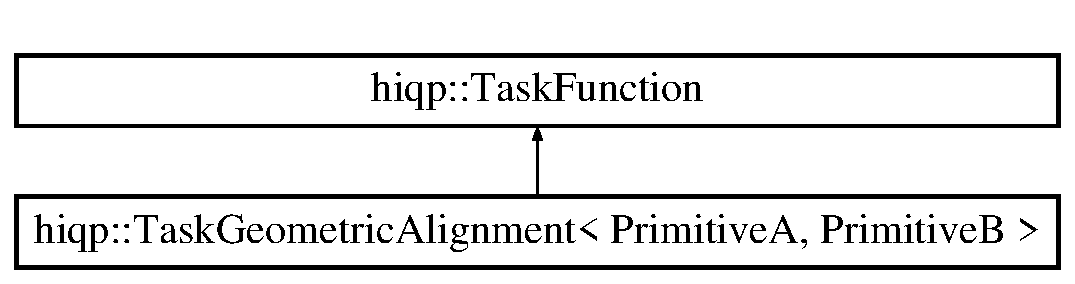
\includegraphics[height=2.000000cm]{classhiqp_1_1TaskGeometricAlignment}
\end{center}
\end{figure}
\subsection*{Public Member Functions}
\begin{DoxyCompactItemize}
\item 
\hypertarget{classhiqp_1_1TaskGeometricAlignment_a8f089ad7dab000f343341a159c61a0ca}{\hyperlink{classhiqp_1_1TaskGeometricAlignment_a8f089ad7dab000f343341a159c61a0ca}{Task\-Geometric\-Alignment} ()}\label{classhiqp_1_1TaskGeometricAlignment_a8f089ad7dab000f343341a159c61a0ca}

\begin{DoxyCompactList}\small\item\em Constructor. \end{DoxyCompactList}\item 
\hypertarget{classhiqp_1_1TaskGeometricAlignment_a94c787691eeafd7ca1f7979c54aa79e4}{\hyperlink{classhiqp_1_1TaskGeometricAlignment_a94c787691eeafd7ca1f7979c54aa79e4}{$\sim$\-Task\-Geometric\-Alignment} () noexcept}\label{classhiqp_1_1TaskGeometricAlignment_a94c787691eeafd7ca1f7979c54aa79e4}

\begin{DoxyCompactList}\small\item\em Destructor. \end{DoxyCompactList}\item 
int \hyperlink{classhiqp_1_1TaskGeometricAlignment_a532c586ac698619c0f2d18fe44253bec}{init} (const \hyperlink{classhiqp_1_1HiQPTimePoint}{Hi\-Q\-P\-Time\-Point} \&sampling\-\_\-time, const std\-::vector$<$ std\-::string $>$ \&parameters, const K\-D\-L\-::\-Tree \&kdl\-\_\-tree, unsigned int num\-\_\-controls)
\begin{DoxyCompactList}\small\item\em Initializes the task. \end{DoxyCompactList}\item 
int \hyperlink{classhiqp_1_1TaskGeometricAlignment_a85bec9aead639a94c50b951df6bf076e}{apply} (const \hyperlink{classhiqp_1_1HiQPTimePoint}{Hi\-Q\-P\-Time\-Point} \&sampling\-\_\-time, const K\-D\-L\-::\-Tree \&kdl\-\_\-tree, const K\-D\-L\-::\-Jnt\-Array\-Vel \&kdl\-\_\-joint\-\_\-pos\-\_\-vel)
\begin{DoxyCompactList}\small\item\em Calculates the task function and task jacobian values. \end{DoxyCompactList}\item 
int \hyperlink{classhiqp_1_1TaskGeometricAlignment_a1cede66f4e9b5e558dbcdaaf7e11e2c4}{monitor} ()
\begin{DoxyCompactList}\small\item\em Computes all performance measures used when monitoring this task. \end{DoxyCompactList}\end{DoxyCompactItemize}
\subsection*{Additional Inherited Members}


\subsection{Member Function Documentation}
\hypertarget{classhiqp_1_1TaskGeometricAlignment_a85bec9aead639a94c50b951df6bf076e}{\index{hiqp\-::\-Task\-Geometric\-Alignment@{hiqp\-::\-Task\-Geometric\-Alignment}!apply@{apply}}
\index{apply@{apply}!hiqp::TaskGeometricAlignment@{hiqp\-::\-Task\-Geometric\-Alignment}}
\subsubsection[{apply}]{\setlength{\rightskip}{0pt plus 5cm}template$<$typename Primitive\-A , typename Primitive\-B $>$ int {\bf hiqp\-::\-Task\-Geometric\-Alignment}$<$ Primitive\-A, Primitive\-B $>$\-::apply (
\begin{DoxyParamCaption}
\item[{const {\bf Hi\-Q\-P\-Time\-Point} \&}]{sampling\-\_\-time, }
\item[{const K\-D\-L\-::\-Tree \&}]{kdl\-\_\-tree, }
\item[{const K\-D\-L\-::\-Jnt\-Array\-Vel \&}]{kdl\-\_\-joint\-\_\-pos\-\_\-vel}
\end{DoxyParamCaption}
)\hspace{0.3cm}{\ttfamily [virtual]}}}\label{classhiqp_1_1TaskGeometricAlignment_a85bec9aead639a94c50b951df6bf076e}


Calculates the task function and task jacobian values. 


\begin{DoxyParams}{Parameters}
{\em kdl\-\_\-tree} & \-: reference to the kinematic dynamic tree of the robot \\
\hline
{\em joints\-\_\-pos\-\_\-vel} & \-: reference to the current joint positions and velocities\\
\hline
\end{DoxyParams}
\begin{DoxyReturn}{Returns}
true if the calculation was successful 
\end{DoxyReturn}


Implements \hyperlink{classhiqp_1_1TaskFunction_a3c476e011c762b8a8f7470ec47f70a17}{hiqp\-::\-Task\-Function}.

\hypertarget{classhiqp_1_1TaskGeometricAlignment_a532c586ac698619c0f2d18fe44253bec}{\index{hiqp\-::\-Task\-Geometric\-Alignment@{hiqp\-::\-Task\-Geometric\-Alignment}!init@{init}}
\index{init@{init}!hiqp::TaskGeometricAlignment@{hiqp\-::\-Task\-Geometric\-Alignment}}
\subsubsection[{init}]{\setlength{\rightskip}{0pt plus 5cm}template$<$typename Primitive\-A , typename Primitive\-B $>$ int {\bf hiqp\-::\-Task\-Geometric\-Alignment}$<$ Primitive\-A, Primitive\-B $>$\-::init (
\begin{DoxyParamCaption}
\item[{const {\bf Hi\-Q\-P\-Time\-Point} \&}]{sampling\-\_\-time, }
\item[{const std\-::vector$<$ std\-::string $>$ \&}]{parameters, }
\item[{const K\-D\-L\-::\-Tree \&}]{kdl\-\_\-tree, }
\item[{unsigned int}]{num\-\_\-controls}
\end{DoxyParamCaption}
)\hspace{0.3cm}{\ttfamily [virtual]}}}\label{classhiqp_1_1TaskGeometricAlignment_a532c586ac698619c0f2d18fe44253bec}


Initializes the task. 

\begin{DoxyReturn}{Returns}
0 upon success 
\end{DoxyReturn}


Implements \hyperlink{classhiqp_1_1TaskFunction}{hiqp\-::\-Task\-Function}.

\hypertarget{classhiqp_1_1TaskGeometricAlignment_a1cede66f4e9b5e558dbcdaaf7e11e2c4}{\index{hiqp\-::\-Task\-Geometric\-Alignment@{hiqp\-::\-Task\-Geometric\-Alignment}!monitor@{monitor}}
\index{monitor@{monitor}!hiqp::TaskGeometricAlignment@{hiqp\-::\-Task\-Geometric\-Alignment}}
\subsubsection[{monitor}]{\setlength{\rightskip}{0pt plus 5cm}template$<$typename Primitive\-A , typename Primitive\-B $>$ int {\bf hiqp\-::\-Task\-Geometric\-Alignment}$<$ Primitive\-A, Primitive\-B $>$\-::monitor (
\begin{DoxyParamCaption}
{}
\end{DoxyParamCaption}
)\hspace{0.3cm}{\ttfamily [virtual]}}}\label{classhiqp_1_1TaskGeometricAlignment_a1cede66f4e9b5e558dbcdaaf7e11e2c4}


Computes all performance measures used when monitoring this task. 

\begin{DoxyReturn}{Returns}
0 if the calculation was successful 
\end{DoxyReturn}


Implements \hyperlink{classhiqp_1_1TaskFunction_a47a3283a0c0ebafa17feeca96afe5af0}{hiqp\-::\-Task\-Function}.



The documentation for this class was generated from the following files\-:\begin{DoxyCompactItemize}
\item 
include/hiqp/tasks/\hyperlink{task__geometric__alignment_8h}{task\-\_\-geometric\-\_\-alignment.\-h}\item 
include/hiqp/tasks/\hyperlink{task__geometric__alignment____impl_8h}{task\-\_\-geometric\-\_\-alignment\-\_\-\-\_\-impl.\-h}\end{DoxyCompactItemize}

\hypertarget{classhiqp_1_1TaskGeometricProjection}{\section{hiqp\-:\-:Task\-Geometric\-Projection$<$ Primitive\-A, Primitive\-B $>$ Class Template Reference}
\label{classhiqp_1_1TaskGeometricProjection}\index{hiqp\-::\-Task\-Geometric\-Projection$<$ Primitive\-A, Primitive\-B $>$@{hiqp\-::\-Task\-Geometric\-Projection$<$ Primitive\-A, Primitive\-B $>$}}
}


It's awesome!  




{\ttfamily \#include $<$task\-\_\-geometric\-\_\-alignment.\-h$>$}

Inheritance diagram for hiqp\-:\-:Task\-Geometric\-Projection$<$ Primitive\-A, Primitive\-B $>$\-:\begin{figure}[H]
\begin{center}
\leavevmode
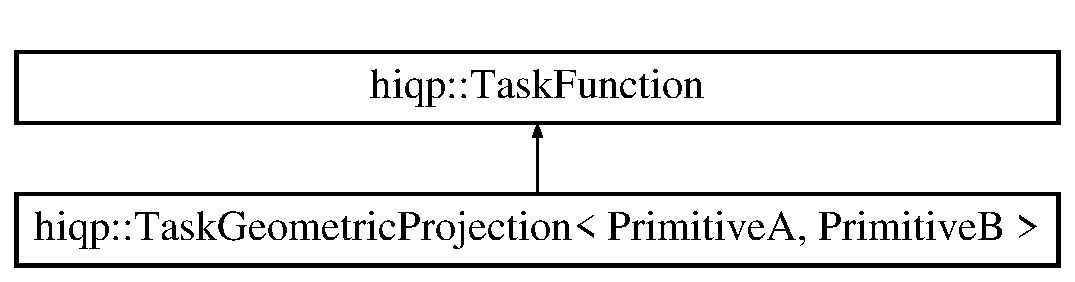
\includegraphics[height=2.000000cm]{classhiqp_1_1TaskGeometricProjection}
\end{center}
\end{figure}
\subsection*{Public Member Functions}
\begin{DoxyCompactItemize}
\item 
\hypertarget{classhiqp_1_1TaskGeometricProjection_af75d2b163680a57fc5809c9b07e3e678}{\hyperlink{classhiqp_1_1TaskGeometricProjection_af75d2b163680a57fc5809c9b07e3e678}{Task\-Geometric\-Projection} ()}\label{classhiqp_1_1TaskGeometricProjection_af75d2b163680a57fc5809c9b07e3e678}

\begin{DoxyCompactList}\small\item\em Constructor. \end{DoxyCompactList}\item 
\hypertarget{classhiqp_1_1TaskGeometricProjection_a53d6bb2b588b3667961ab97084dcd6ba}{\hyperlink{classhiqp_1_1TaskGeometricProjection_a53d6bb2b588b3667961ab97084dcd6ba}{$\sim$\-Task\-Geometric\-Projection} () noexcept}\label{classhiqp_1_1TaskGeometricProjection_a53d6bb2b588b3667961ab97084dcd6ba}

\begin{DoxyCompactList}\small\item\em Destructor. \end{DoxyCompactList}\item 
int \hyperlink{classhiqp_1_1TaskGeometricProjection_a40985179abed77a08e2ff35ce3bd714d}{init} (const \hyperlink{classhiqp_1_1HiQPTimePoint}{Hi\-Q\-P\-Time\-Point} \&sampling\-\_\-time, const std\-::vector$<$ std\-::string $>$ \&parameters, const K\-D\-L\-::\-Tree \&kdl\-\_\-tree, unsigned int num\-\_\-controls)
\begin{DoxyCompactList}\small\item\em Initializes the task. \end{DoxyCompactList}\item 
int \hyperlink{classhiqp_1_1TaskGeometricProjection_a3eaed2bb6db4b6b6b53503a20d2a1895}{apply} (const \hyperlink{classhiqp_1_1HiQPTimePoint}{Hi\-Q\-P\-Time\-Point} \&sampling\-\_\-time, const K\-D\-L\-::\-Tree \&kdl\-\_\-tree, const K\-D\-L\-::\-Jnt\-Array\-Vel \&kdl\-\_\-joint\-\_\-pos\-\_\-vel)
\begin{DoxyCompactList}\small\item\em Calculates the task function and task jacobian values. \end{DoxyCompactList}\item 
int \hyperlink{classhiqp_1_1TaskGeometricProjection_a6e824a39011d6e5865e13dd956649a71}{monitor} ()
\begin{DoxyCompactList}\small\item\em Computes all performance measures used when monitoring this task. \end{DoxyCompactList}\end{DoxyCompactItemize}
\subsection*{Additional Inherited Members}


\subsection{Detailed Description}
\subsubsection*{template$<$typename Primitive\-A, typename Primitive\-B$>$class hiqp\-::\-Task\-Geometric\-Projection$<$ Primitive\-A, Primitive\-B $>$}

It's awesome! 

\subsection{Member Function Documentation}
\hypertarget{classhiqp_1_1TaskGeometricProjection_a3eaed2bb6db4b6b6b53503a20d2a1895}{\index{hiqp\-::\-Task\-Geometric\-Projection@{hiqp\-::\-Task\-Geometric\-Projection}!apply@{apply}}
\index{apply@{apply}!hiqp::TaskGeometricProjection@{hiqp\-::\-Task\-Geometric\-Projection}}
\subsubsection[{apply}]{\setlength{\rightskip}{0pt plus 5cm}template$<$typename Primitive\-A , typename Primitive\-B $>$ int {\bf hiqp\-::\-Task\-Geometric\-Projection}$<$ Primitive\-A, Primitive\-B $>$\-::apply (
\begin{DoxyParamCaption}
\item[{const {\bf Hi\-Q\-P\-Time\-Point} \&}]{sampling\-\_\-time, }
\item[{const K\-D\-L\-::\-Tree \&}]{kdl\-\_\-tree, }
\item[{const K\-D\-L\-::\-Jnt\-Array\-Vel \&}]{kdl\-\_\-joint\-\_\-pos\-\_\-vel}
\end{DoxyParamCaption}
)\hspace{0.3cm}{\ttfamily [virtual]}}}\label{classhiqp_1_1TaskGeometricProjection_a3eaed2bb6db4b6b6b53503a20d2a1895}


Calculates the task function and task jacobian values. 


\begin{DoxyParams}{Parameters}
{\em kdl\-\_\-tree} & \-: reference to the kinematic dynamic tree of the robot \\
\hline
{\em joints\-\_\-pos\-\_\-vel} & \-: reference to the current joint positions and velocities\\
\hline
\end{DoxyParams}
\begin{DoxyReturn}{Returns}
true if the calculation was successful 
\end{DoxyReturn}


Implements \hyperlink{classhiqp_1_1TaskFunction_a3c476e011c762b8a8f7470ec47f70a17}{hiqp\-::\-Task\-Function}.

\hypertarget{classhiqp_1_1TaskGeometricProjection_a40985179abed77a08e2ff35ce3bd714d}{\index{hiqp\-::\-Task\-Geometric\-Projection@{hiqp\-::\-Task\-Geometric\-Projection}!init@{init}}
\index{init@{init}!hiqp::TaskGeometricProjection@{hiqp\-::\-Task\-Geometric\-Projection}}
\subsubsection[{init}]{\setlength{\rightskip}{0pt plus 5cm}template$<$typename Primitive\-A , typename Primitive\-B $>$ int {\bf hiqp\-::\-Task\-Geometric\-Projection}$<$ Primitive\-A, Primitive\-B $>$\-::init (
\begin{DoxyParamCaption}
\item[{const {\bf Hi\-Q\-P\-Time\-Point} \&}]{sampling\-\_\-time, }
\item[{const std\-::vector$<$ std\-::string $>$ \&}]{parameters, }
\item[{const K\-D\-L\-::\-Tree \&}]{kdl\-\_\-tree, }
\item[{unsigned int}]{num\-\_\-controls}
\end{DoxyParamCaption}
)\hspace{0.3cm}{\ttfamily [virtual]}}}\label{classhiqp_1_1TaskGeometricProjection_a40985179abed77a08e2ff35ce3bd714d}


Initializes the task. 

\begin{DoxyReturn}{Returns}
0 upon success 
\end{DoxyReturn}


Implements \hyperlink{classhiqp_1_1TaskFunction}{hiqp\-::\-Task\-Function}.

\hypertarget{classhiqp_1_1TaskGeometricProjection_a6e824a39011d6e5865e13dd956649a71}{\index{hiqp\-::\-Task\-Geometric\-Projection@{hiqp\-::\-Task\-Geometric\-Projection}!monitor@{monitor}}
\index{monitor@{monitor}!hiqp::TaskGeometricProjection@{hiqp\-::\-Task\-Geometric\-Projection}}
\subsubsection[{monitor}]{\setlength{\rightskip}{0pt plus 5cm}template$<$typename Primitive\-A , typename Primitive\-B $>$ int {\bf hiqp\-::\-Task\-Geometric\-Projection}$<$ Primitive\-A, Primitive\-B $>$\-::monitor (
\begin{DoxyParamCaption}
{}
\end{DoxyParamCaption}
)\hspace{0.3cm}{\ttfamily [virtual]}}}\label{classhiqp_1_1TaskGeometricProjection_a6e824a39011d6e5865e13dd956649a71}


Computes all performance measures used when monitoring this task. 

\begin{DoxyReturn}{Returns}
0 if the calculation was successful 
\end{DoxyReturn}


Implements \hyperlink{classhiqp_1_1TaskFunction_a47a3283a0c0ebafa17feeca96afe5af0}{hiqp\-::\-Task\-Function}.



The documentation for this class was generated from the following files\-:\begin{DoxyCompactItemize}
\item 
include/hiqp/tasks/\hyperlink{task__geometric__projection_8h}{task\-\_\-geometric\-\_\-projection.\-h}\item 
include/hiqp/tasks/\hyperlink{task__geometric__projection____impl_8h}{task\-\_\-geometric\-\_\-projection\-\_\-\-\_\-impl.\-h}\end{DoxyCompactItemize}

\hypertarget{classhiqp_1_1TaskJntConfig}{\section{hiqp\-:\-:Task\-Jnt\-Config Class Reference}
\label{classhiqp_1_1TaskJntConfig}\index{hiqp\-::\-Task\-Jnt\-Config@{hiqp\-::\-Task\-Jnt\-Config}}
}


Represents a task that sets a specific joint configuration.  




{\ttfamily \#include $<$task\-\_\-jnt\-\_\-config.\-h$>$}

Inheritance diagram for hiqp\-:\-:Task\-Jnt\-Config\-:\begin{figure}[H]
\begin{center}
\leavevmode
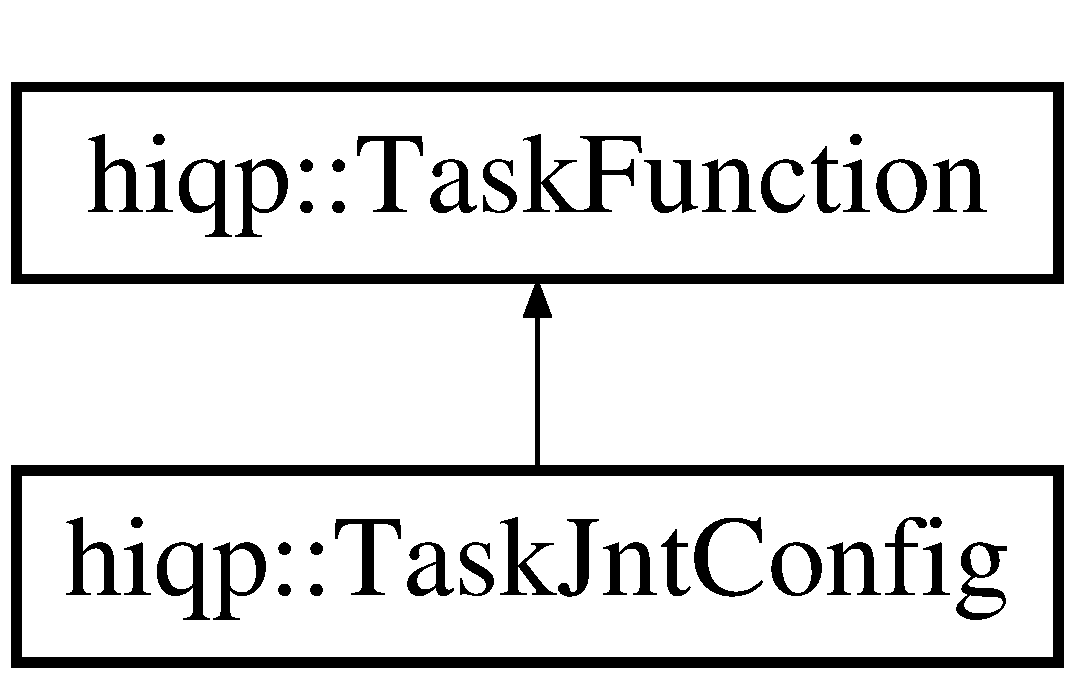
\includegraphics[height=2.000000cm]{classhiqp_1_1TaskJntConfig}
\end{center}
\end{figure}
\subsection*{Public Member Functions}
\begin{DoxyCompactItemize}
\item 
\hypertarget{classhiqp_1_1TaskJntConfig_a29b4fbc6207f5de40f3e880274f6f716}{\hyperlink{classhiqp_1_1TaskJntConfig_a29b4fbc6207f5de40f3e880274f6f716}{Task\-Jnt\-Config} ()}\label{classhiqp_1_1TaskJntConfig_a29b4fbc6207f5de40f3e880274f6f716}

\begin{DoxyCompactList}\small\item\em Constructor Constructs my awesome task. \end{DoxyCompactList}\item 
\hypertarget{classhiqp_1_1TaskJntConfig_aae049672adb68630748475005fe49ff4}{\hyperlink{classhiqp_1_1TaskJntConfig_aae049672adb68630748475005fe49ff4}{$\sim$\-Task\-Jnt\-Config} () noexcept}\label{classhiqp_1_1TaskJntConfig_aae049672adb68630748475005fe49ff4}

\begin{DoxyCompactList}\small\item\em Destructor Destructs my awesome task. \end{DoxyCompactList}\item 
int \hyperlink{classhiqp_1_1TaskJntConfig_a03d9d877da64b956d7afd91e536c7fcd}{init} (const \hyperlink{classhiqp_1_1HiQPTimePoint}{Hi\-Q\-P\-Time\-Point} \&sampling\-\_\-time, const std\-::vector$<$ std\-::string $>$ \&parameters, const K\-D\-L\-::\-Tree \&kdl\-\_\-tree, unsigned int num\-\_\-controls)
\begin{DoxyCompactList}\small\item\em {\itshape Pure virtual}. Initializes the task \end{DoxyCompactList}\item 
int \hyperlink{classhiqp_1_1TaskJntConfig_a34dd3b5a79953fa6c0f970dcdd66873b}{apply} (const \hyperlink{classhiqp_1_1HiQPTimePoint}{Hi\-Q\-P\-Time\-Point} \&sampling\-\_\-time, const K\-D\-L\-::\-Tree \&kdl\-\_\-tree, const K\-D\-L\-::\-Jnt\-Array\-Vel \&kdl\-\_\-joint\-\_\-pos\-\_\-vel)
\begin{DoxyCompactList}\small\item\em {\itshape Pure virtual}. Calculates the task function and task jacobian values. \end{DoxyCompactList}\item 
int \hyperlink{classhiqp_1_1TaskJntConfig_af4d673c3b78a3c461abce090c0871a63}{monitor} ()
\begin{DoxyCompactList}\small\item\em Computes all performance measures used when monitoring this task. \end{DoxyCompactList}\end{DoxyCompactItemize}
\subsection*{Additional Inherited Members}


\subsection{Detailed Description}
Represents a task that sets a specific joint configuration. 

This task does not leave any redundancy available to other tasks. 

\subsection{Member Function Documentation}
\hypertarget{classhiqp_1_1TaskJntConfig_a34dd3b5a79953fa6c0f970dcdd66873b}{\index{hiqp\-::\-Task\-Jnt\-Config@{hiqp\-::\-Task\-Jnt\-Config}!apply@{apply}}
\index{apply@{apply}!hiqp::TaskJntConfig@{hiqp\-::\-Task\-Jnt\-Config}}
\subsubsection[{apply}]{\setlength{\rightskip}{0pt plus 5cm}int hiqp\-::\-Task\-Jnt\-Config\-::apply (
\begin{DoxyParamCaption}
\item[{const {\bf Hi\-Q\-P\-Time\-Point} \&}]{sampling\-\_\-time, }
\item[{const K\-D\-L\-::\-Tree \&}]{kdl\-\_\-tree, }
\item[{const K\-D\-L\-::\-Jnt\-Array\-Vel \&}]{kdl\-\_\-joint\-\_\-pos\-\_\-vel}
\end{DoxyParamCaption}
)\hspace{0.3cm}{\ttfamily [virtual]}}}\label{classhiqp_1_1TaskJntConfig_a34dd3b5a79953fa6c0f970dcdd66873b}


{\itshape Pure virtual}. Calculates the task function and task jacobian values. 


\begin{DoxyParams}{Parameters}
{\em kdl\-\_\-tree} & \-: reference to the kinematic dynamic tree of the robot \\
\hline
{\em joints\-\_\-pos\-\_\-vel} & \-: reference to the current joint positions and velocities\\
\hline
\end{DoxyParams}
\begin{DoxyReturn}{Returns}
true if the calculation was successful 
\end{DoxyReturn}


Implements \hyperlink{classhiqp_1_1TaskFunction_a3c476e011c762b8a8f7470ec47f70a17}{hiqp\-::\-Task\-Function}.

\hypertarget{classhiqp_1_1TaskJntConfig_a03d9d877da64b956d7afd91e536c7fcd}{\index{hiqp\-::\-Task\-Jnt\-Config@{hiqp\-::\-Task\-Jnt\-Config}!init@{init}}
\index{init@{init}!hiqp::TaskJntConfig@{hiqp\-::\-Task\-Jnt\-Config}}
\subsubsection[{init}]{\setlength{\rightskip}{0pt plus 5cm}int hiqp\-::\-Task\-Jnt\-Config\-::init (
\begin{DoxyParamCaption}
\item[{const {\bf Hi\-Q\-P\-Time\-Point} \&}]{sampling\-\_\-time, }
\item[{const std\-::vector$<$ std\-::string $>$ \&}]{parameters, }
\item[{const K\-D\-L\-::\-Tree \&}]{kdl\-\_\-tree, }
\item[{unsigned int}]{num\-\_\-controls}
\end{DoxyParamCaption}
)\hspace{0.3cm}{\ttfamily [virtual]}}}\label{classhiqp_1_1TaskJntConfig_a03d9d877da64b956d7afd91e536c7fcd}


{\itshape Pure virtual}. Initializes the task 

\begin{DoxyReturn}{Returns}
0 upon success 
\end{DoxyReturn}


Implements \hyperlink{classhiqp_1_1TaskFunction}{hiqp\-::\-Task\-Function}.

\hypertarget{classhiqp_1_1TaskJntConfig_af4d673c3b78a3c461abce090c0871a63}{\index{hiqp\-::\-Task\-Jnt\-Config@{hiqp\-::\-Task\-Jnt\-Config}!monitor@{monitor}}
\index{monitor@{monitor}!hiqp::TaskJntConfig@{hiqp\-::\-Task\-Jnt\-Config}}
\subsubsection[{monitor}]{\setlength{\rightskip}{0pt plus 5cm}int hiqp\-::\-Task\-Jnt\-Config\-::monitor (
\begin{DoxyParamCaption}
{}
\end{DoxyParamCaption}
)\hspace{0.3cm}{\ttfamily [virtual]}}}\label{classhiqp_1_1TaskJntConfig_af4d673c3b78a3c461abce090c0871a63}


Computes all performance measures used when monitoring this task. 

\begin{DoxyReturn}{Returns}
0 if the calculation was successful 
\end{DoxyReturn}


Implements \hyperlink{classhiqp_1_1TaskFunction_a47a3283a0c0ebafa17feeca96afe5af0}{hiqp\-::\-Task\-Function}.



The documentation for this class was generated from the following files\-:\begin{DoxyCompactItemize}
\item 
include/hiqp/tasks/\hyperlink{task__jnt__config_8h}{task\-\_\-jnt\-\_\-config.\-h}\item 
src/tasks/\hyperlink{task__jnt__config_8cpp}{task\-\_\-jnt\-\_\-config.\-cpp}\end{DoxyCompactItemize}

\hypertarget{classTaskJntLimit}{\section{Task\-Jnt\-Limit Class Reference}
\label{classTaskJntLimit}\index{Task\-Jnt\-Limit@{Task\-Jnt\-Limit}}
}


Represents a task that limits joint velocities.  




{\ttfamily \#include $<$task\-\_\-jnt\-\_\-limits.\-h$>$}



\subsection{Detailed Description}
Represents a task that limits joint velocities. 

The documentation for this class was generated from the following file\-:\begin{DoxyCompactItemize}
\item 
include/hiqp/tasks/\hyperlink{task__jnt__limits_8h}{task\-\_\-jnt\-\_\-limits.\-h}\end{DoxyCompactItemize}

\hypertarget{classhiqp_1_1TaskJntLimits}{\section{hiqp\-:\-:Task\-Jnt\-Limits Class Reference}
\label{classhiqp_1_1TaskJntLimits}\index{hiqp\-::\-Task\-Jnt\-Limits@{hiqp\-::\-Task\-Jnt\-Limits}}
}
Inheritance diagram for hiqp\-:\-:Task\-Jnt\-Limits\-:\begin{figure}[H]
\begin{center}
\leavevmode
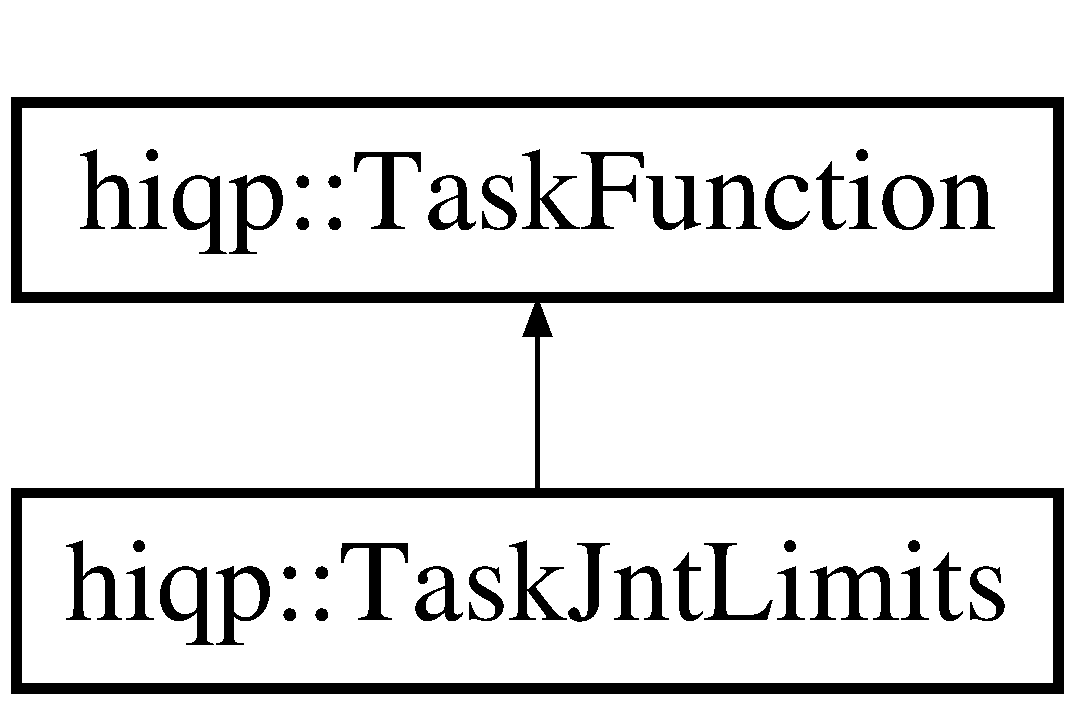
\includegraphics[height=2.000000cm]{classhiqp_1_1TaskJntLimits}
\end{center}
\end{figure}
\subsection*{Public Member Functions}
\begin{DoxyCompactItemize}
\item 
\hypertarget{classhiqp_1_1TaskJntLimits_a82d969e4fafcdd5a0830700ef1b67204}{\hyperlink{classhiqp_1_1TaskJntLimits_a82d969e4fafcdd5a0830700ef1b67204}{Task\-Jnt\-Limits} ()}\label{classhiqp_1_1TaskJntLimits_a82d969e4fafcdd5a0830700ef1b67204}

\begin{DoxyCompactList}\small\item\em Constructor Constructs my awesome task. \end{DoxyCompactList}\item 
\hypertarget{classhiqp_1_1TaskJntLimits_af6d3deb66428b31eada36154640134c0}{\hyperlink{classhiqp_1_1TaskJntLimits_af6d3deb66428b31eada36154640134c0}{$\sim$\-Task\-Jnt\-Limits} () noexcept}\label{classhiqp_1_1TaskJntLimits_af6d3deb66428b31eada36154640134c0}

\begin{DoxyCompactList}\small\item\em Destructor Destructs my awesome task. \end{DoxyCompactList}\item 
int \hyperlink{classhiqp_1_1TaskJntLimits_a9b5ae3ada59d143d57d8abd12c8e1e5f}{init} (const \hyperlink{classhiqp_1_1HiQPTimePoint}{Hi\-Q\-P\-Time\-Point} \&sampling\-\_\-time, const std\-::vector$<$ std\-::string $>$ \&parameters, const K\-D\-L\-::\-Tree \&kdl\-\_\-tree, unsigned int num\-\_\-controls)
\begin{DoxyCompactList}\small\item\em {\itshape Pure virtual}. Initializes the task \end{DoxyCompactList}\item 
int \hyperlink{classhiqp_1_1TaskJntLimits_aa140824f7bc5b80754f3b57b43d7aa69}{apply} (const \hyperlink{classhiqp_1_1HiQPTimePoint}{Hi\-Q\-P\-Time\-Point} \&sampling\-\_\-time, const K\-D\-L\-::\-Tree \&kdl\-\_\-tree, const K\-D\-L\-::\-Jnt\-Array\-Vel \&kdl\-\_\-joint\-\_\-pos\-\_\-vel)
\begin{DoxyCompactList}\small\item\em {\itshape Pure virtual}. Calculates the task function and task jacobian values. \end{DoxyCompactList}\item 
int \hyperlink{classhiqp_1_1TaskJntLimits_a1a2b92667aa173f74b2df4f1364ddcd9}{monitor} ()
\begin{DoxyCompactList}\small\item\em {\itshape Pure virtual}. Computes all performance measures used when monitoring this task. \end{DoxyCompactList}\end{DoxyCompactItemize}
\subsection*{Additional Inherited Members}


\subsection{Member Function Documentation}
\hypertarget{classhiqp_1_1TaskJntLimits_aa140824f7bc5b80754f3b57b43d7aa69}{\index{hiqp\-::\-Task\-Jnt\-Limits@{hiqp\-::\-Task\-Jnt\-Limits}!apply@{apply}}
\index{apply@{apply}!hiqp::TaskJntLimits@{hiqp\-::\-Task\-Jnt\-Limits}}
\subsubsection[{apply}]{\setlength{\rightskip}{0pt plus 5cm}int hiqp\-::\-Task\-Jnt\-Limits\-::apply (
\begin{DoxyParamCaption}
\item[{const {\bf Hi\-Q\-P\-Time\-Point} \&}]{sampling\-\_\-time, }
\item[{const K\-D\-L\-::\-Tree \&}]{kdl\-\_\-tree, }
\item[{const K\-D\-L\-::\-Jnt\-Array\-Vel \&}]{kdl\-\_\-joint\-\_\-pos\-\_\-vel}
\end{DoxyParamCaption}
)\hspace{0.3cm}{\ttfamily [virtual]}}}\label{classhiqp_1_1TaskJntLimits_aa140824f7bc5b80754f3b57b43d7aa69}


{\itshape Pure virtual}. Calculates the task function and task jacobian values. 


\begin{DoxyParams}{Parameters}
{\em kdl\-\_\-tree} & \-: reference to the kinematic dynamic tree of the robot \\
\hline
{\em joints\-\_\-pos\-\_\-vel} & \-: reference to the current joint positions and velocities\\
\hline
\end{DoxyParams}
\begin{DoxyReturn}{Returns}
true if the calculation was successful 
\end{DoxyReturn}


Implements \hyperlink{classhiqp_1_1TaskFunction_a3c476e011c762b8a8f7470ec47f70a17}{hiqp\-::\-Task\-Function}.

\hypertarget{classhiqp_1_1TaskJntLimits_a9b5ae3ada59d143d57d8abd12c8e1e5f}{\index{hiqp\-::\-Task\-Jnt\-Limits@{hiqp\-::\-Task\-Jnt\-Limits}!init@{init}}
\index{init@{init}!hiqp::TaskJntLimits@{hiqp\-::\-Task\-Jnt\-Limits}}
\subsubsection[{init}]{\setlength{\rightskip}{0pt plus 5cm}int hiqp\-::\-Task\-Jnt\-Limits\-::init (
\begin{DoxyParamCaption}
\item[{const {\bf Hi\-Q\-P\-Time\-Point} \&}]{sampling\-\_\-time, }
\item[{const std\-::vector$<$ std\-::string $>$ \&}]{parameters, }
\item[{const K\-D\-L\-::\-Tree \&}]{kdl\-\_\-tree, }
\item[{unsigned int}]{num\-\_\-controls}
\end{DoxyParamCaption}
)\hspace{0.3cm}{\ttfamily [virtual]}}}\label{classhiqp_1_1TaskJntLimits_a9b5ae3ada59d143d57d8abd12c8e1e5f}


{\itshape Pure virtual}. Initializes the task 

\begin{DoxyReturn}{Returns}
0 upon success 
\end{DoxyReturn}


Implements \hyperlink{classhiqp_1_1TaskFunction}{hiqp\-::\-Task\-Function}.

\hypertarget{classhiqp_1_1TaskJntLimits_a1a2b92667aa173f74b2df4f1364ddcd9}{\index{hiqp\-::\-Task\-Jnt\-Limits@{hiqp\-::\-Task\-Jnt\-Limits}!monitor@{monitor}}
\index{monitor@{monitor}!hiqp::TaskJntLimits@{hiqp\-::\-Task\-Jnt\-Limits}}
\subsubsection[{monitor}]{\setlength{\rightskip}{0pt plus 5cm}int hiqp\-::\-Task\-Jnt\-Limits\-::monitor (
\begin{DoxyParamCaption}
{}
\end{DoxyParamCaption}
)\hspace{0.3cm}{\ttfamily [virtual]}}}\label{classhiqp_1_1TaskJntLimits_a1a2b92667aa173f74b2df4f1364ddcd9}


{\itshape Pure virtual}. Computes all performance measures used when monitoring this task. 

\begin{DoxyReturn}{Returns}
0 if the calculation was successful 
\end{DoxyReturn}


Implements \hyperlink{classhiqp_1_1TaskFunction_a47a3283a0c0ebafa17feeca96afe5af0}{hiqp\-::\-Task\-Function}.



The documentation for this class was generated from the following files\-:\begin{DoxyCompactItemize}
\item 
include/hiqp/tasks/\hyperlink{task__jnt__limits_8h}{task\-\_\-jnt\-\_\-limits.\-h}\item 
src/tasks/\hyperlink{task__jnt__limits_8cpp}{task\-\_\-jnt\-\_\-limits.\-cpp}\end{DoxyCompactItemize}

\hypertarget{classhiqp_1_1TaskManager}{\section{hiqp\-:\-:Task\-Manager Class Reference}
\label{classhiqp_1_1TaskManager}\index{hiqp\-::\-Task\-Manager@{hiqp\-::\-Task\-Manager}}
}


Should be created only once!  




{\ttfamily \#include $<$task\-\_\-manager.\-h$>$}

\subsection*{Public Member Functions}
\begin{DoxyCompactItemize}
\item 
\hypertarget{classhiqp_1_1TaskManager_af190d8f0b3ee1c0d32acdb70fae6e03d}{\hyperlink{classhiqp_1_1TaskManager_af190d8f0b3ee1c0d32acdb70fae6e03d}{Task\-Manager} ()}\label{classhiqp_1_1TaskManager_af190d8f0b3ee1c0d32acdb70fae6e03d}

\begin{DoxyCompactList}\small\item\em Constructor Constructs my awesome controller. \end{DoxyCompactList}\item 
\hypertarget{classhiqp_1_1TaskManager_a688ad548e2ef681b458c1fc90326f6e6}{\hyperlink{classhiqp_1_1TaskManager_a688ad548e2ef681b458c1fc90326f6e6}{$\sim$\-Task\-Manager} () noexcept}\label{classhiqp_1_1TaskManager_a688ad548e2ef681b458c1fc90326f6e6}

\begin{DoxyCompactList}\small\item\em Destructor Destructs my awesome manager. \end{DoxyCompactList}\item 
bool \hyperlink{classhiqp_1_1TaskManager_a9243435c3819b03a9874f47d985a2147}{get\-Kinematic\-Controls} (const K\-D\-L\-::\-Tree \&kdl\-\_\-tree, const K\-D\-L\-::\-Jnt\-Array\-Vel \&kdl\-\_\-joint\-\_\-pos\-\_\-vel, unsigned int n\-\_\-controls, std\-::vector$<$ double $>$ \&controls)
\begin{DoxyCompactList}\small\item\em Called every time the controller is initialized by the ros\-::controller\-\_\-manager. \end{DoxyCompactList}\end{DoxyCompactItemize}


\subsection{Detailed Description}
Should be created only once! 

It's awesome! 

\subsection{Member Function Documentation}
\hypertarget{classhiqp_1_1TaskManager_a9243435c3819b03a9874f47d985a2147}{\index{hiqp\-::\-Task\-Manager@{hiqp\-::\-Task\-Manager}!get\-Kinematic\-Controls@{get\-Kinematic\-Controls}}
\index{get\-Kinematic\-Controls@{get\-Kinematic\-Controls}!hiqp::TaskManager@{hiqp\-::\-Task\-Manager}}
\subsubsection[{get\-Kinematic\-Controls}]{\setlength{\rightskip}{0pt plus 5cm}bool hiqp\-::\-Task\-Manager\-::get\-Kinematic\-Controls (
\begin{DoxyParamCaption}
\item[{const K\-D\-L\-::\-Tree \&}]{kdl\-\_\-tree, }
\item[{const K\-D\-L\-::\-Jnt\-Array\-Vel \&}]{kdl\-\_\-joint\-\_\-pos\-\_\-vel, }
\item[{unsigned int}]{n\-\_\-controls, }
\item[{std\-::vector$<$ double $>$ \&}]{controls}
\end{DoxyParamCaption}
)}}\label{classhiqp_1_1TaskManager_a9243435c3819b03a9874f47d985a2147}


Called every time the controller is initialized by the ros\-::controller\-\_\-manager. 

Does some cool stuff!


\begin{DoxyParams}{Parameters}
{\em kdl\-\_\-tree} & \-: the kinematic dynamic tree of the robot \\
\hline
{\em n\-\_\-controls} & \-: the number of controls \\
\hline
{\em controls} & \-: reference to the controls data \\
\hline
\end{DoxyParams}
\begin{DoxyReturn}{Returns}
true if the initialization was successful 
\end{DoxyReturn}


The documentation for this class was generated from the following files\-:\begin{DoxyCompactItemize}
\item 
include/\hyperlink{task__manager_8h}{task\-\_\-manager.\-h}\item 
src/task\-\_\-manager.\-cpp\end{DoxyCompactItemize}

\hypertarget{classhiqp_1_1TaskMonitoringData}{\section{hiqp\-:\-:Task\-Monitoring\-Data Class Reference}
\label{classhiqp_1_1TaskMonitoringData}\index{hiqp\-::\-Task\-Monitoring\-Data@{hiqp\-::\-Task\-Monitoring\-Data}}
}


An aggregation of const references to facilitate communication of monitoring data.  




{\ttfamily \#include $<$task\-\_\-manager.\-h$>$}

\subsection*{Public Member Functions}
\begin{DoxyCompactItemize}
\item 
\hypertarget{classhiqp_1_1TaskMonitoringData_a33f6baf4d20a2ef1a7e89e4e7ea3ef7b}{{\bfseries Task\-Monitoring\-Data} (const std\-::string \&task\-\_\-name, const std\-::string \&measure\-\_\-tag, const std\-::vector$<$ double $>$ \&performance\-\_\-measures)}\label{classhiqp_1_1TaskMonitoringData_a33f6baf4d20a2ef1a7e89e4e7ea3ef7b}

\end{DoxyCompactItemize}
\subsection*{Public Attributes}
\begin{DoxyCompactItemize}
\item 
\hypertarget{classhiqp_1_1TaskMonitoringData_a51d485d0b298dd0e4859744cf33a8227}{const std\-::string \& {\bfseries task\-\_\-name\-\_\-}}\label{classhiqp_1_1TaskMonitoringData_a51d485d0b298dd0e4859744cf33a8227}

\item 
\hypertarget{classhiqp_1_1TaskMonitoringData_af27f6d903e69473949feb16e2e82cd69}{std\-::string {\bfseries measure\-\_\-tag\-\_\-}}\label{classhiqp_1_1TaskMonitoringData_af27f6d903e69473949feb16e2e82cd69}

\item 
\hypertarget{classhiqp_1_1TaskMonitoringData_a693c5b1df002e1558df125f268057e91}{const std\-::vector$<$ double $>$ \& {\bfseries performance\-\_\-measures\-\_\-}}\label{classhiqp_1_1TaskMonitoringData_a693c5b1df002e1558df125f268057e91}

\end{DoxyCompactItemize}


\subsection{Detailed Description}
An aggregation of const references to facilitate communication of monitoring data. 

The documentation for this class was generated from the following file\-:\begin{DoxyCompactItemize}
\item 
include/hiqp/task\-\_\-manager.\-h\end{DoxyCompactItemize}

\hypertarget{classhiqp_1_1Visualizer}{\section{hiqp\-:\-:Visualizer Class Reference}
\label{classhiqp_1_1Visualizer}\index{hiqp\-::\-Visualizer@{hiqp\-::\-Visualizer}}
}
Inheritance diagram for hiqp\-:\-:Visualizer\-:\begin{figure}[H]
\begin{center}
\leavevmode
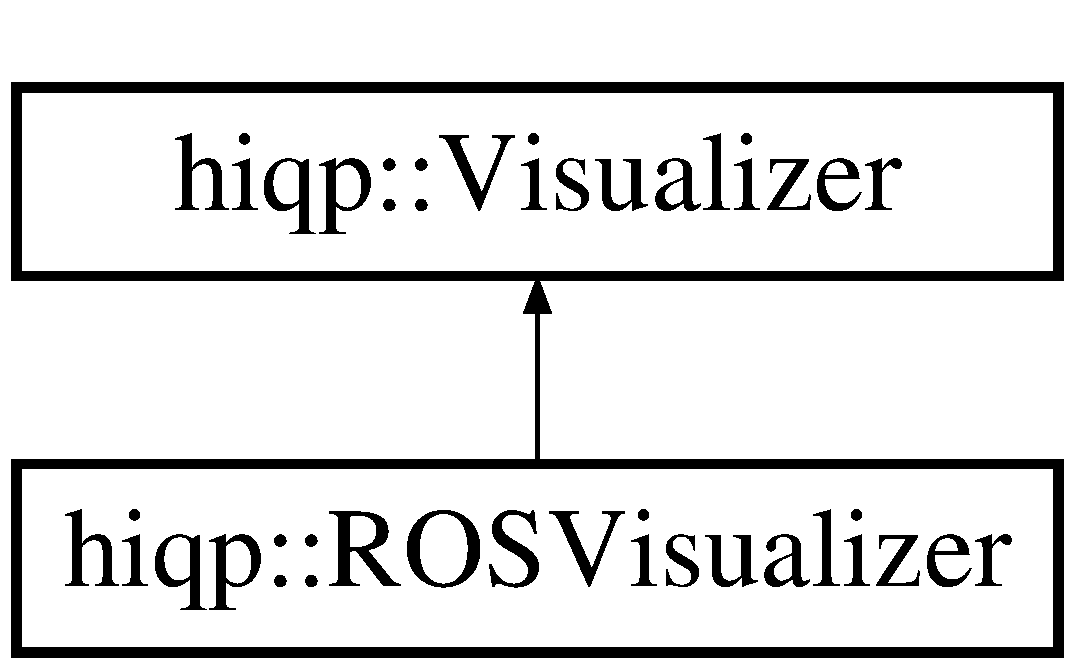
\includegraphics[height=2.000000cm]{classhiqp_1_1Visualizer}
\end{center}
\end{figure}
\subsection*{Public Member Functions}
\begin{DoxyCompactItemize}
\item 
\hypertarget{classhiqp_1_1Visualizer_a3408ea152dad3f1e84ea10f6dcf1ddfa}{virtual int {\bfseries add} (Geometric\-Point $\ast$point)=0}\label{classhiqp_1_1Visualizer_a3408ea152dad3f1e84ea10f6dcf1ddfa}

\item 
\hypertarget{classhiqp_1_1Visualizer_a006996d7fe4fa5da95f5fe8a5ffe4b49}{virtual int {\bfseries add} (Geometric\-Line $\ast$line)=0}\label{classhiqp_1_1Visualizer_a006996d7fe4fa5da95f5fe8a5ffe4b49}

\item 
\hypertarget{classhiqp_1_1Visualizer_ab04339fd46f98e6dac9786437bbd453e}{virtual int {\bfseries add} (Geometric\-Plane $\ast$plane)=0}\label{classhiqp_1_1Visualizer_ab04339fd46f98e6dac9786437bbd453e}

\item 
\hypertarget{classhiqp_1_1Visualizer_ada64cd2f429aa3da7b5efde5a74c5032}{virtual int {\bfseries add} (Geometric\-Box $\ast$box)=0}\label{classhiqp_1_1Visualizer_ada64cd2f429aa3da7b5efde5a74c5032}

\item 
\hypertarget{classhiqp_1_1Visualizer_af50a44f684fe1d56401489715f555ed6}{virtual int {\bfseries add} (Geometric\-Cylinder $\ast$cylinder)=0}\label{classhiqp_1_1Visualizer_af50a44f684fe1d56401489715f555ed6}

\item 
\hypertarget{classhiqp_1_1Visualizer_ab4f23d245fbd7b525bedaf4b94ea4d66}{virtual int {\bfseries add} (Geometric\-Sphere $\ast$sphere)=0}\label{classhiqp_1_1Visualizer_ab4f23d245fbd7b525bedaf4b94ea4d66}

\item 
\hypertarget{classhiqp_1_1Visualizer_a0cc4b3f0e99fc3ece0f895ae83ed272a}{virtual void {\bfseries update} (int id, Geometric\-Point $\ast$point)=0}\label{classhiqp_1_1Visualizer_a0cc4b3f0e99fc3ece0f895ae83ed272a}

\item 
\hypertarget{classhiqp_1_1Visualizer_ab4b295c193b298306b6746cd2be28f77}{virtual void {\bfseries update} (int id, Geometric\-Line $\ast$line)=0}\label{classhiqp_1_1Visualizer_ab4b295c193b298306b6746cd2be28f77}

\item 
\hypertarget{classhiqp_1_1Visualizer_aad1fd45a3e14dbabe58778a8697022b6}{virtual void {\bfseries update} (int id, Geometric\-Plane $\ast$plane)=0}\label{classhiqp_1_1Visualizer_aad1fd45a3e14dbabe58778a8697022b6}

\item 
\hypertarget{classhiqp_1_1Visualizer_a204181a69bc76206e29900087f7b15d3}{virtual void {\bfseries update} (int id, Geometric\-Box $\ast$box)=0}\label{classhiqp_1_1Visualizer_a204181a69bc76206e29900087f7b15d3}

\item 
\hypertarget{classhiqp_1_1Visualizer_a5f77dc4be5a52e37a52a261e173e2d74}{virtual void {\bfseries update} (int id, Geometric\-Cylinder $\ast$cylinder)=0}\label{classhiqp_1_1Visualizer_a5f77dc4be5a52e37a52a261e173e2d74}

\item 
\hypertarget{classhiqp_1_1Visualizer_a261eb1f1a838c7b1d536cb5ae14b0fd1}{virtual void {\bfseries update} (int id, Geometric\-Sphere $\ast$sphere)=0}\label{classhiqp_1_1Visualizer_a261eb1f1a838c7b1d536cb5ae14b0fd1}

\item 
\hypertarget{classhiqp_1_1Visualizer_a1128e99c71c44daefb4086316347928e}{virtual void {\bfseries remove} (int id)=0}\label{classhiqp_1_1Visualizer_a1128e99c71c44daefb4086316347928e}

\item 
\hypertarget{classhiqp_1_1Visualizer_a0e6cbf0da4f9e223ce676cff9d5de8ef}{virtual void {\bfseries remove\-Many} (const std\-::vector$<$ int $>$ \&ids)=0}\label{classhiqp_1_1Visualizer_a0e6cbf0da4f9e223ce676cff9d5de8ef}

\end{DoxyCompactItemize}


The documentation for this class was generated from the following file\-:\begin{DoxyCompactItemize}
\item 
include/hiqp/\hyperlink{visualizer_8h}{visualizer.\-h}\end{DoxyCompactItemize}

\chapter{File Documentation}
\hypertarget{hiqp__solver_8h}{\section{include/hiqp/hiqp\-\_\-solver.h File Reference}
\label{hiqp__solver_8h}\index{include/hiqp/hiqp\-\_\-solver.\-h@{include/hiqp/hiqp\-\_\-solver.\-h}}
}


Brief description of file.  


{\ttfamily \#include $<$map$>$}\\*
{\ttfamily \#include $<$vector$>$}\\*
{\ttfamily \#include $<$iostream$>$}\\*
{\ttfamily \#include $<$Eigen/\-Dense$>$}\\*
\subsection*{Classes}
\begin{DoxyCompactItemize}
\item 
struct \hyperlink{structhiqp_1_1HiQPStage}{hiqp\-::\-Hi\-Q\-P\-Stage}
\item 
class \hyperlink{classhiqp_1_1HiQPSolver}{hiqp\-::\-Hi\-Q\-P\-Solver}
\end{DoxyCompactItemize}
\subsection*{Namespaces}
\begin{DoxyCompactItemize}
\item 
\hyperlink{namespacehiqp}{hiqp}
\end{DoxyCompactItemize}


\subsection{Detailed Description}
Brief description of file. Marcus A Johansson (\href{mailto:marcus.adam.johansson@gmail.com}{\tt marcus.\-adam.\-johansson@gmail.\-com}) \begin{DoxyDate}{Date}
July, 2016 Detailed description of file. 
\end{DoxyDate}

\hypertarget{hiqp__time__point_8h}{\section{include/hiqp/hiqp\-\_\-time\-\_\-point.h File Reference}
\label{hiqp__time__point_8h}\index{include/hiqp/hiqp\-\_\-time\-\_\-point.\-h@{include/hiqp/hiqp\-\_\-time\-\_\-point.\-h}}
}


Brief description of file.  


\subsection*{Classes}
\begin{DoxyCompactItemize}
\item 
class \hyperlink{classhiqp_1_1HiQPTimePoint}{hiqp\-::\-Hi\-Q\-P\-Time\-Point}
\begin{DoxyCompactList}\small\item\em The time type used in this framework. \end{DoxyCompactList}\end{DoxyCompactItemize}
\subsection*{Namespaces}
\begin{DoxyCompactItemize}
\item 
\hyperlink{namespacehiqp}{hiqp}
\end{DoxyCompactItemize}


\subsection{Detailed Description}
Brief description of file. \begin{DoxyAuthor}{Author}
Marcus A Johansson (\href{mailto:marcus.adam.johansson@gmail.com}{\tt marcus.\-adam.\-johansson@gmail.\-com}) 
\end{DoxyAuthor}
\begin{DoxyDate}{Date}
July, 2016 Detailed description of file. 
\end{DoxyDate}

\hypertarget{hiqp__utils_8h}{\section{include/hiqp/hiqp\-\_\-utils.h File Reference}
\label{hiqp__utils_8h}\index{include/hiqp/hiqp\-\_\-utils.\-h@{include/hiqp/hiqp\-\_\-utils.\-h}}
}


Brief description of file.  


{\ttfamily \#include $<$iostream$>$}\\*
{\ttfamily \#include $<$kdl/frames.\-hpp$>$}\\*
{\ttfamily \#include $<$kdl/tree.\-hpp$>$}\\*
{\ttfamily \#include $<$kdl/framevel.\-hpp$>$}\\*
{\ttfamily \#include $<$kdl/jntarray.\-hpp$>$}\\*
{\ttfamily \#include $<$kdl/jntarrayvel.\-hpp$>$}\\*
{\ttfamily \#include $<$kdl/jacobian.\-hpp$>$}\\*
{\ttfamily \#include $<$Eigen/\-Dense$>$}\\*
\subsection*{Functions}
\begin{DoxyCompactItemize}
\item 
\hypertarget{namespacehiqp_ae25bb9b7205ab2630606197e8a35af8f}{std\-::ostream \& {\bfseries hiqp\-::operator$<$$<$} (std\-::ostream \&os, const K\-D\-L\-::\-Vector \&kdl\-\_\-vector)}\label{namespacehiqp_ae25bb9b7205ab2630606197e8a35af8f}

\item 
\hypertarget{namespacehiqp_ace17cd6f24f52ba09f129ab50f435f99}{std\-::ostream \& {\bfseries hiqp\-::operator$<$$<$} (std\-::ostream \&os, const K\-D\-L\-::\-Tree \&kdl\-\_\-tree)}\label{namespacehiqp_ace17cd6f24f52ba09f129ab50f435f99}

\item 
\hypertarget{namespacehiqp_a59fe109d0df644e9ead2b56f8d86bf89}{std\-::ostream \& {\bfseries hiqp\-::operator$<$$<$} (std\-::ostream \&os, const K\-D\-L\-::\-Frame\-Vel \&kdl\-\_\-frame\-\_\-vel)}\label{namespacehiqp_a59fe109d0df644e9ead2b56f8d86bf89}

\item 
\hypertarget{namespacehiqp_a33d4a297971bc3e2996aa1f3194b0e30}{std\-::ostream \& {\bfseries hiqp\-::operator$<$$<$} (std\-::ostream \&os, const K\-D\-L\-::\-Jnt\-Array\-Vel \&kdl\-\_\-joints\-\_\-vel)}\label{namespacehiqp_a33d4a297971bc3e2996aa1f3194b0e30}

\item 
\hypertarget{namespacehiqp_a6a26da69453463527d0b4c99884983c9}{std\-::ostream \& {\bfseries hiqp\-::operator$<$$<$} (std\-::ostream \&os, const K\-D\-L\-::\-Chain \&kdl\-\_\-chain)}\label{namespacehiqp_a6a26da69453463527d0b4c99884983c9}

\item 
\hypertarget{namespacehiqp_a95f3af7af45e7c81eda13572f2d3cc38}{int {\bfseries hiqp\-::kdl\-\_\-get\-Q\-Nr\-From\-Joint\-Name} (const K\-D\-L\-::\-Tree \&kdl\-\_\-tree, const std\-::string \&joint\-\_\-name)}\label{namespacehiqp_a95f3af7af45e7c81eda13572f2d3cc38}

\item 
\hypertarget{namespacehiqp_afc65617e444dcefe5ca39e0dac2a17b2}{int {\bfseries hiqp\-::kdl\-\_\-get\-Q\-Nr\-From\-Link\-Name} (const K\-D\-L\-::\-Tree \&kdl\-\_\-tree, const std\-::string \&link\-\_\-name)}\label{namespacehiqp_afc65617e444dcefe5ca39e0dac2a17b2}

\item 
\hypertarget{namespacehiqp_a9266d35577397a64d24935da167b406a}{int {\bfseries hiqp\-::kdl\-\_\-\-Jnt\-To\-Jac} (const K\-D\-L\-::\-Tree \&tree, const K\-D\-L\-::\-Jnt\-Array\-Vel \&qqdot, K\-D\-L\-::\-Jacobian \&jac, const std\-::string \&segmentname)}\label{namespacehiqp_a9266d35577397a64d24935da167b406a}

\item 
\hypertarget{namespacehiqp_aed9588cb786450e506ca68402880b1d8}{void {\bfseries hiqp\-::print\-Hiqp\-Info} (const std\-::string \&msg)}\label{namespacehiqp_aed9588cb786450e506ca68402880b1d8}

\item 
\hypertarget{namespacehiqp_a0993b019bfc0f0e2b38e76b2979eb0e0}{void {\bfseries hiqp\-::print\-Hiqp\-Warning} (const std\-::string \&msg)}\label{namespacehiqp_a0993b019bfc0f0e2b38e76b2979eb0e0}

\item 
{\footnotesize template$<$typename Derived $>$ }\\Derived {\bfseries hiqp\-::pinv} (const Eigen\-::\-Matrix\-Base$<$ Derived $>$ \&a)
\begin{DoxyCompactList}\small\item\em calculates the Moore-\/\-Penrose Pseudoinverse for any sized matrices. \end{DoxyCompactList}\item 
{\footnotesize template$<$typename Derived $>$ }\\Derived {\bfseries hiqp\-::dls} (const Eigen\-::\-Matrix\-Base$<$ Derived $>$ \&a, double eta=0.\-01)
\begin{DoxyCompactList}\small\item\em calculates the Damped-\/\-Least-\/\-Square matrix. \end{DoxyCompactList}\end{DoxyCompactItemize}


\subsection{Detailed Description}
Brief description of file. Marcus A Johansson (\href{mailto:marcus.adam.johansson@gmail.com}{\tt marcus.\-adam.\-johansson@gmail.\-com}) \begin{DoxyDate}{Date}
July, 2016 Detailed description of file. 
\end{DoxyDate}

\hypertarget{ros__kinematics__controller_8h}{\section{include/hiqp/ros\-\_\-kinematics\-\_\-controller.h File Reference}
\label{ros__kinematics__controller_8h}\index{include/hiqp/ros\-\_\-kinematics\-\_\-controller.\-h@{include/hiqp/ros\-\_\-kinematics\-\_\-controller.\-h}}
}


Brief description of file.  


{\ttfamily \#include $<$string$>$}\\*
{\ttfamily \#include $<$vector$>$}\\*
{\ttfamily \#include $<$mutex$>$}\\*
{\ttfamily \#include $<$ros/ros.\-h$>$}\\*
{\ttfamily \#include $<$ros/node\-\_\-handle.\-h$>$}\\*
{\ttfamily \#include $<$controller\-\_\-interface/controller.\-h$>$}\\*
{\ttfamily \#include $<$hardware\-\_\-interface/joint\-\_\-command\-\_\-interface.\-h$>$}\\*
{\ttfamily \#include $<$kdl/tree.\-hpp$>$}\\*
{\ttfamily \#include $<$kdl/jntarray.\-hpp$>$}\\*
{\ttfamily \#include $<$kdl/jntarrayvel.\-hpp$>$}\\*
{\ttfamily \#include $<$kdl\-\_\-parser/kdl\-\_\-parser.\-hpp$>$}\\*
{\ttfamily \#include $<$hiqp/task\-\_\-manager.\-h$>$}\\*
{\ttfamily \#include $<$hiqp/ros\-\_\-visualizer.\-h$>$}\\*
{\ttfamily \#include $<$hiqp/ros\-\_\-topic\-\_\-subscriber.\-h$>$}\\*
{\ttfamily \#include $<$hiqp/hiqp\-\_\-time\-\_\-point.\-h$>$}\\*
{\ttfamily \#include $<$hiqp\-\_\-msgs\-\_\-srvs/\-Add\-Task.\-h$>$}\\*
{\ttfamily \#include $<$hiqp\-\_\-msgs\-\_\-srvs/\-Update\-Task.\-h$>$}\\*
{\ttfamily \#include $<$hiqp\-\_\-msgs\-\_\-srvs/\-Remove\-Task.\-h$>$}\\*
{\ttfamily \#include $<$hiqp\-\_\-msgs\-\_\-srvs/\-Remove\-All\-Tasks.\-h$>$}\\*
{\ttfamily \#include $<$hiqp\-\_\-msgs\-\_\-srvs/\-Add\-Geometric\-Primitive.\-h$>$}\\*
{\ttfamily \#include $<$hiqp\-\_\-msgs\-\_\-srvs/\-Remove\-Geometric\-Primitive.\-h$>$}\\*
{\ttfamily \#include $<$hiqp\-\_\-msgs\-\_\-srvs/\-Remove\-All\-Geometric\-Primitives.\-h$>$}\\*
\subsection*{Classes}
\begin{DoxyCompactItemize}
\item 
class \hyperlink{classhiqp_1_1ROSKinematicsController}{hiqp\-::\-R\-O\-S\-Kinematics\-Controller}
\end{DoxyCompactItemize}
\subsection*{Namespaces}
\begin{DoxyCompactItemize}
\item 
\hyperlink{namespacehiqp}{hiqp}
\end{DoxyCompactItemize}
\subsection*{Typedefs}
\begin{DoxyCompactItemize}
\item 
typedef \\*
controller\-\_\-interface\-::\-Controller\\*
$<$ hardware\-\_\-interface\-::\-Velocity\-Joint\-Interface $>$ \hyperlink{namespacehiqp_a7b250295f6797153486ce8ab085bd450}{hiqp\-::\-Joint\-Velocity\-Controller}
\item 
typedef \\*
hardware\-\_\-interface\-::\-Velocity\-Joint\-Interface \hyperlink{namespacehiqp_ac536ca3b4ba33489281fa5bec490799c}{hiqp\-::\-Joint\-Velocity\-Interface}
\end{DoxyCompactItemize}


\subsection{Detailed Description}
Brief description of file. Marcus A Johansson (\href{mailto:marcus.adam.johansson@gmail.com}{\tt marcus.\-adam.\-johansson@gmail.\-com}) \begin{DoxyDate}{Date}
July, 2016 Detailed description of file. 
\end{DoxyDate}

\hypertarget{ros__visualizer_8h}{\section{include/hiqp/ros\-\_\-visualizer.h File Reference}
\label{ros__visualizer_8h}\index{include/hiqp/ros\-\_\-visualizer.\-h@{include/hiqp/ros\-\_\-visualizer.\-h}}
}


Brief description of file.  


{\ttfamily \#include $<$hiqp/visualizer.\-h$>$}\\*
{\ttfamily \#include $<$ros/ros.\-h$>$}\\*
\subsection*{Classes}
\begin{DoxyCompactItemize}
\item 
class \hyperlink{classhiqp_1_1ROSVisualizer}{hiqp\-::\-R\-O\-S\-Visualizer}
\end{DoxyCompactItemize}


\subsection{Detailed Description}
Brief description of file. Marcus A Johansson (\href{mailto:marcus.adam.johansson@gmail.com}{\tt marcus.\-adam.\-johansson@gmail.\-com}) \begin{DoxyDate}{Date}
July, 2016 Detailed description of file. 
\end{DoxyDate}

\hypertarget{casadi__solver_8h}{\section{include/hiqp/solvers/casadi\-\_\-solver.h File Reference}
\label{casadi__solver_8h}\index{include/hiqp/solvers/casadi\-\_\-solver.\-h@{include/hiqp/solvers/casadi\-\_\-solver.\-h}}
}


Brief description of file.  


{\ttfamily \#include $<$hiqp/hiqp\-\_\-solver.\-h$>$}\\*
\subsection*{Classes}
\begin{DoxyCompactItemize}
\item 
class \hyperlink{classhiqp_1_1CasADiSolver}{hiqp\-::\-Cas\-A\-Di\-Solver}
\end{DoxyCompactItemize}
\subsection*{Namespaces}
\begin{DoxyCompactItemize}
\item 
\hyperlink{namespacehiqp}{hiqp}
\end{DoxyCompactItemize}


\subsection{Detailed Description}
Brief description of file. Marcus A Johansson (\href{mailto:marcus.adam.johansson@gmail.com}{\tt marcus.\-adam.\-johansson@gmail.\-com}) \begin{DoxyDate}{Date}
July, 2016 Detailed description of file. 
\end{DoxyDate}

\hypertarget{task__dynamics_8h}{\section{include/hiqp/task\-\_\-dynamics.h File Reference}
\label{task__dynamics_8h}\index{include/hiqp/task\-\_\-dynamics.\-h@{include/hiqp/task\-\_\-dynamics.\-h}}
}


Brief description of file.  


{\ttfamily \#include $<$hiqp/hiqp\-\_\-time\-\_\-point.\-h$>$}\\*
{\ttfamily \#include $<$vector$>$}\\*
{\ttfamily \#include $<$chrono$>$}\\*
{\ttfamily \#include $<$Eigen/\-Dense$>$}\\*
\subsection*{Classes}
\begin{DoxyCompactItemize}
\item 
class \hyperlink{classhiqp_1_1TaskDynamics}{hiqp\-::\-Task\-Dynamics}
\begin{DoxyCompactList}\small\item\em Abstract base class for all task dynamics types. \end{DoxyCompactList}\end{DoxyCompactItemize}


\subsection{Detailed Description}
Brief description of file. Marcus A Johansson (\href{mailto:marcus.adam.johansson@gmail.com}{\tt marcus.\-adam.\-johansson@gmail.\-com}) \begin{DoxyDate}{Date}
July, 2016 Detailed description of file. 
\end{DoxyDate}

\hypertarget{task__function_8h}{\section{include/hiqp/task\-\_\-function.h File Reference}
\label{task__function_8h}\index{include/hiqp/task\-\_\-function.\-h@{include/hiqp/task\-\_\-function.\-h}}
}


Brief description of file.  


{\ttfamily \#include $<$hiqp/task\-\_\-dynamics.\-h$>$}\\*
{\ttfamily \#include $<$hiqp/visualizer.\-h$>$}\\*
{\ttfamily \#include $<$hiqp/hiqp\-\_\-time\-\_\-point.\-h$>$}\\*
{\ttfamily \#include $<$hiqp/geometric\-\_\-primitives/geometric\-\_\-primitive\-\_\-map.\-h$>$}\\*
{\ttfamily \#include $<$vector$>$}\\*
{\ttfamily \#include $<$iostream$>$}\\*
{\ttfamily \#include $<$chrono$>$}\\*
{\ttfamily \#include $<$Eigen/\-Dense$>$}\\*
{\ttfamily \#include $<$kdl/tree.\-hpp$>$}\\*
{\ttfamily \#include $<$kdl/jntarrayvel.\-hpp$>$}\\*
\subsection*{Classes}
\begin{DoxyCompactItemize}
\item 
class \hyperlink{classhiqp_1_1TaskFunction}{hiqp\-::\-Task\-Function}
\end{DoxyCompactItemize}
\subsection*{Namespaces}
\begin{DoxyCompactItemize}
\item 
\hyperlink{namespacehiqp}{hiqp}
\end{DoxyCompactItemize}


\subsection{Detailed Description}
Brief description of file. Marcus A Johansson (\href{mailto:marcus.adam.johansson@gmail.com}{\tt marcus.\-adam.\-johansson@gmail.\-com}) \begin{DoxyDate}{Date}
July, 2016 Detailed description of file. 
\end{DoxyDate}

\hypertarget{task__manager_8h}{\section{include/task\-\_\-manager.h File Reference}
\label{task__manager_8h}\index{include/task\-\_\-manager.\-h@{include/task\-\_\-manager.\-h}}
}


A manager class that provides an interface to all tasks.  


{\ttfamily \#include $<$vector$>$}\\*
{\ttfamily \#include $<$kdl/tree.\-hpp$>$}\\*
{\ttfamily \#include $<$kdl/jntarray.\-hpp$>$}\\*
{\ttfamily \#include $<$kdl/jntarrayvel.\-hpp$>$}\\*
\subsection*{Classes}
\begin{DoxyCompactItemize}
\item 
class \hyperlink{classhiqp_1_1TaskManager}{hiqp\-::\-Task\-Manager}
\begin{DoxyCompactList}\small\item\em Should be created only once! \end{DoxyCompactList}\end{DoxyCompactItemize}
\subsection*{Namespaces}
\begin{DoxyCompactItemize}
\item 
\hyperlink{namespacehiqp}{hiqp}
\end{DoxyCompactItemize}


\subsection{Detailed Description}
A manager class that provides an interface to all tasks. \begin{DoxyAuthor}{Author}
Marcus A Johansson 
\end{DoxyAuthor}
\begin{DoxyVersion}{Version}
0.\-1 
\end{DoxyVersion}
\begin{DoxyDate}{Date}
2016-\/06-\/28 
\end{DoxyDate}

\hypertarget{dynamics__jnt__limits_8h}{\section{include/hiqp/tasks/dynamics\-\_\-jnt\-\_\-limits.h File Reference}
\label{dynamics__jnt__limits_8h}\index{include/hiqp/tasks/dynamics\-\_\-jnt\-\_\-limits.\-h@{include/hiqp/tasks/dynamics\-\_\-jnt\-\_\-limits.\-h}}
}


Brief description of file.  


{\ttfamily \#include $<$hiqp/hiqp\-\_\-time\-\_\-point.\-h$>$}\\*
{\ttfamily \#include $<$hiqp/task\-\_\-dynamics.\-h$>$}\\*
\subsection*{Classes}
\begin{DoxyCompactItemize}
\item 
class \hyperlink{classhiqp_1_1DynamicsJntLimits}{hiqp\-::\-Dynamics\-Jnt\-Limits}
\end{DoxyCompactItemize}
\subsection*{Namespaces}
\begin{DoxyCompactItemize}
\item 
\hyperlink{namespacehiqp}{hiqp}
\end{DoxyCompactItemize}


\subsection{Detailed Description}
Brief description of file. \begin{DoxyAuthor}{Author}
Marcus A Johansson (\href{mailto:marcus.adam.johansson@gmail.com}{\tt marcus.\-adam.\-johansson@gmail.\-com}) 
\end{DoxyAuthor}
\begin{DoxyDate}{Date}
August, 2016 Detailed description of file. 
\end{DoxyDate}

\hypertarget{dynamics__minimal__jerk_8h}{\section{include/hiqp/tasks/dynamics\-\_\-minimal\-\_\-jerk.h File Reference}
\label{dynamics__minimal__jerk_8h}\index{include/hiqp/tasks/dynamics\-\_\-minimal\-\_\-jerk.\-h@{include/hiqp/tasks/dynamics\-\_\-minimal\-\_\-jerk.\-h}}
}


Brief description of file.  


{\ttfamily \#include $<$chrono$>$}\\*
{\ttfamily \#include $<$hiqp/hiqp\-\_\-time\-\_\-point.\-h$>$}\\*
{\ttfamily \#include $<$hiqp/task\-\_\-dynamics.\-h$>$}\\*
\subsection*{Classes}
\begin{DoxyCompactItemize}
\item 
class \hyperlink{classhiqp_1_1DynamicsMinimalJerk}{hiqp\-::\-Dynamics\-Minimal\-Jerk}
\end{DoxyCompactItemize}
\subsection*{Namespaces}
\begin{DoxyCompactItemize}
\item 
\hyperlink{namespacehiqp}{hiqp}
\end{DoxyCompactItemize}


\subsection{Detailed Description}
Brief description of file. \begin{DoxyAuthor}{Author}
Marcus A Johansson (\href{mailto:marcus.adam.johansson@gmail.com}{\tt marcus.\-adam.\-johansson@gmail.\-com}) 
\end{DoxyAuthor}
\begin{DoxyDate}{Date}
July, 2016 Detailed description of file. 
\end{DoxyDate}

\hypertarget{task__geometric__alignment_8h}{\section{include/hiqp/tasks/task\-\_\-geometric\-\_\-alignment.h File Reference}
\label{task__geometric__alignment_8h}\index{include/hiqp/tasks/task\-\_\-geometric\-\_\-alignment.\-h@{include/hiqp/tasks/task\-\_\-geometric\-\_\-alignment.\-h}}
}


Brief description of file.  


{\ttfamily \#include $<$hiqp/hiqp\-\_\-time\-\_\-point.\-h$>$}\\*
{\ttfamily \#include $<$hiqp/task\-\_\-function.\-h$>$}\\*
{\ttfamily \#include $<$string$>$}\\*
{\ttfamily \#include $<$vector$>$}\\*
{\ttfamily \#include $<$hiqp/tasks/task\-\_\-geometric\-\_\-alignment\-\_\-\-\_\-impl.\-h$>$}\\*
\subsection*{Classes}
\begin{DoxyCompactItemize}
\item 
class \hyperlink{classhiqp_1_1TaskGeometricAlignment}{hiqp\-::\-Task\-Geometric\-Alignment$<$ Primitive\-A, Primitive\-B $>$}
\end{DoxyCompactItemize}
\subsection*{Namespaces}
\begin{DoxyCompactItemize}
\item 
\hyperlink{namespacehiqp}{hiqp}
\end{DoxyCompactItemize}


\subsection{Detailed Description}
Brief description of file. Marcus A Johansson (\href{mailto:marcus.adam.johansson@gmail.com}{\tt marcus.\-adam.\-johansson@gmail.\-com}) \begin{DoxyDate}{Date}
July, 2016 Detailed description of file. 
\end{DoxyDate}

\hypertarget{task__geometric__alignment____impl_8h}{\section{include/hiqp/tasks/task\-\_\-geometric\-\_\-alignment\-\_\-\-\_\-impl.h File Reference}
\label{task__geometric__alignment____impl_8h}\index{include/hiqp/tasks/task\-\_\-geometric\-\_\-alignment\-\_\-\-\_\-impl.\-h@{include/hiqp/tasks/task\-\_\-geometric\-\_\-alignment\-\_\-\-\_\-impl.\-h}}
}


Brief description of file.  


{\ttfamily \#include $<$kdl/treefksolverpos\-\_\-recursive.\-hpp$>$}\\*
{\ttfamily \#include $<$kdl/treejnttojacsolver.\-hpp$>$}\\*
{\ttfamily \#include $<$sstream$>$}\\*
{\ttfamily \#include $<$iterator$>$}\\*
\subsection*{Namespaces}
\begin{DoxyCompactItemize}
\item 
\hyperlink{namespacehiqp}{hiqp}
\end{DoxyCompactItemize}


\subsection{Detailed Description}
Brief description of file. Marcus A Johansson (\href{mailto:marcus.adam.johansson@gmail.com}{\tt marcus.\-adam.\-johansson@gmail.\-com}) \begin{DoxyDate}{Date}
July, 2016 Detailed description of file. 
\end{DoxyDate}

\hypertarget{task__geometric__projection_8h}{\section{include/hiqp/tasks/task\-\_\-geometric\-\_\-projection.h File Reference}
\label{task__geometric__projection_8h}\index{include/hiqp/tasks/task\-\_\-geometric\-\_\-projection.\-h@{include/hiqp/tasks/task\-\_\-geometric\-\_\-projection.\-h}}
}


Brief description of file.  


{\ttfamily \#include $<$hiqp/hiqp\-\_\-time\-\_\-point.\-h$>$}\\*
{\ttfamily \#include $<$hiqp/task\-\_\-function.\-h$>$}\\*
{\ttfamily \#include $<$string$>$}\\*
{\ttfamily \#include $<$vector$>$}\\*
{\ttfamily \#include $<$hiqp/tasks/task\-\_\-geometric\-\_\-projection\-\_\-\-\_\-impl.\-h$>$}\\*
\subsection*{Classes}
\begin{DoxyCompactItemize}
\item 
class \hyperlink{classhiqp_1_1TaskGeometricProjection}{hiqp\-::\-Task\-Geometric\-Projection$<$ Primitive\-A, Primitive\-B $>$}
\begin{DoxyCompactList}\small\item\em It's awesome! \end{DoxyCompactList}\end{DoxyCompactItemize}
\subsection*{Namespaces}
\begin{DoxyCompactItemize}
\item 
\hyperlink{namespacehiqp}{hiqp}
\end{DoxyCompactItemize}


\subsection{Detailed Description}
Brief description of file. Marcus A Johansson (\href{mailto:marcus.adam.johansson@gmail.com}{\tt marcus.\-adam.\-johansson@gmail.\-com}) \begin{DoxyDate}{Date}
July, 2016 Detailed description of file. 
\end{DoxyDate}

\hypertarget{task__geometric__projection____impl_8h}{\section{include/hiqp/tasks/task\-\_\-geometric\-\_\-projection\-\_\-\-\_\-impl.h File Reference}
\label{task__geometric__projection____impl_8h}\index{include/hiqp/tasks/task\-\_\-geometric\-\_\-projection\-\_\-\-\_\-impl.\-h@{include/hiqp/tasks/task\-\_\-geometric\-\_\-projection\-\_\-\-\_\-impl.\-h}}
}


Brief description of file.  


{\ttfamily \#include $<$kdl/treefksolverpos\-\_\-recursive.\-hpp$>$}\\*
{\ttfamily \#include $<$kdl/treejnttojacsolver.\-hpp$>$}\\*
{\ttfamily \#include $<$sstream$>$}\\*
{\ttfamily \#include $<$iterator$>$}\\*
\subsection*{Namespaces}
\begin{DoxyCompactItemize}
\item 
\hyperlink{namespacehiqp}{hiqp}
\end{DoxyCompactItemize}


\subsection{Detailed Description}
Brief description of file. Marcus A Johansson (\href{mailto:marcus.adam.johansson@gmail.com}{\tt marcus.\-adam.\-johansson@gmail.\-com}) \begin{DoxyDate}{Date}
July, 2016 Detailed description of file. 
\end{DoxyDate}

\hypertarget{task__jnt__config_8h}{\section{include/hiqp/tasks/task\-\_\-jnt\-\_\-config.h File Reference}
\label{task__jnt__config_8h}\index{include/hiqp/tasks/task\-\_\-jnt\-\_\-config.\-h@{include/hiqp/tasks/task\-\_\-jnt\-\_\-config.\-h}}
}


Brief description of file.  


{\ttfamily \#include $<$hiqp/hiqp\-\_\-time\-\_\-point.\-h$>$}\\*
{\ttfamily \#include $<$hiqp/task\-\_\-function.\-h$>$}\\*
{\ttfamily \#include $<$string$>$}\\*
\subsection*{Classes}
\begin{DoxyCompactItemize}
\item 
class \hyperlink{classhiqp_1_1TaskJntConfig}{hiqp\-::\-Task\-Jnt\-Config}
\begin{DoxyCompactList}\small\item\em Represents a task that sets a specific joint configuration. \end{DoxyCompactList}\end{DoxyCompactItemize}
\subsection*{Namespaces}
\begin{DoxyCompactItemize}
\item 
\hyperlink{namespacehiqp}{hiqp}
\end{DoxyCompactItemize}


\subsection{Detailed Description}
Brief description of file. Marcus A Johansson (\href{mailto:marcus.adam.johansson@gmail.com}{\tt marcus.\-adam.\-johansson@gmail.\-com}) \begin{DoxyDate}{Date}
July, 2016 Detailed description of file. 
\end{DoxyDate}

\hypertarget{task__jnt__limits_8h}{\section{include/hiqp/tasks/task\-\_\-jnt\-\_\-limits.h File Reference}
\label{task__jnt__limits_8h}\index{include/hiqp/tasks/task\-\_\-jnt\-\_\-limits.\-h@{include/hiqp/tasks/task\-\_\-jnt\-\_\-limits.\-h}}
}


Brief description of file.  


{\ttfamily \#include $<$hiqp/hiqp\-\_\-time\-\_\-point.\-h$>$}\\*
{\ttfamily \#include $<$hiqp/task\-\_\-function.\-h$>$}\\*
{\ttfamily \#include $<$string$>$}\\*
\subsection*{Classes}
\begin{DoxyCompactItemize}
\item 
class \hyperlink{classhiqp_1_1TaskJntLimits}{hiqp\-::\-Task\-Jnt\-Limits}
\end{DoxyCompactItemize}
\subsection*{Namespaces}
\begin{DoxyCompactItemize}
\item 
\hyperlink{namespacehiqp}{hiqp}
\end{DoxyCompactItemize}


\subsection{Detailed Description}
Brief description of file. Marcus A Johansson (\href{mailto:marcus.adam.johansson@gmail.com}{\tt marcus.\-adam.\-johansson@gmail.\-com}) \begin{DoxyDate}{Date}
July, 2016 Detailed description of file. 
\end{DoxyDate}

\hypertarget{visualizer_8h}{\section{include/hiqp/visualizer.h File Reference}
\label{visualizer_8h}\index{include/hiqp/visualizer.\-h@{include/hiqp/visualizer.\-h}}
}


Brief description of file.  


{\ttfamily \#include $<$hiqp/geometric\-\_\-primitives/geometric\-\_\-point.\-h$>$}\\*
{\ttfamily \#include $<$hiqp/geometric\-\_\-primitives/geometric\-\_\-line.\-h$>$}\\*
{\ttfamily \#include $<$hiqp/geometric\-\_\-primitives/geometric\-\_\-plane.\-h$>$}\\*
{\ttfamily \#include $<$hiqp/geometric\-\_\-primitives/geometric\-\_\-box.\-h$>$}\\*
{\ttfamily \#include $<$hiqp/geometric\-\_\-primitives/geometric\-\_\-cylinder.\-h$>$}\\*
{\ttfamily \#include $<$hiqp/geometric\-\_\-primitives/geometric\-\_\-sphere.\-h$>$}\\*
\subsection*{Classes}
\begin{DoxyCompactItemize}
\item 
class \hyperlink{classhiqp_1_1Visualizer}{hiqp\-::\-Visualizer}
\end{DoxyCompactItemize}
\subsection*{Namespaces}
\begin{DoxyCompactItemize}
\item 
\hyperlink{namespacehiqp}{hiqp}
\end{DoxyCompactItemize}


\subsection{Detailed Description}
Brief description of file. Marcus A Johansson (\href{mailto:marcus.adam.johansson@gmail.com}{\tt marcus.\-adam.\-johansson@gmail.\-com}) \begin{DoxyDate}{Date}
July, 2016 Detailed description of file. 
\end{DoxyDate}

\hypertarget{geometric__primitive__map_8cpp}{\section{src/geometric\-\_\-primitives/geometric\-\_\-primitive\-\_\-map.cpp File Reference}
\label{geometric__primitive__map_8cpp}\index{src/geometric\-\_\-primitives/geometric\-\_\-primitive\-\_\-map.\-cpp@{src/geometric\-\_\-primitives/geometric\-\_\-primitive\-\_\-map.\-cpp}}
}


Brief description of file.  


{\ttfamily \#include $<$hiqp/geometric\-\_\-primitives/geometric\-\_\-primitive\-\_\-map.\-h$>$}\\*
{\ttfamily \#include $<$hiqp/hiqp\-\_\-utils.\-h$>$}\\*
{\ttfamily \#include $<$iostream$>$}\\*
{\ttfamily \#include $<$algorithm$>$}\\*
{\ttfamily \#include $<$iterator$>$}\\*


\subsection{Detailed Description}
Brief description of file. Marcus A Johansson (\href{mailto:marcus.adam.johansson@gmail.com}{\tt marcus.\-adam.\-johansson@gmail.\-com}) \begin{DoxyDate}{Date}
July, 2016 Detailed description of file. 
\end{DoxyDate}

\hypertarget{hiqp__time__point_8cpp}{\section{src/hiqp\-\_\-time\-\_\-point.cpp File Reference}
\label{hiqp__time__point_8cpp}\index{src/hiqp\-\_\-time\-\_\-point.\-cpp@{src/hiqp\-\_\-time\-\_\-point.\-cpp}}
}


Brief description of file.  


{\ttfamily \#include $<$hiqp/hiqp\-\_\-time\-\_\-point.\-h$>$}\\*


\subsection{Detailed Description}
Brief description of file. Marcus A Johansson (\href{mailto:marcus.adam.johansson@gmail.com}{\tt marcus.\-adam.\-johansson@gmail.\-com}) \begin{DoxyDate}{Date}
July, 2016 Detailed description of file. 
\end{DoxyDate}

\hypertarget{hiqp__utils_8cpp}{\section{src/hiqp\-\_\-utils.cpp File Reference}
\label{hiqp__utils_8cpp}\index{src/hiqp\-\_\-utils.\-cpp@{src/hiqp\-\_\-utils.\-cpp}}
}


Brief description of file.  


{\ttfamily \#include $<$hiqp/hiqp\-\_\-utils.\-h$>$}\\*
{\ttfamily \#include $<$iomanip$>$}\\*
{\ttfamily \#include $<$kdl/frames.\-hpp$>$}\\*
\subsection*{Namespaces}
\begin{DoxyCompactItemize}
\item 
\hyperlink{namespacehiqp}{hiqp}
\end{DoxyCompactItemize}
\subsection*{Functions}
\begin{DoxyCompactItemize}
\item 
\hypertarget{namespacehiqp_a8c04766c4d507563fca71bb11f6beefe}{void {\bfseries hiqp\-::print\-Children\-To\-Ostream} (std\-::ostream \&os, const std\-::vector$<$ K\-D\-L\-::\-Segment\-Map\-::const\-\_\-iterator $>$ \&children, std\-::vector$<$ bool $>$ \&is\-\_\-last\-\_\-child, unsigned int level=0)}\label{namespacehiqp_a8c04766c4d507563fca71bb11f6beefe}

\item 
\hypertarget{namespacehiqp_ace17cd6f24f52ba09f129ab50f435f99}{std\-::ostream \& {\bfseries hiqp\-::operator$<$$<$} (std\-::ostream \&os, const K\-D\-L\-::\-Tree \&kdl\-\_\-tree)}\label{namespacehiqp_ace17cd6f24f52ba09f129ab50f435f99}

\item 
\hypertarget{namespacehiqp_a59fe109d0df644e9ead2b56f8d86bf89}{std\-::ostream \& {\bfseries hiqp\-::operator$<$$<$} (std\-::ostream \&os, const K\-D\-L\-::\-Frame\-Vel \&kdl\-\_\-frame\-\_\-vel)}\label{namespacehiqp_a59fe109d0df644e9ead2b56f8d86bf89}

\item 
\hypertarget{namespacehiqp_a33d4a297971bc3e2996aa1f3194b0e30}{std\-::ostream \& {\bfseries hiqp\-::operator$<$$<$} (std\-::ostream \&os, const K\-D\-L\-::\-Jnt\-Array\-Vel \&kdl\-\_\-joints\-\_\-vel)}\label{namespacehiqp_a33d4a297971bc3e2996aa1f3194b0e30}

\item 
\hypertarget{namespacehiqp_a6a26da69453463527d0b4c99884983c9}{std\-::ostream \& {\bfseries hiqp\-::operator$<$$<$} (std\-::ostream \&os, const K\-D\-L\-::\-Chain \&kdl\-\_\-chain)}\label{namespacehiqp_a6a26da69453463527d0b4c99884983c9}

\item 
\hypertarget{namespacehiqp_a673449513c090a51acfecade84fa3e60}{unsigned int {\bfseries hiqp\-::kdl\-\_\-get\-Q\-Nr\-From\-Joint\-Name} (const K\-D\-L\-::\-Tree \&kdl\-\_\-tree, const std\-::string \&joint\-\_\-name)}\label{namespacehiqp_a673449513c090a51acfecade84fa3e60}

\item 
\hypertarget{namespacehiqp_a9266d35577397a64d24935da167b406a}{int {\bfseries hiqp\-::kdl\-\_\-\-Jnt\-To\-Jac} (const K\-D\-L\-::\-Tree \&tree, const K\-D\-L\-::\-Jnt\-Array\-Vel \&qqdot, K\-D\-L\-::\-Jacobian \&jac, const std\-::string \&segmentname)}\label{namespacehiqp_a9266d35577397a64d24935da167b406a}

\end{DoxyCompactItemize}


\subsection{Detailed Description}
Brief description of file. Marcus A Johansson (\href{mailto:marcus.adam.johansson@gmail.com}{\tt marcus.\-adam.\-johansson@gmail.\-com}) \begin{DoxyDate}{Date}
July, 2016 Detailed description of file. 
\end{DoxyDate}

\hypertarget{ros__kinematics__controller_8cpp}{\section{src/ros\-\_\-kinematics\-\_\-controller.cpp File Reference}
\label{ros__kinematics__controller_8cpp}\index{src/ros\-\_\-kinematics\-\_\-controller.\-cpp@{src/ros\-\_\-kinematics\-\_\-controller.\-cpp}}
}


Brief description of file.  


{\ttfamily \#include $<$hiqp/ros\-\_\-kinematics\-\_\-controller.\-h$>$}\\*
{\ttfamily \#include $<$hiqp/hiqp\-\_\-utils.\-h$>$}\\*
{\ttfamily \#include $<$hiqp\-\_\-msgs\-\_\-srvs/\-Perf\-Meas\-Msg.\-h$>$}\\*
{\ttfamily \#include $<$hiqp\-\_\-msgs\-\_\-srvs/\-Monitor\-Data\-Msg.\-h$>$}\\*
{\ttfamily \#include $<$hiqp\-\_\-msgs\-\_\-srvs/\-Vector3d.\-h$>$}\\*
{\ttfamily \#include $<$pluginlib/class\-\_\-list\-\_\-macros.\-h$>$}\\*
{\ttfamily \#include $<$Xml\-Rpc\-Value.\-h$>$}\\*
{\ttfamily \#include $<$Xml\-Rpc\-Exception.\-h$>$}\\*
{\ttfamily \#include $<$iostream$>$}\\*
{\ttfamily \#include $<$string$>$}\\*
{\ttfamily \#include $<$geometry\-\_\-msgs/\-Pose\-Stamped.\-h$>$}\\*
\subsection*{Namespaces}
\begin{DoxyCompactItemize}
\item 
\hyperlink{namespacehiqp}{hiqp}
\end{DoxyCompactItemize}


\subsection{Detailed Description}
Brief description of file. Marcus A Johansson (\href{mailto:marcus.adam.johansson@gmail.com}{\tt marcus.\-adam.\-johansson@gmail.\-com}) \begin{DoxyDate}{Date}
July, 2016 Detailed description of file. 
\end{DoxyDate}

\hypertarget{ros__topic__subscriber_8cpp}{\section{src/ros\-\_\-topic\-\_\-subscriber.cpp File Reference}
\label{ros__topic__subscriber_8cpp}\index{src/ros\-\_\-topic\-\_\-subscriber.\-cpp@{src/ros\-\_\-topic\-\_\-subscriber.\-cpp}}
}


Brief description of file.  


{\ttfamily \#include $<$hiqp/ros\-\_\-topic\-\_\-subscriber.\-h$>$}\\*
{\ttfamily \#include $<$hiqp/geometric\-\_\-primitives/geometric\-\_\-point.\-h$>$}\\*
{\ttfamily \#include $<$hiqp/geometric\-\_\-primitives/geometric\-\_\-cylinder.\-h$>$}\\*
{\ttfamily \#include $<$hiqp\-\_\-msgs\-\_\-srvs/\-Vector3d.\-h$>$}\\*
{\ttfamily \#include $<$iostream$>$}\\*
{\ttfamily \#include $<$geometry\-\_\-msgs/\-Pose\-Stamped.\-h$>$}\\*
\subsection*{Functions}
\begin{DoxyCompactItemize}
\item 
\hypertarget{namespacehiqp_ad0fa6310317e1eef2829957a9b6c0b25}{{\footnotesize template$<$$>$ }\\void {\bfseries hiqp\-::\-R\-O\-S\-Topic\-Subscriber\-::topic\-Callback$<$ geometry\-\_\-msgs\-::\-Pose\-Stamped $>$} (const geometry\-\_\-msgs\-::\-Pose\-Stamped \&msg)}\label{namespacehiqp_ad0fa6310317e1eef2829957a9b6c0b25}

\item 
\hypertarget{namespacehiqp_af211bffb33b796b259656fa391364046}{{\footnotesize template$<$$>$ }\\void {\bfseries hiqp\-::\-R\-O\-S\-Topic\-Subscriber\-::topic\-Callback$<$ hiqp\-\_\-msgs\-\_\-srvs\-::\-Vector3d $>$} (const hiqp\-\_\-msgs\-\_\-srvs\-::\-Vector3d \&msg)}\label{namespacehiqp_af211bffb33b796b259656fa391364046}

\end{DoxyCompactItemize}


\subsection{Detailed Description}
Brief description of file. Marcus A Johansson (\href{mailto:marcus.adam.johansson@gmail.com}{\tt marcus.\-adam.\-johansson@gmail.\-com}) \begin{DoxyDate}{Date}
July, 2016 Detailed description of file. 
\end{DoxyDate}

\hypertarget{ros__visualizer_8cpp}{\section{src/ros\-\_\-visualizer.cpp File Reference}
\label{ros__visualizer_8cpp}\index{src/ros\-\_\-visualizer.\-cpp@{src/ros\-\_\-visualizer.\-cpp}}
}


Brief description of file.  


{\ttfamily \#include $<$iostream$>$}\\*
{\ttfamily \#include $<$cmath$>$}\\*
{\ttfamily \#include $<$hiqp/ros\-\_\-visualizer.\-h$>$}\\*
{\ttfamily \#include $<$visualization\-\_\-msgs/\-Marker.\-h$>$}\\*
{\ttfamily \#include $<$visualization\-\_\-msgs/\-Marker\-Array.\-h$>$}\\*
{\ttfamily \#include $<$Eigen/\-Dense$>$}\\*
{\ttfamily \#include $<$sstream$>$}\\*
\subsection*{Functions}
\begin{DoxyCompactItemize}
\item 
\hypertarget{namespacehiqp_ac9939acdaf35ca4f7c41ea2d0b4f56c1}{std\-::string {\bfseries hiqp\-::dtostr} (double d)}\label{namespacehiqp_ac9939acdaf35ca4f7c41ea2d0b4f56c1}

\end{DoxyCompactItemize}


\subsection{Detailed Description}
Brief description of file. Marcus A Johansson (\href{mailto:marcus.adam.johansson@gmail.com}{\tt marcus.\-adam.\-johansson@gmail.\-com}) \begin{DoxyDate}{Date}
July, 2016 Detailed description of file. 
\end{DoxyDate}

\hypertarget{task__factory_8cpp}{\section{src/task\-\_\-factory.cpp File Reference}
\label{task__factory_8cpp}\index{src/task\-\_\-factory.\-cpp@{src/task\-\_\-factory.\-cpp}}
}


Brief description of file.  


{\ttfamily \#include $<$hiqp/task\-\_\-factory.\-h$>$}\\*
{\ttfamily \#include $<$hiqp/tasks/task\-\_\-full\-\_\-pose.\-h$>$}\\*
{\ttfamily \#include $<$hiqp/tasks/task\-\_\-geometric\-\_\-projection.\-h$>$}\\*
{\ttfamily \#include $<$hiqp/tasks/task\-\_\-geometric\-\_\-alignment.\-h$>$}\\*
{\ttfamily \#include $<$hiqp/tasks/task\-\_\-jnt\-\_\-config.\-h$>$}\\*
{\ttfamily \#include $<$hiqp/tasks/task\-\_\-jnt\-\_\-limits.\-h$>$}\\*
{\ttfamily \#include $<$hiqp/tasks/dynamics\-\_\-first\-\_\-order.\-h$>$}\\*
{\ttfamily \#include $<$hiqp/tasks/dynamics\-\_\-jnt\-\_\-limits.\-h$>$}\\*
{\ttfamily \#include $<$hiqp/tasks/dynamics\-\_\-minimal\-\_\-jerk.\-h$>$}\\*
\subsection*{Namespaces}
\begin{DoxyCompactItemize}
\item 
\hyperlink{namespacehiqp}{hiqp}
\end{DoxyCompactItemize}


\subsection{Detailed Description}
Brief description of file. Marcus A Johansson (\href{mailto:marcus.adam.johansson@gmail.com}{\tt marcus.\-adam.\-johansson@gmail.\-com}) \begin{DoxyDate}{Date}
July, 2016 Detailed description of file. 
\end{DoxyDate}

\hypertarget{task__manager_8cpp}{\section{src/task\-\_\-manager.cpp File Reference}
\label{task__manager_8cpp}\index{src/task\-\_\-manager.\-cpp@{src/task\-\_\-manager.\-cpp}}
}


Brief description of file.  


{\ttfamily \#include $<$hiqp/task\-\_\-manager.\-h$>$}\\*
{\ttfamily \#include $<$hiqp/task\-\_\-pop.\-h$>$}\\*
{\ttfamily \#include $<$hiqp/task\-\_\-behaviour.\-h$>$}\\*
{\ttfamily \#include $<$hiqp/task\-\_\-beh\-\_\-fo.\-h$>$}\\*
{\ttfamily \#include $<$Eigen/\-Dense$>$}\\*
\subsection*{Namespaces}
\begin{DoxyCompactItemize}
\item 
\hyperlink{namespacehiqp}{hiqp}
\end{DoxyCompactItemize}


\subsection{Detailed Description}
Brief description of file. Marcus A Johansson (\href{mailto:marcus.adam.johansson@gmail.com}{\tt marcus.\-adam.\-johansson@gmail.\-com}) \begin{DoxyDate}{Date}
July, 2016 Detailed description of file. 
\end{DoxyDate}

\hypertarget{dynamics__first__order_8cpp}{\section{src/tasks/dynamics\-\_\-first\-\_\-order.cpp File Reference}
\label{dynamics__first__order_8cpp}\index{src/tasks/dynamics\-\_\-first\-\_\-order.\-cpp@{src/tasks/dynamics\-\_\-first\-\_\-order.\-cpp}}
}


Brief description of file.  


{\ttfamily \#include $<$hiqp/hiqp\-\_\-utils.\-h$>$}\\*
{\ttfamily \#include $<$hiqp/tasks/dynamics\-\_\-first\-\_\-order.\-h$>$}\\*
\subsection*{Namespaces}
\begin{DoxyCompactItemize}
\item 
\hyperlink{namespacehiqp}{hiqp}
\end{DoxyCompactItemize}


\subsection{Detailed Description}
Brief description of file. Marcus A Johansson (\href{mailto:marcus.adam.johansson@gmail.com}{\tt marcus.\-adam.\-johansson@gmail.\-com}) \begin{DoxyDate}{Date}
July, 2016 Detailed description of file. 
\end{DoxyDate}

\hypertarget{dynamics__jnt__limits_8cpp}{\section{src/tasks/dynamics\-\_\-jnt\-\_\-limits.cpp File Reference}
\label{dynamics__jnt__limits_8cpp}\index{src/tasks/dynamics\-\_\-jnt\-\_\-limits.\-cpp@{src/tasks/dynamics\-\_\-jnt\-\_\-limits.\-cpp}}
}


Brief description of file.  


{\ttfamily \#include $<$hiqp/hiqp\-\_\-utils.\-h$>$}\\*
{\ttfamily \#include $<$hiqp/tasks/dynamics\-\_\-jnt\-\_\-limits.\-h$>$}\\*
\subsection*{Namespaces}
\begin{DoxyCompactItemize}
\item 
\hyperlink{namespacehiqp}{hiqp}
\end{DoxyCompactItemize}


\subsection{Detailed Description}
Brief description of file. Marcus A Johansson (\href{mailto:marcus.adam.johansson@gmail.com}{\tt marcus.\-adam.\-johansson@gmail.\-com}) \begin{DoxyDate}{Date}
August, 2016 Detailed description of file. 
\end{DoxyDate}

\hypertarget{dynamics__minimal__jerk_8cpp}{\section{src/tasks/dynamics\-\_\-minimal\-\_\-jerk.cpp File Reference}
\label{dynamics__minimal__jerk_8cpp}\index{src/tasks/dynamics\-\_\-minimal\-\_\-jerk.\-cpp@{src/tasks/dynamics\-\_\-minimal\-\_\-jerk.\-cpp}}
}


Brief description of file.  


{\ttfamily \#include $<$hiqp/hiqp\-\_\-utils.\-h$>$}\\*
{\ttfamily \#include $<$hiqp/tasks/dynamics\-\_\-minimal\-\_\-jerk.\-h$>$}\\*
{\ttfamily \#include $<$ctime$>$}\\*
\subsection*{Namespaces}
\begin{DoxyCompactItemize}
\item 
\hyperlink{namespacehiqp}{hiqp}
\end{DoxyCompactItemize}


\subsection{Detailed Description}
Brief description of file. Marcus A Johansson (\href{mailto:marcus.adam.johansson@gmail.com}{\tt marcus.\-adam.\-johansson@gmail.\-com}) \begin{DoxyDate}{Date}
July, 2016 Detailed description of file. 
\end{DoxyDate}

\hypertarget{task__full__pose_8cpp}{\section{src/tasks/task\-\_\-full\-\_\-pose.cpp File Reference}
\label{task__full__pose_8cpp}\index{src/tasks/task\-\_\-full\-\_\-pose.\-cpp@{src/tasks/task\-\_\-full\-\_\-pose.\-cpp}}
}


Brief description of file.  


{\ttfamily \#include $<$hiqp/tasks/task\-\_\-full\-\_\-pose.\-h$>$}\\*
{\ttfamily \#include $<$hiqp/hiqp\-\_\-utils.\-h$>$}\\*
{\ttfamily \#include $<$iostream$>$}\\*
\subsection*{Namespaces}
\begin{DoxyCompactItemize}
\item 
\hyperlink{namespacehiqp}{hiqp}
\end{DoxyCompactItemize}


\subsection{Detailed Description}
Brief description of file. Marcus A Johansson (\href{mailto:marcus.adam.johansson@gmail.com}{\tt marcus.\-adam.\-johansson@gmail.\-com}) \begin{DoxyDate}{Date}
July, 2016 Detailed description of file. 
\end{DoxyDate}

\hypertarget{task__geometric__alignment_8cpp}{\section{src/tasks/task\-\_\-geometric\-\_\-alignment.cpp File Reference}
\label{task__geometric__alignment_8cpp}\index{src/tasks/task\-\_\-geometric\-\_\-alignment.\-cpp@{src/tasks/task\-\_\-geometric\-\_\-alignment.\-cpp}}
}


Brief description of file.  


{\ttfamily \#include $<$hiqp/tasks/task\-\_\-geometric\-\_\-alignment.\-h$>$}\\*
{\ttfamily \#include $<$hiqp/geometric\-\_\-primitives/geometric\-\_\-point.\-h$>$}\\*
{\ttfamily \#include $<$hiqp/geometric\-\_\-primitives/geometric\-\_\-line.\-h$>$}\\*
{\ttfamily \#include $<$hiqp/geometric\-\_\-primitives/geometric\-\_\-plane.\-h$>$}\\*
{\ttfamily \#include $<$hiqp/geometric\-\_\-primitives/geometric\-\_\-box.\-h$>$}\\*
{\ttfamily \#include $<$hiqp/geometric\-\_\-primitives/geometric\-\_\-cylinder.\-h$>$}\\*
{\ttfamily \#include $<$hiqp/geometric\-\_\-primitives/geometric\-\_\-sphere.\-h$>$}\\*
{\ttfamily \#include $<$hiqp/hiqp\-\_\-utils.\-h$>$}\\*
{\ttfamily \#include $<$iostream$>$}\\*
{\ttfamily \#include $<$cmath$>$}\\*
\subsection*{Namespaces}
\begin{DoxyCompactItemize}
\item 
\hyperlink{namespacehiqp}{hiqp}
\end{DoxyCompactItemize}


\subsection{Detailed Description}
Brief description of file. Marcus A Johansson (\href{mailto:marcus.adam.johansson@gmail.com}{\tt marcus.\-adam.\-johansson@gmail.\-com}) \begin{DoxyDate}{Date}
July, 2016 Detailed description of file. 
\end{DoxyDate}

\hypertarget{task__geometric__projection_8cpp}{\section{src/tasks/task\-\_\-geometric\-\_\-projection.cpp File Reference}
\label{task__geometric__projection_8cpp}\index{src/tasks/task\-\_\-geometric\-\_\-projection.\-cpp@{src/tasks/task\-\_\-geometric\-\_\-projection.\-cpp}}
}


Brief description of file.  


{\ttfamily \#include $<$hiqp/tasks/task\-\_\-geometric\-\_\-projection.\-h$>$}\\*
{\ttfamily \#include $<$hiqp/geometric\-\_\-primitives/geometric\-\_\-point.\-h$>$}\\*
{\ttfamily \#include $<$hiqp/geometric\-\_\-primitives/geometric\-\_\-line.\-h$>$}\\*
{\ttfamily \#include $<$hiqp/geometric\-\_\-primitives/geometric\-\_\-plane.\-h$>$}\\*
{\ttfamily \#include $<$hiqp/geometric\-\_\-primitives/geometric\-\_\-box.\-h$>$}\\*
{\ttfamily \#include $<$hiqp/geometric\-\_\-primitives/geometric\-\_\-cylinder.\-h$>$}\\*
{\ttfamily \#include $<$hiqp/geometric\-\_\-primitives/geometric\-\_\-sphere.\-h$>$}\\*
{\ttfamily \#include $<$hiqp/hiqp\-\_\-utils.\-h$>$}\\*
{\ttfamily \#include $<$iostream$>$}\\*
{\ttfamily \#include $<$string$>$}\\*
{\ttfamily \#include $<$sstream$>$}\\*
\subsection*{Namespaces}
\begin{DoxyCompactItemize}
\item 
\hyperlink{namespacehiqp}{hiqp}
\end{DoxyCompactItemize}


\subsection{Detailed Description}
Brief description of file. Marcus A Johansson (\href{mailto:marcus.adam.johansson@gmail.com}{\tt marcus.\-adam.\-johansson@gmail.\-com}) \begin{DoxyDate}{Date}
July, 2016 Detailed description of file. 
\end{DoxyDate}

\hypertarget{task__jnt__config_8cpp}{\section{src/tasks/task\-\_\-jnt\-\_\-config.cpp File Reference}
\label{task__jnt__config_8cpp}\index{src/tasks/task\-\_\-jnt\-\_\-config.\-cpp@{src/tasks/task\-\_\-jnt\-\_\-config.\-cpp}}
}


Brief description of file.  


{\ttfamily \#include $<$hiqp/tasks/task\-\_\-jnt\-\_\-config.\-h$>$}\\*
{\ttfamily \#include $<$hiqp/hiqp\-\_\-utils.\-h$>$}\\*
{\ttfamily \#include $<$iostream$>$}\\*
\subsection*{Namespaces}
\begin{DoxyCompactItemize}
\item 
\hyperlink{namespacehiqp}{hiqp}
\end{DoxyCompactItemize}


\subsection{Detailed Description}
Brief description of file. Marcus A Johansson (\href{mailto:marcus.adam.johansson@gmail.com}{\tt marcus.\-adam.\-johansson@gmail.\-com}) \begin{DoxyDate}{Date}
July, 2016 Detailed description of file. 
\end{DoxyDate}

\hypertarget{task__jnt__limits_8cpp}{\section{src/tasks/task\-\_\-jnt\-\_\-limits.cpp File Reference}
\label{task__jnt__limits_8cpp}\index{src/tasks/task\-\_\-jnt\-\_\-limits.\-cpp@{src/tasks/task\-\_\-jnt\-\_\-limits.\-cpp}}
}


Brief description of file.  


{\ttfamily \#include $<$hiqp/tasks/task\-\_\-jnt\-\_\-limits.\-h$>$}\\*
{\ttfamily \#include $<$hiqp/hiqp\-\_\-utils.\-h$>$}\\*
{\ttfamily \#include $<$iostream$>$}\\*
\subsection*{Namespaces}
\begin{DoxyCompactItemize}
\item 
\hyperlink{namespacehiqp}{hiqp}
\end{DoxyCompactItemize}


\subsection{Detailed Description}
Brief description of file. \begin{DoxyAuthor}{Author}
Marcus A Johansson (\href{mailto:marcus.adam.johansson@gmail.com}{\tt marcus.\-adam.\-johansson@gmail.\-com}) 
\end{DoxyAuthor}
\begin{DoxyDate}{Date}
July, 2016 Detailed description of file. 
\end{DoxyDate}

%--- End generated contents ---

% Index
\newpage
\phantomsection
\addcontentsline{toc}{chapter}{Index}
\printindex

\end{document}
